\begin{sidewaysfigure}
        \centering
        \begin{subfigure}[b]{0.2\textwidth}
                \centering
                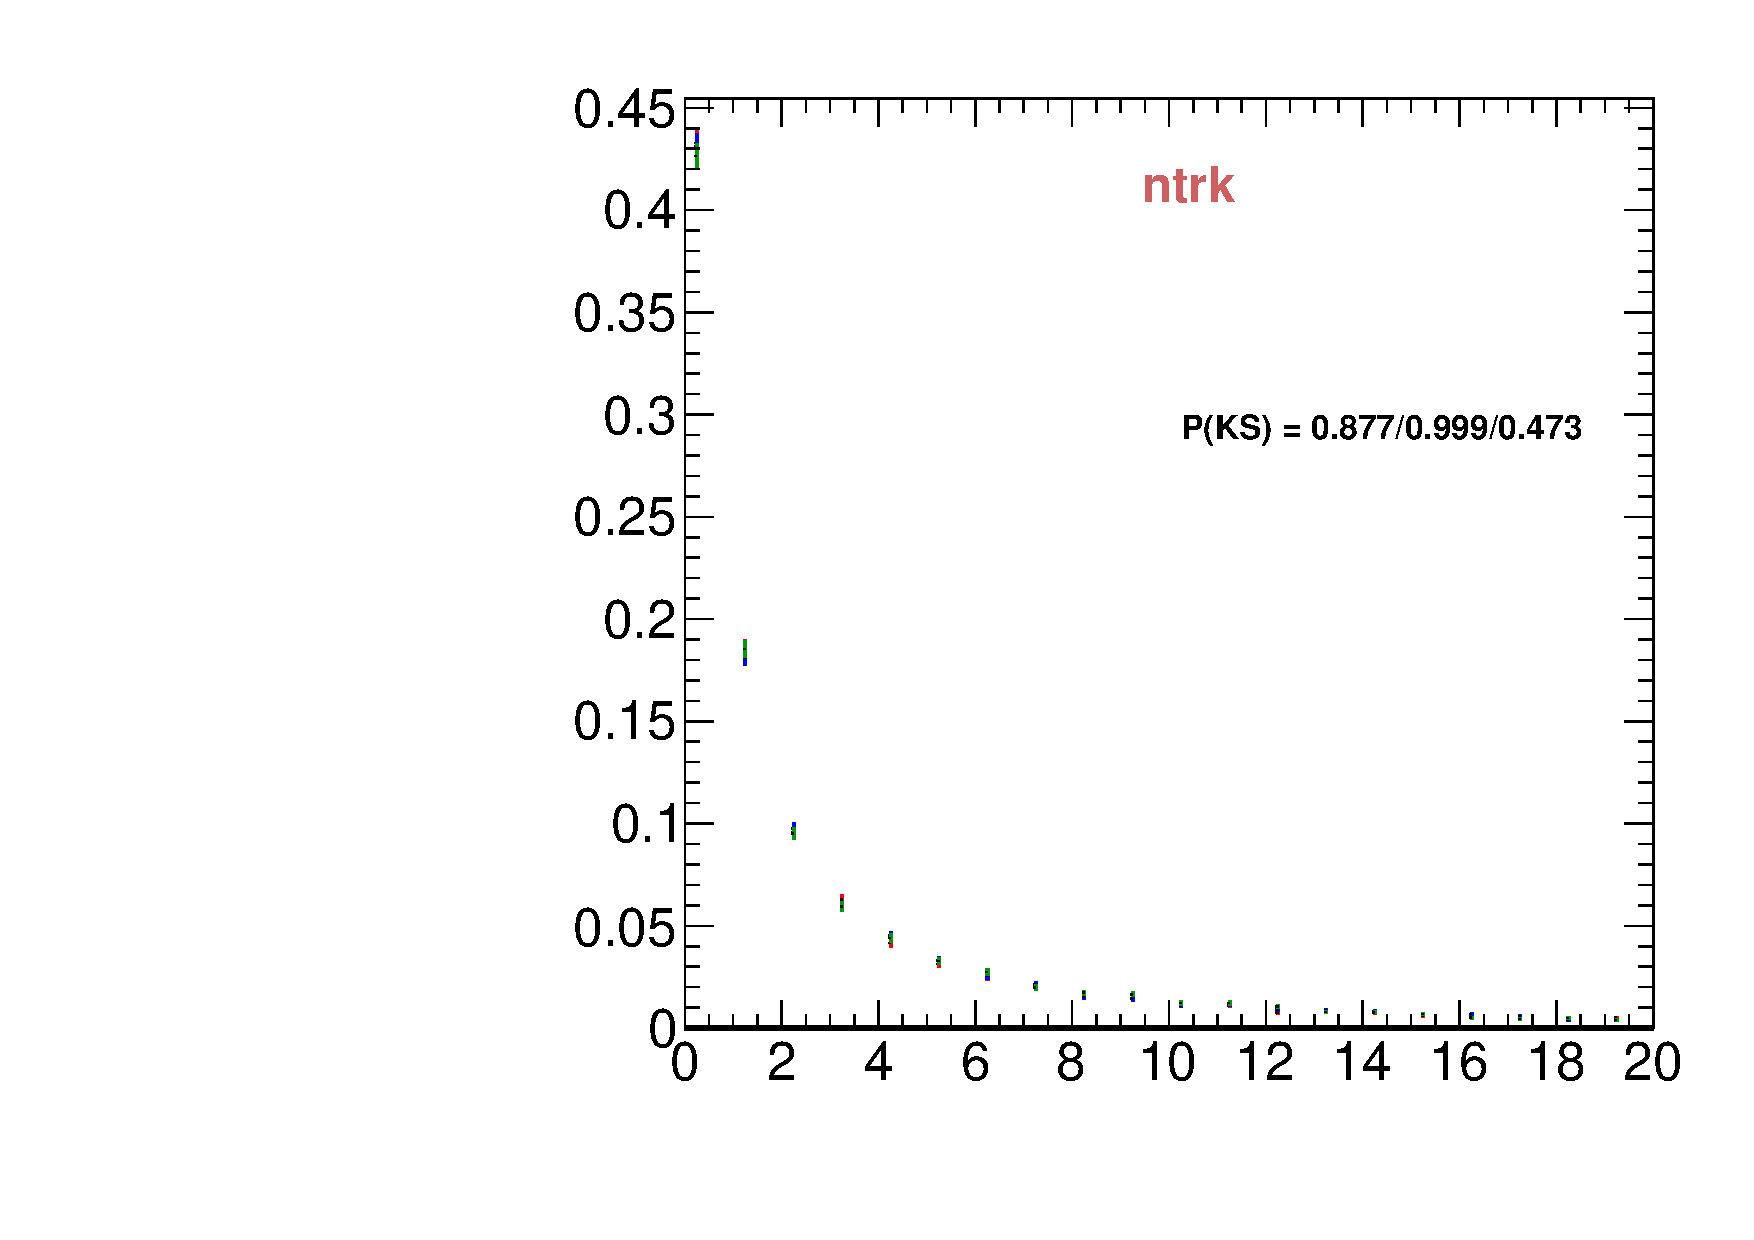
\includegraphics[width=\textwidth]{Figures/VariablesComparison/MC_barrel_figs_3h/ntrk}
                \label{fig:MC_barrel_ntrk_3h}
        \end{subfigure}
        \begin{subfigure}[b]{0.2\textwidth}
                \centering
                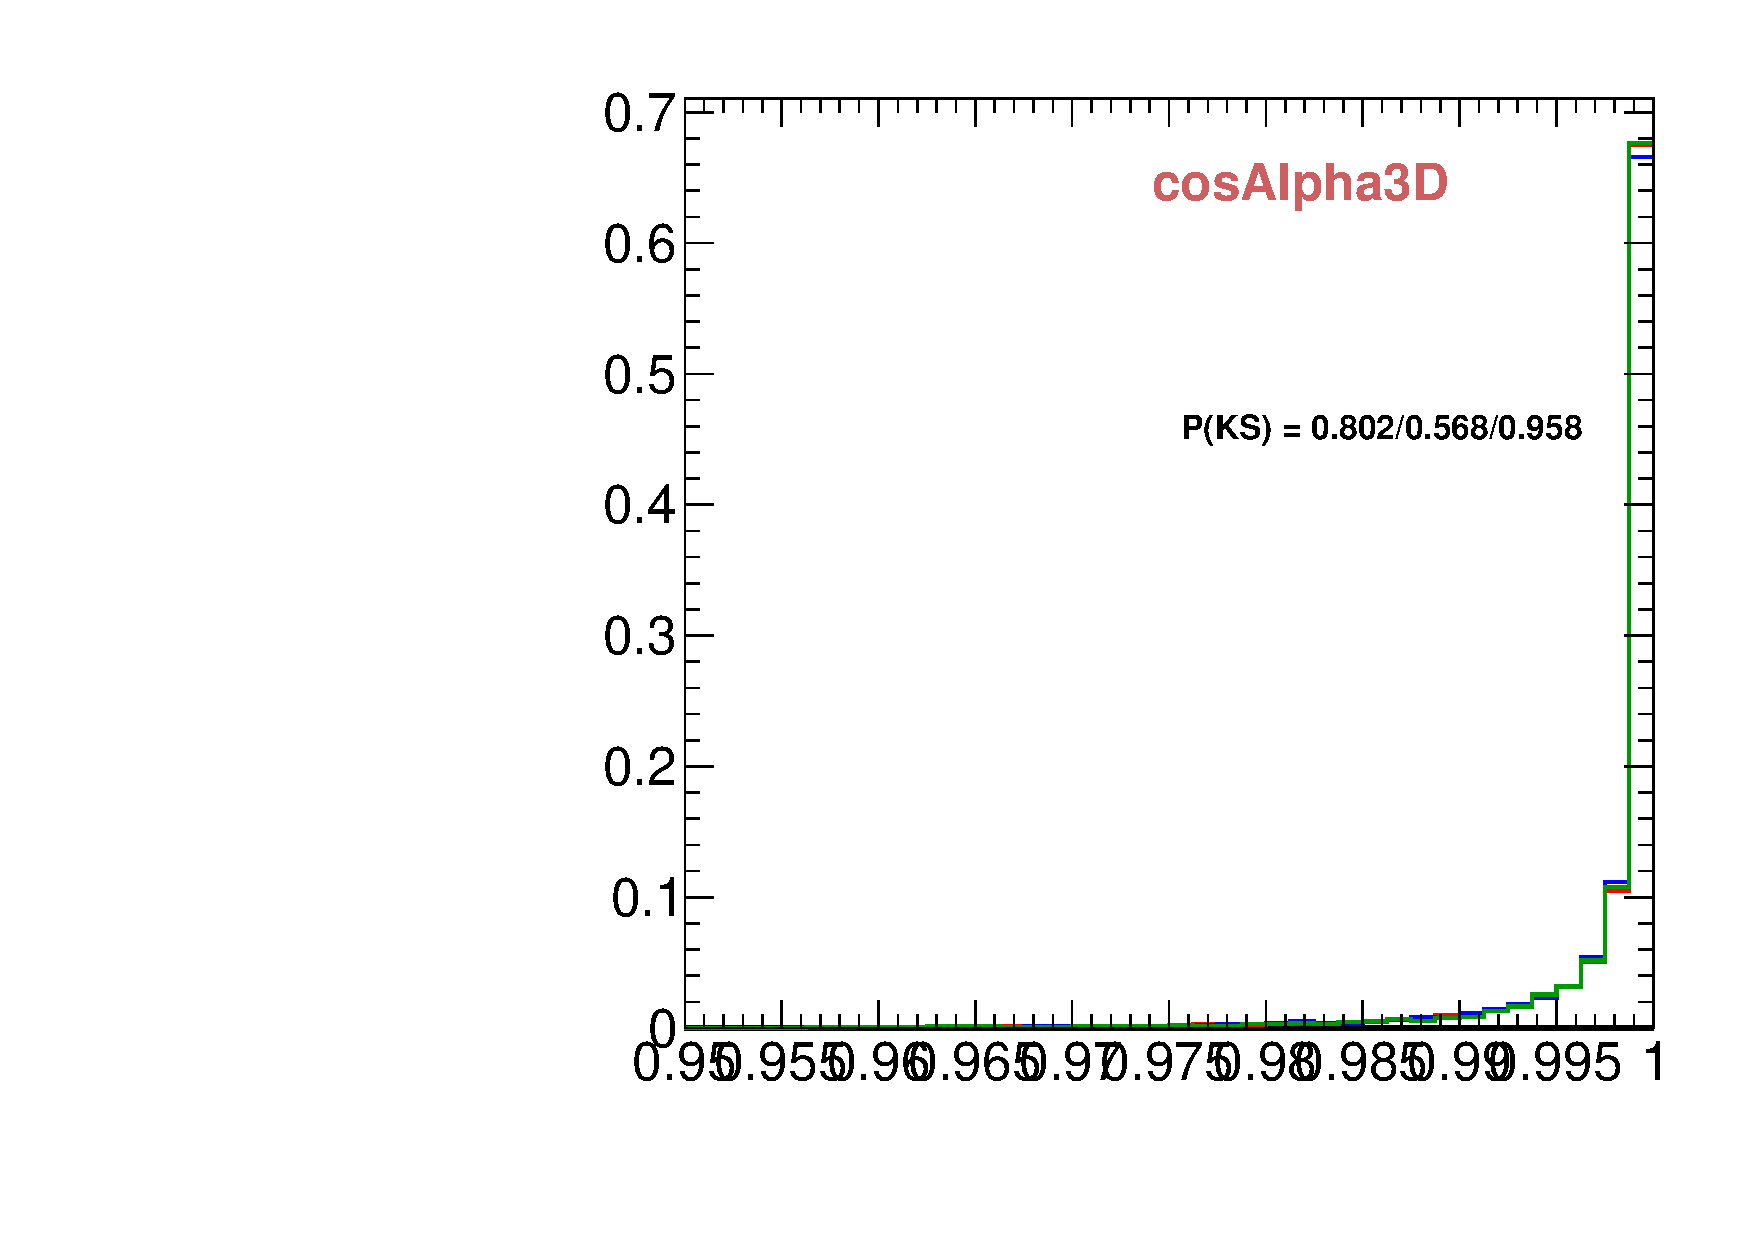
\includegraphics[width=\textwidth]{Figures/VariablesComparison/MC_barrel_figs_3h/cosAlpha3D}
                \label{fig:MC_barrel_cosAlpha3D_3h}
        \end{subfigure}
        \begin{subfigure}[b]{0.2\textwidth}
                \centering
                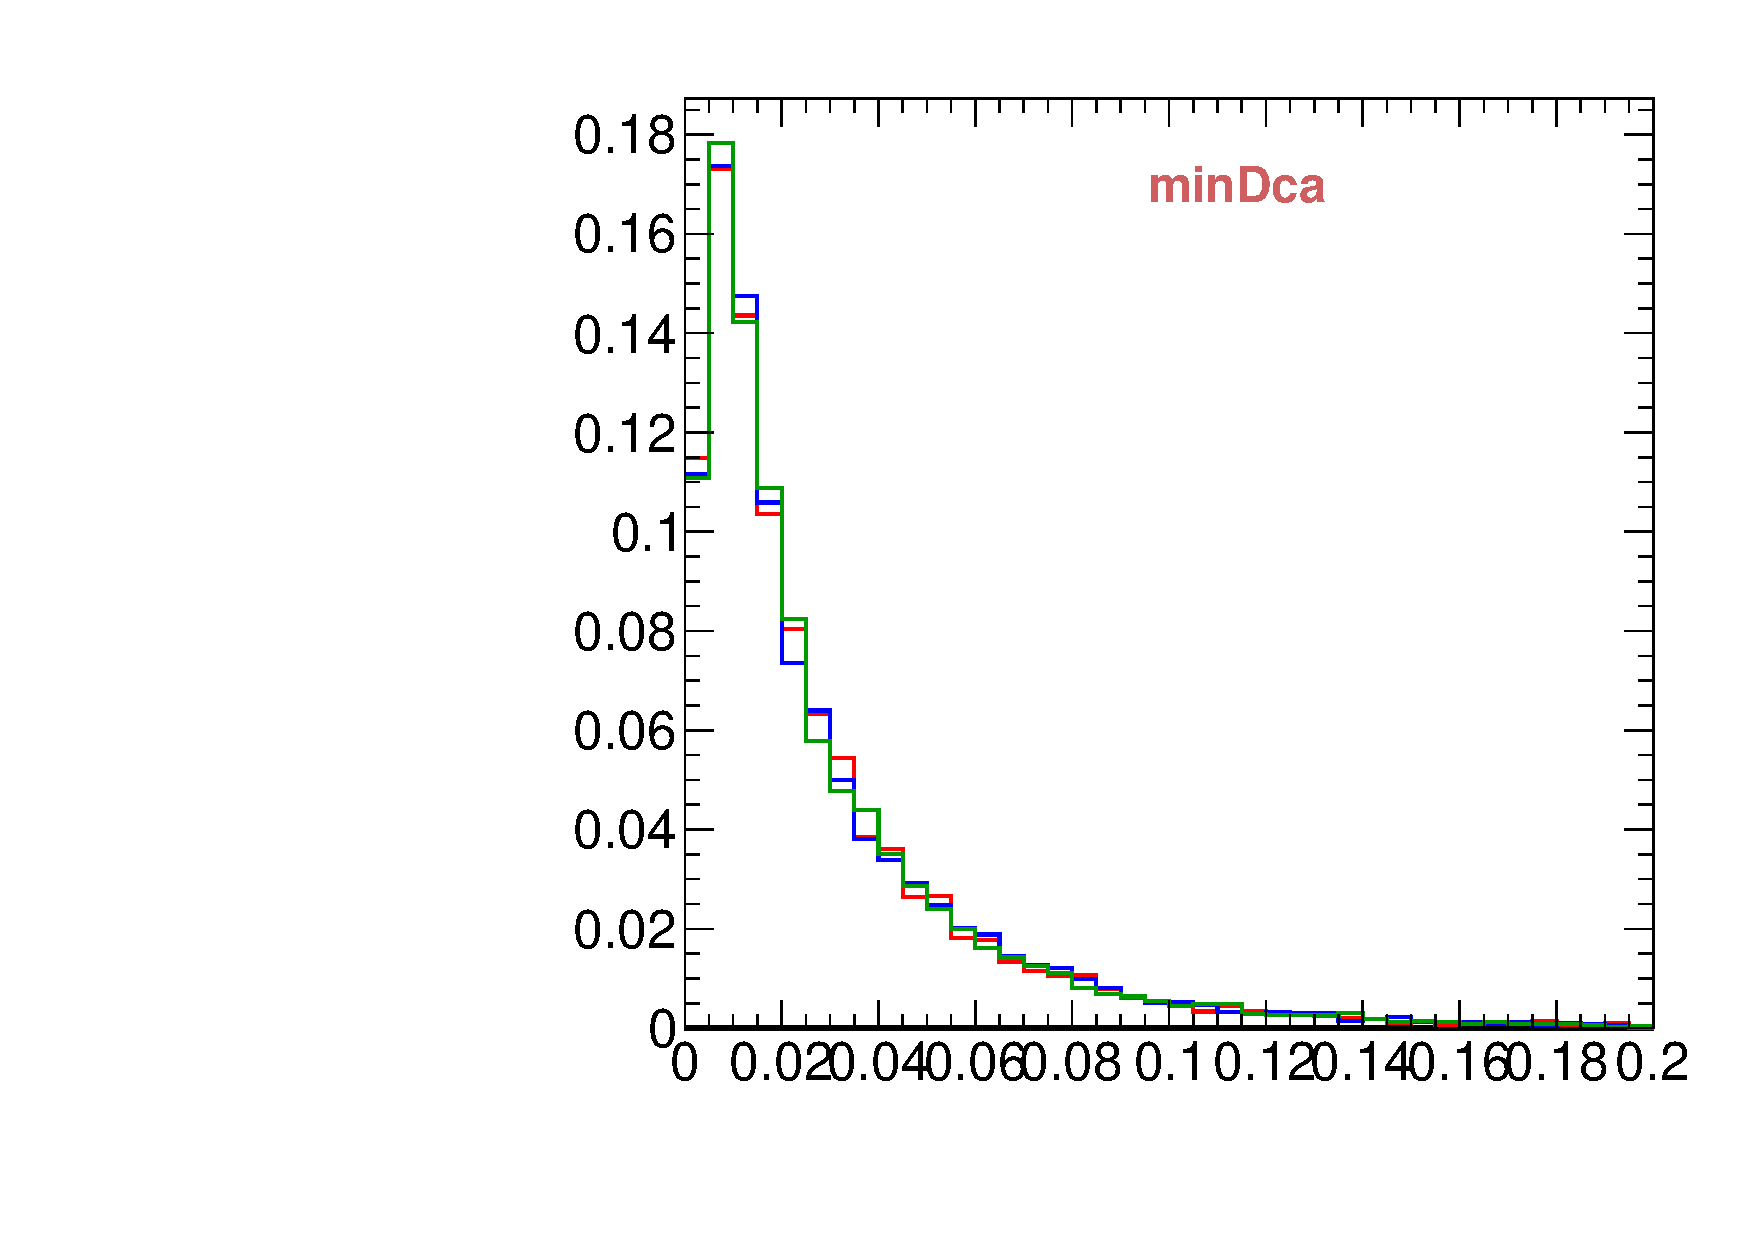
\includegraphics[width=\textwidth]{Figures/VariablesComparison/MC_barrel_figs_3h/minDca}
                \label{fig:MC_barrel_minDca_3h}
        \end{subfigure}
        \begin{subfigure}[b]{0.2\textwidth}
                \centering
                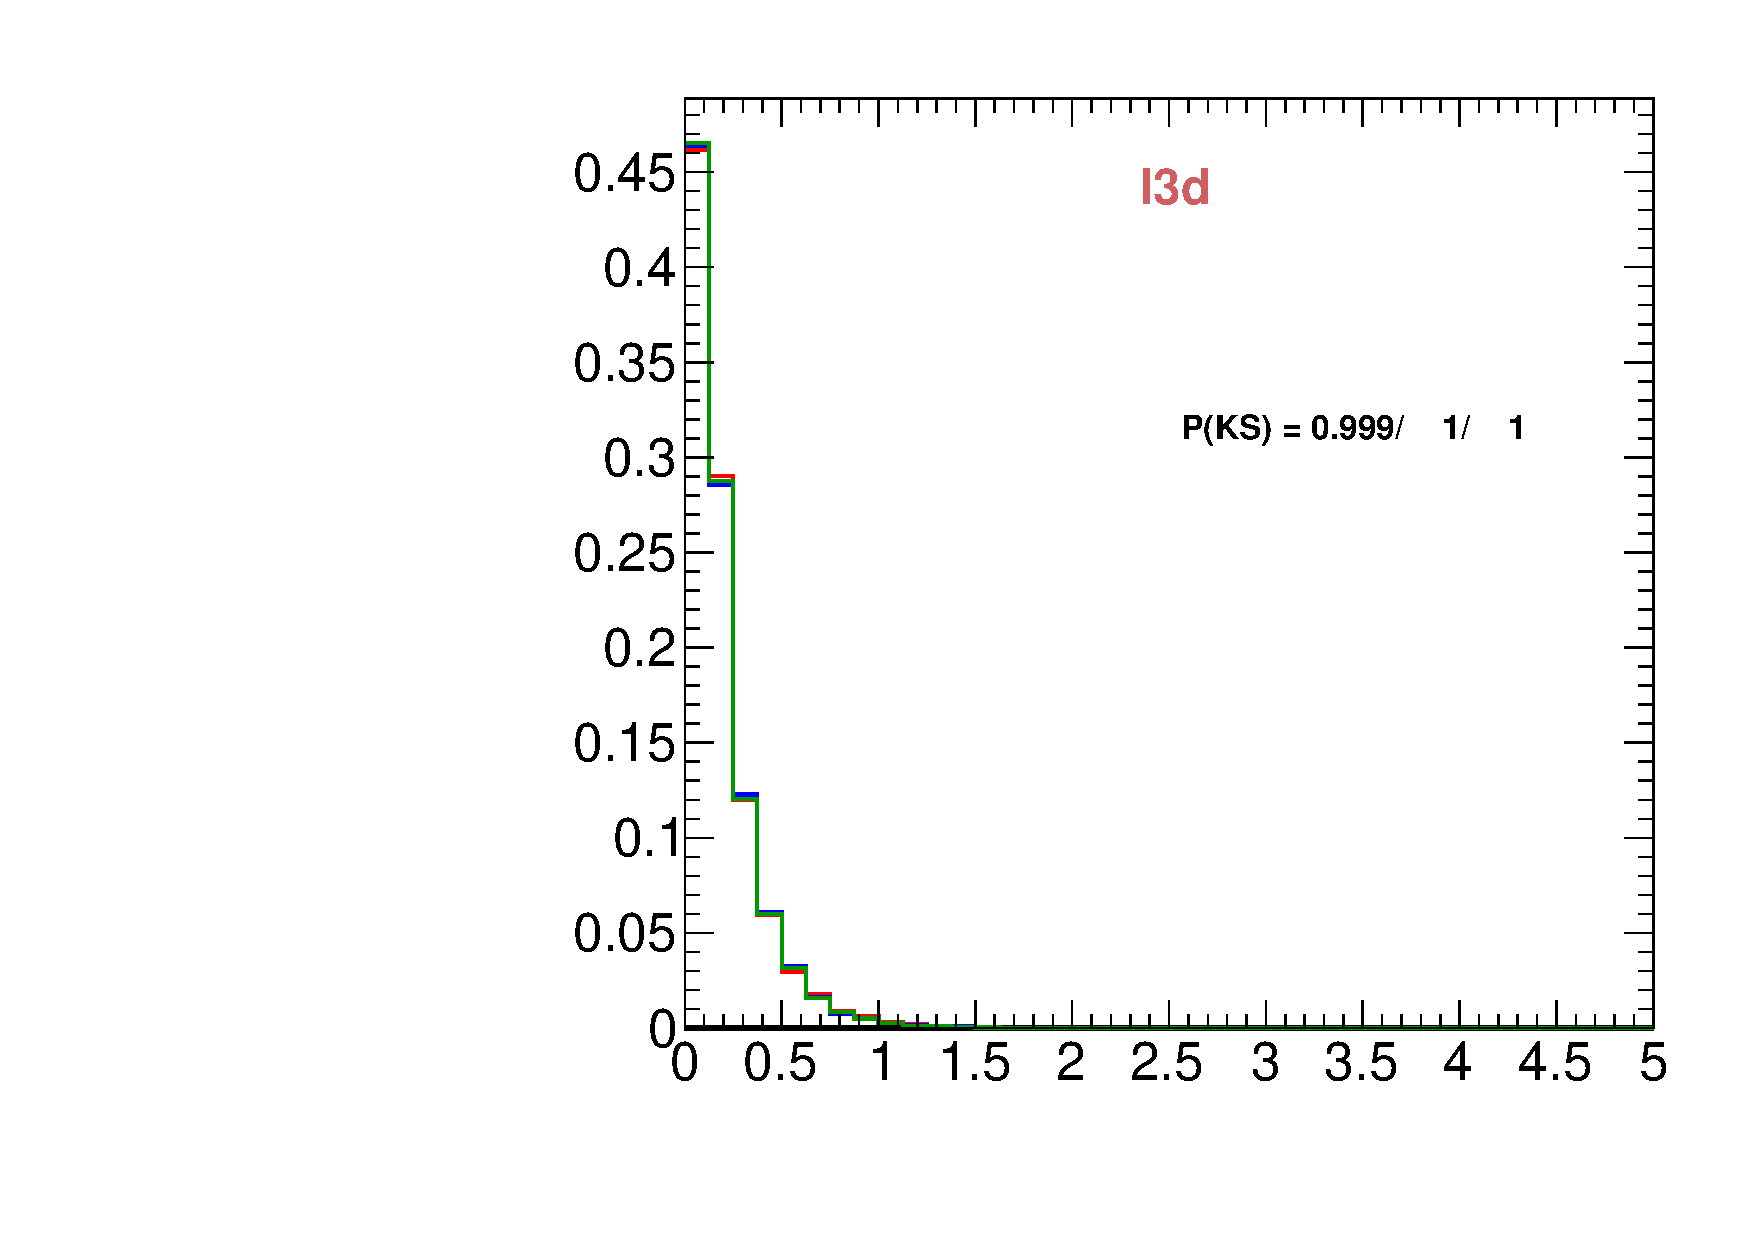
\includegraphics[width=\textwidth]{Figures/VariablesComparison/MC_barrel_figs_3h/l3d}
                \label{fig:MC_barrel_l3d_3h}
        \end{subfigure}
        \begin{subfigure}[b]{0.2\textwidth}
                \centering
                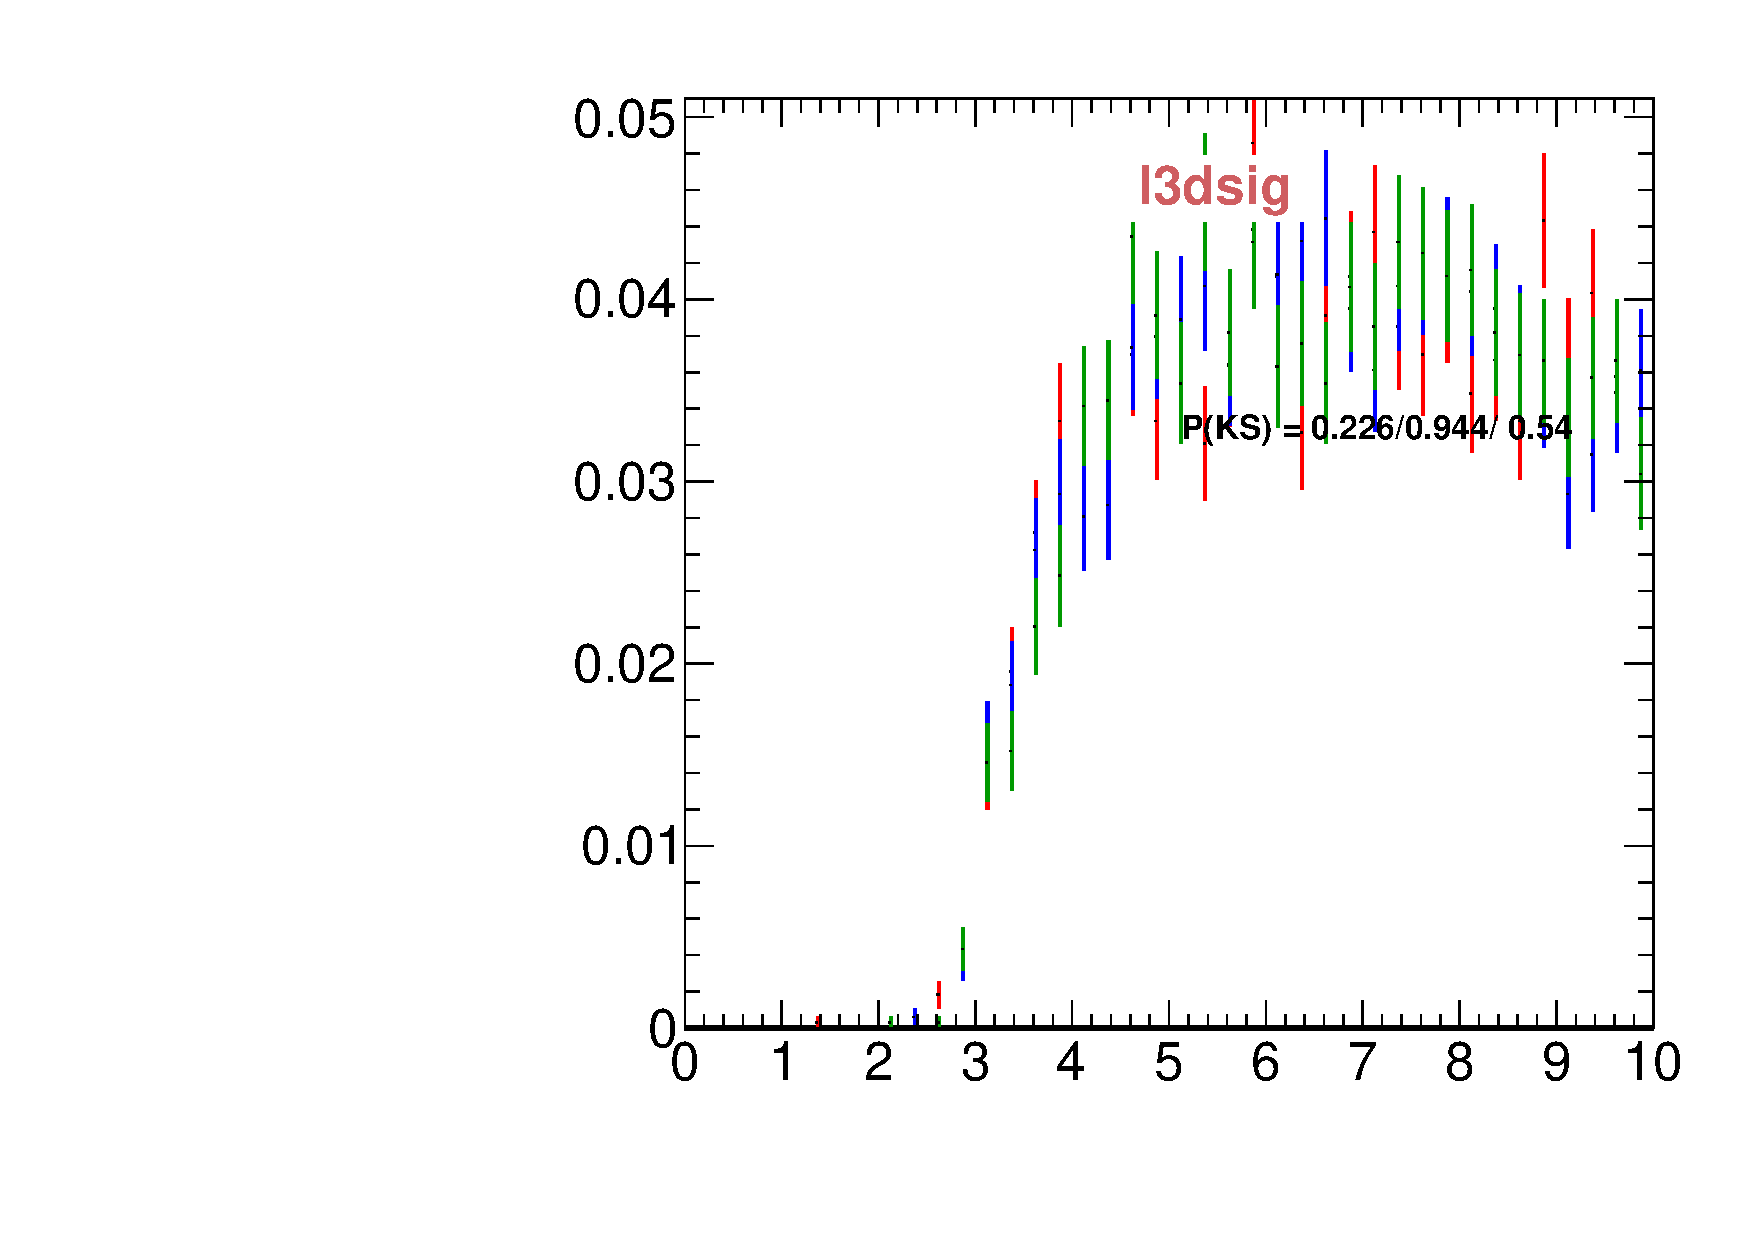
\includegraphics[width=\textwidth]{Figures/VariablesComparison/MC_barrel_figs_3h/l3dsig}
                \label{fig:MC_barrel_l3dsig_3h}
        \end{subfigure}
        \begin{subfigure}[b]{0.2\textwidth}
                \centering
                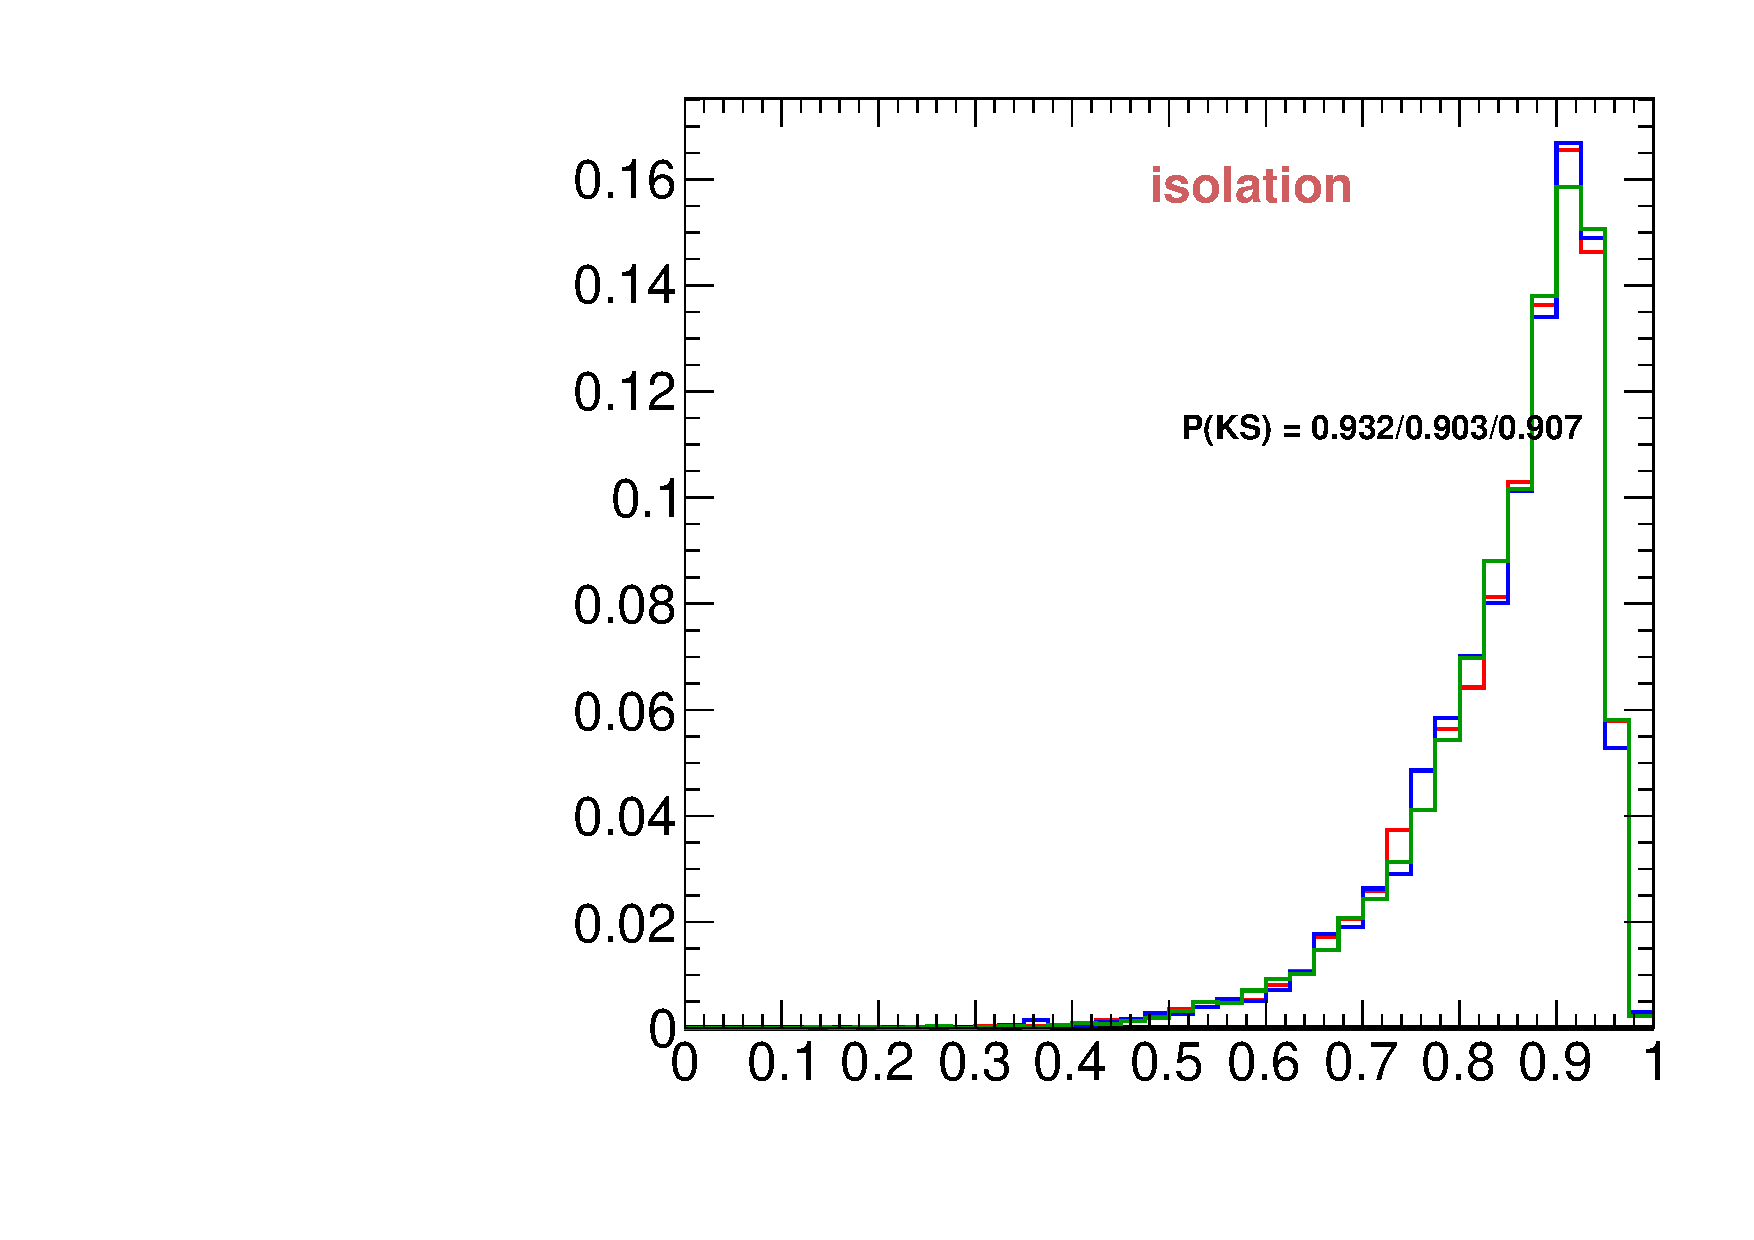
\includegraphics[width=\textwidth]{Figures/VariablesComparison/MC_barrel_figs_3h/isolation}
                \label{fig:MC_barrel_isolation_3h}
        \end{subfigure}
        \begin{subfigure}[b]{0.2\textwidth}
                \centering
                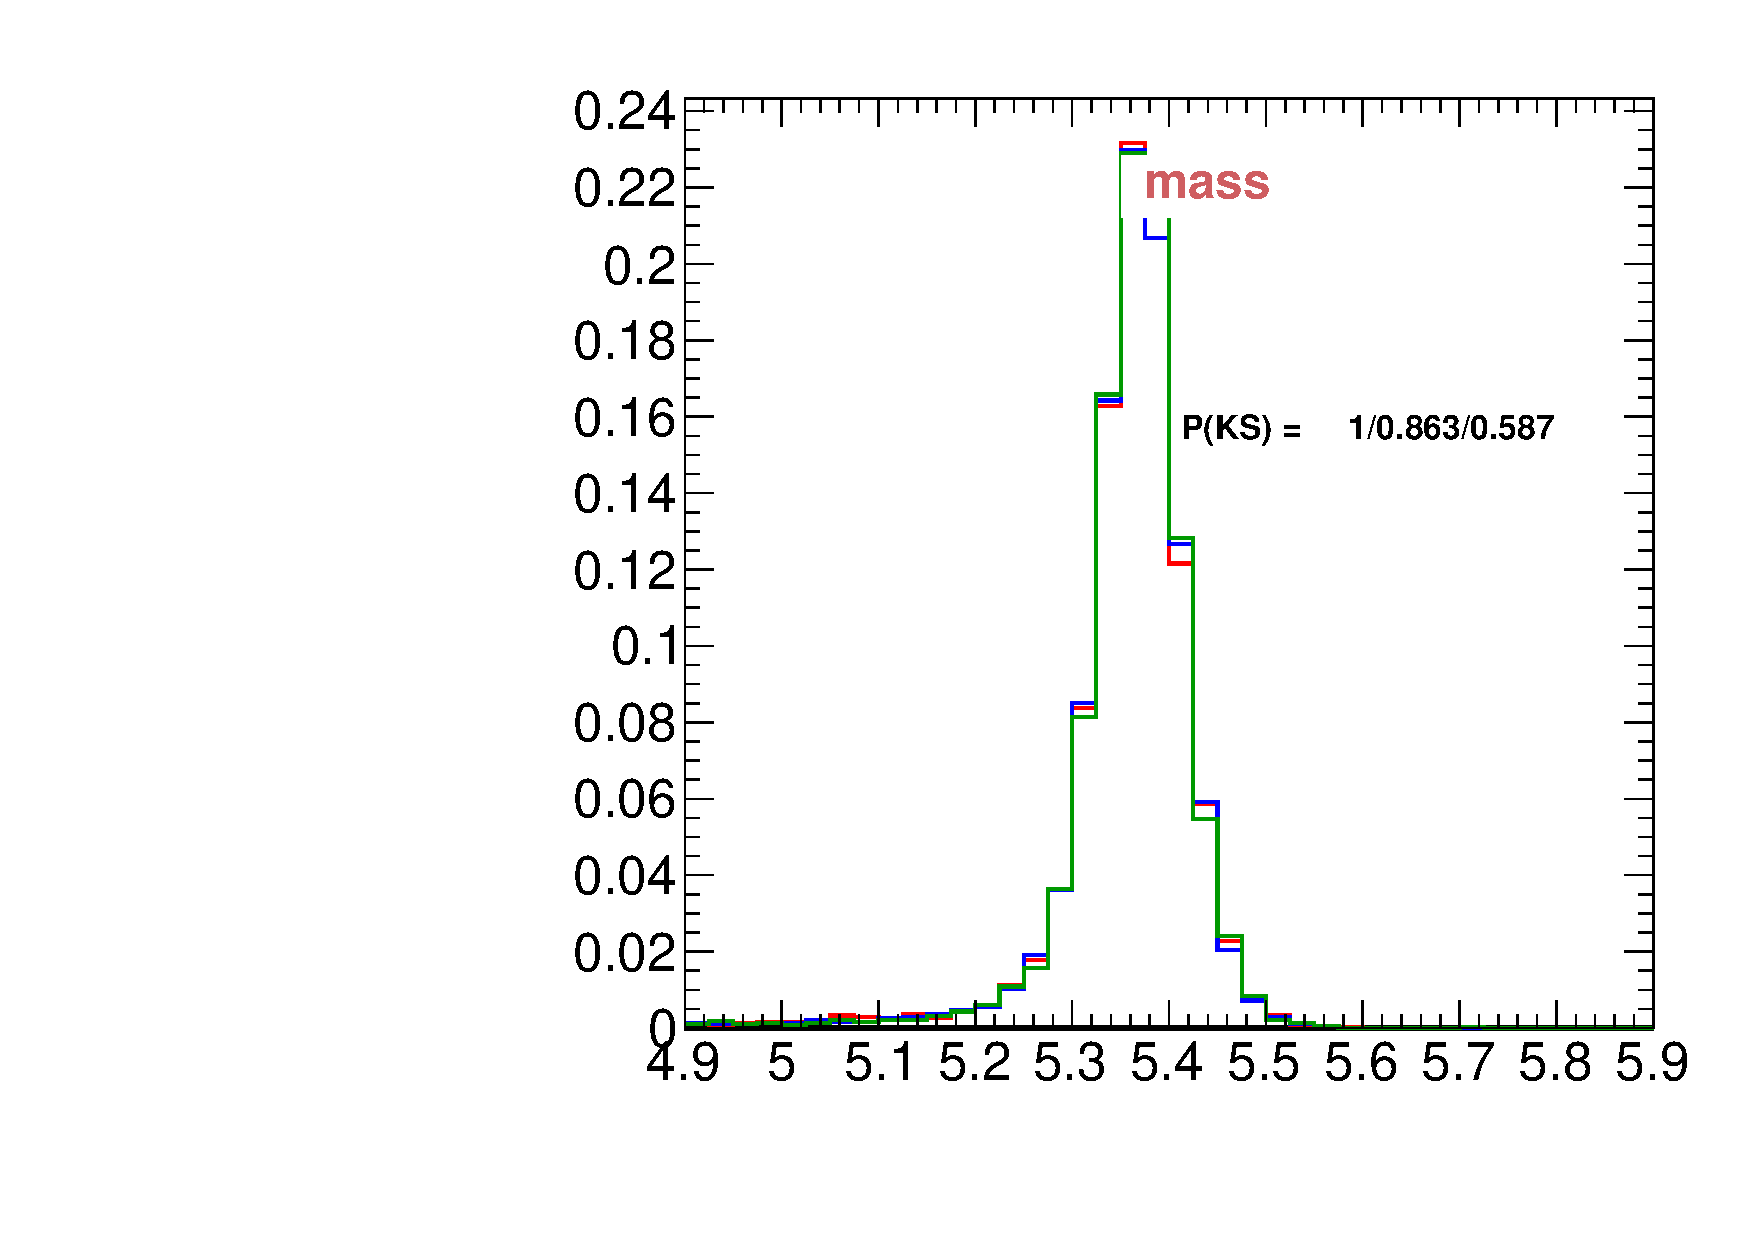
\includegraphics[width=\textwidth]{Figures/VariablesComparison/MC_barrel_figs_3h/mass}
                \label{fig:MC_barrel_mass_3h}
        \end{subfigure}
        \begin{subfigure}[b]{0.2\textwidth}
                \centering
                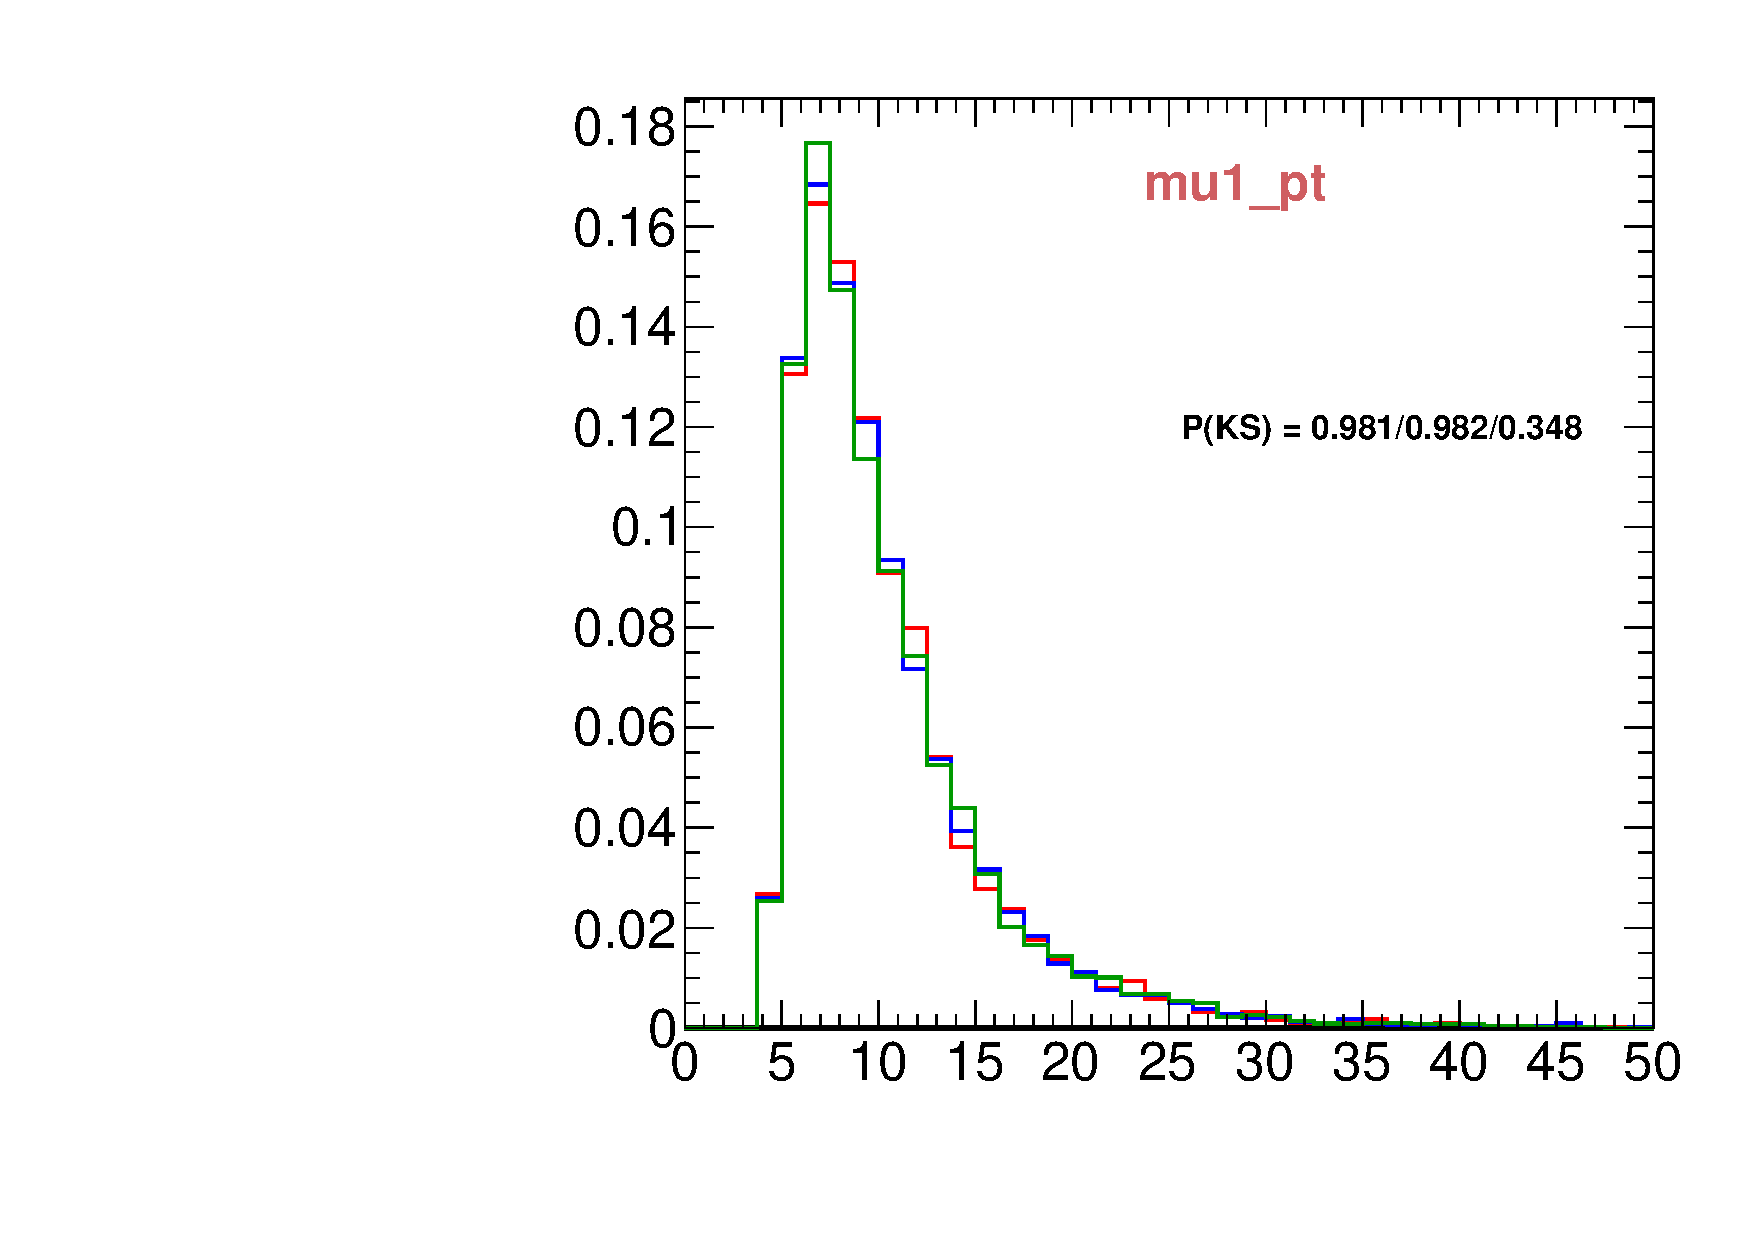
\includegraphics[width=\textwidth]{Figures/VariablesComparison/MC_barrel_figs_3h/mu1_pt}
                \label{fig:MC_barrel_mu1_pt_3h}
        \end{subfigure}
        \begin{subfigure}[b]{0.2\textwidth}
                \centering
                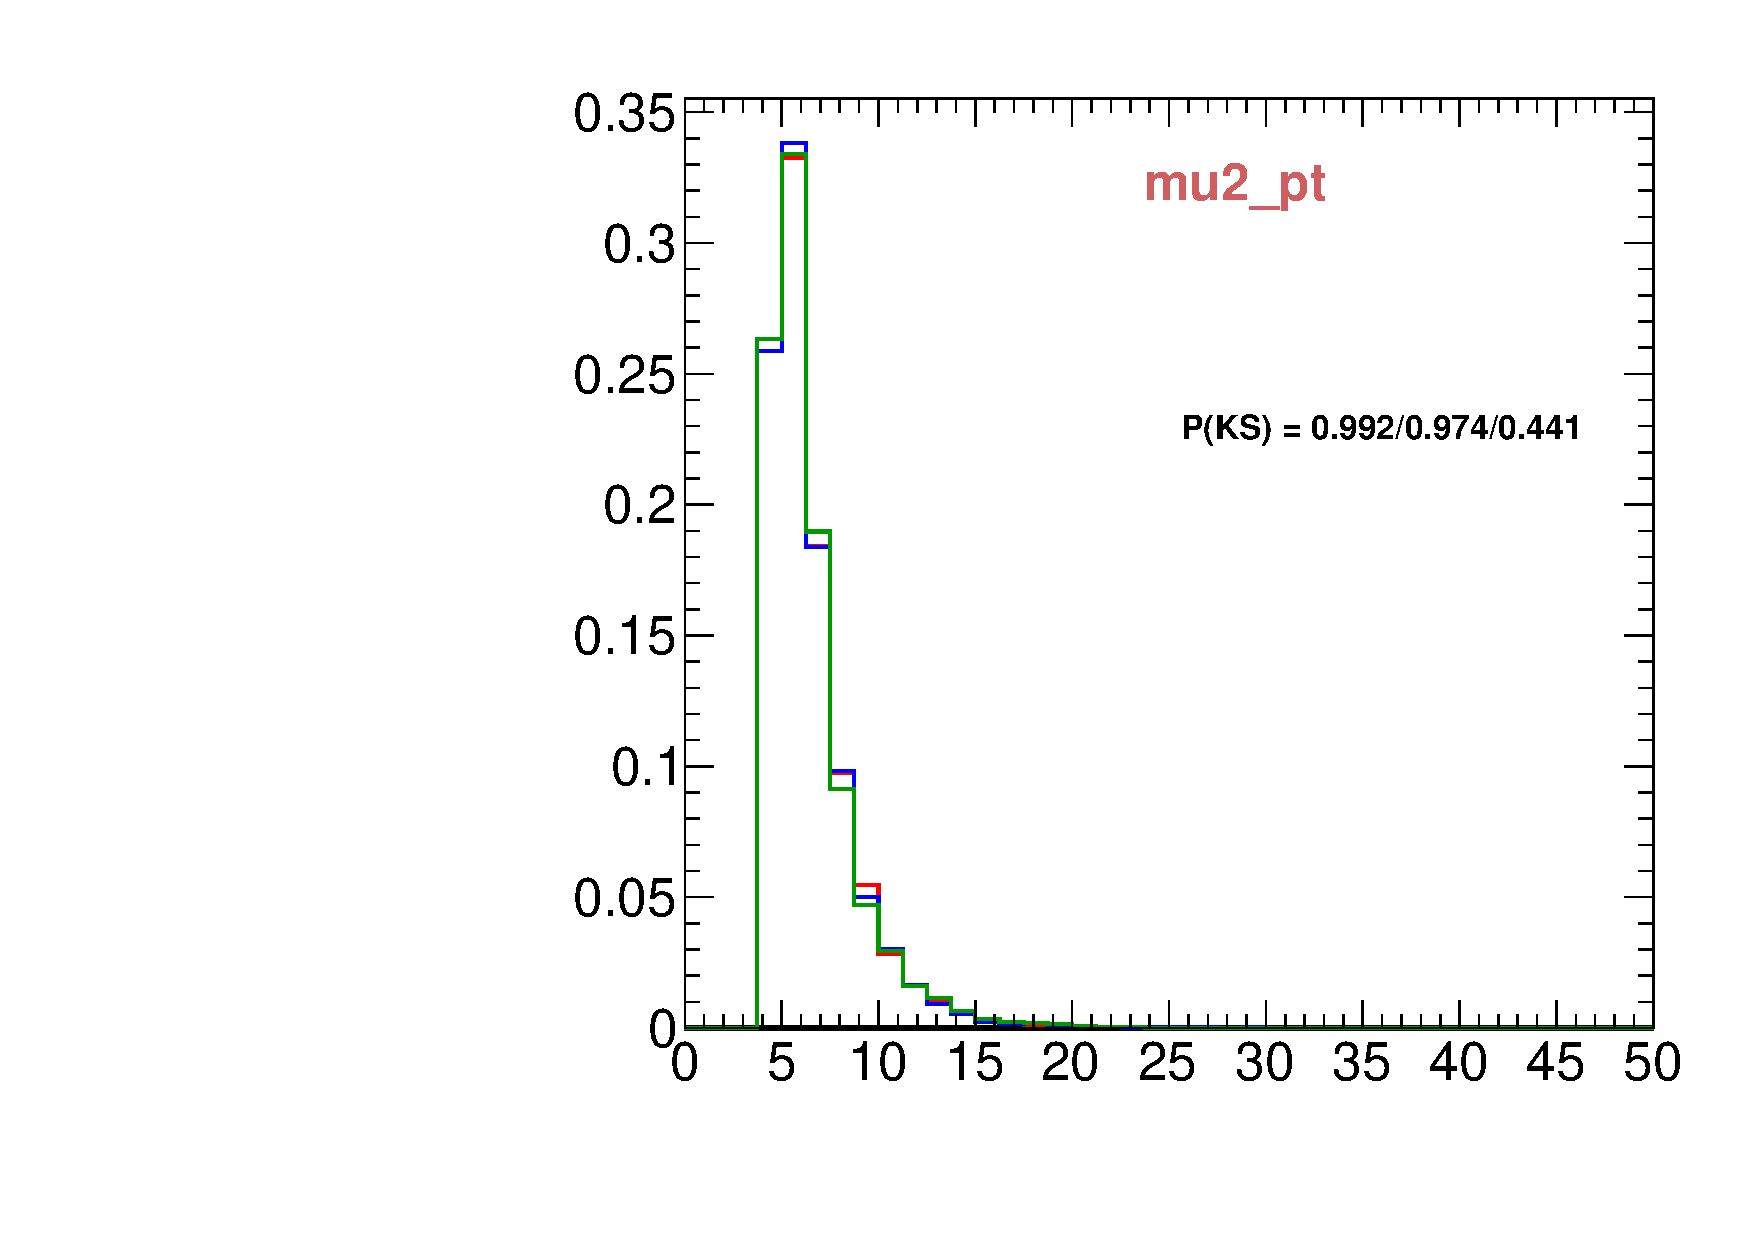
\includegraphics[width=\textwidth]{Figures/VariablesComparison/MC_barrel_figs_3h/mu2_pt}
                \label{fig:MC_barrel_mu2_pt_3h}
        \end{subfigure}
        \begin{subfigure}[b]{0.2\textwidth}
                \centering
                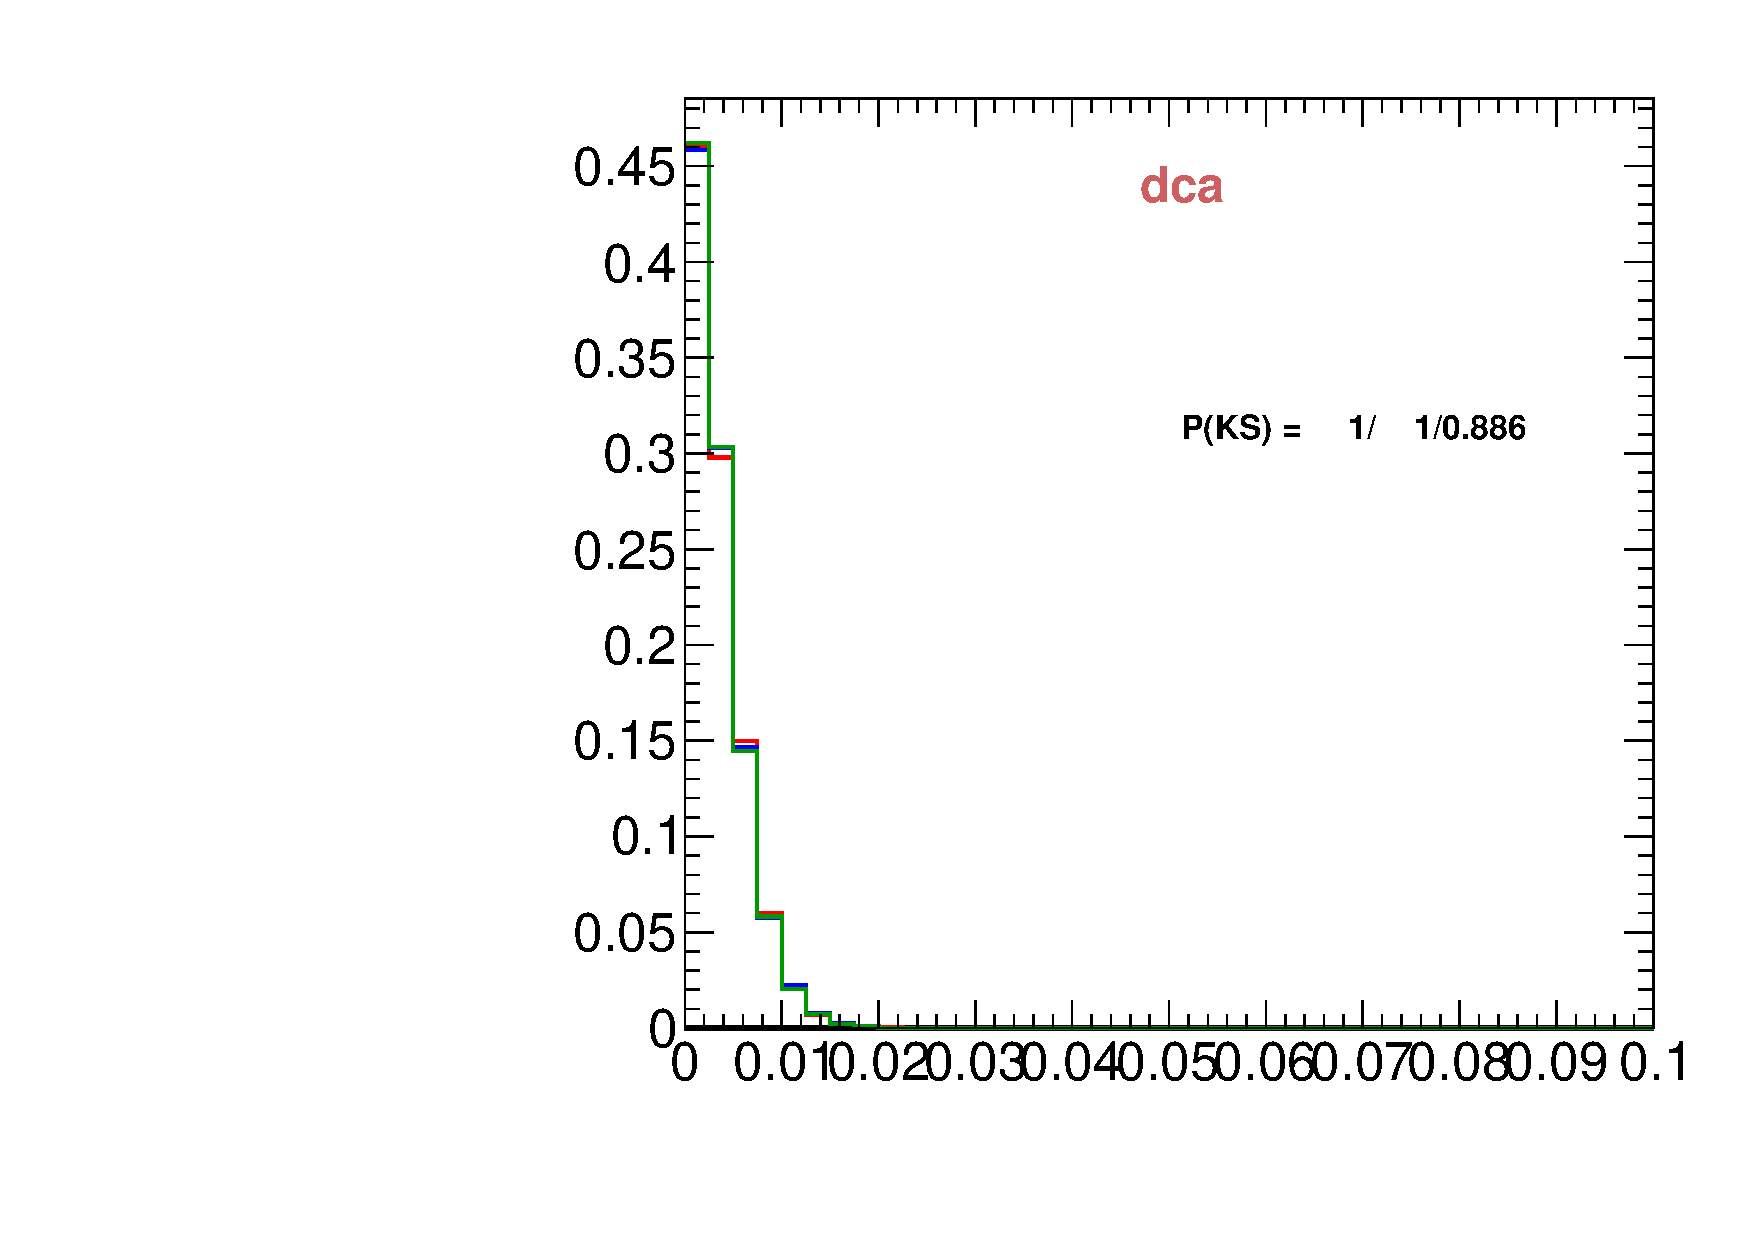
\includegraphics[width=\textwidth]{Figures/VariablesComparison/MC_barrel_figs_3h/dca}
                \label{fig:MC_barrel_dca_3h}
        \end{subfigure}
        \begin{subfigure}[b]{0.2\textwidth}
                \centering
                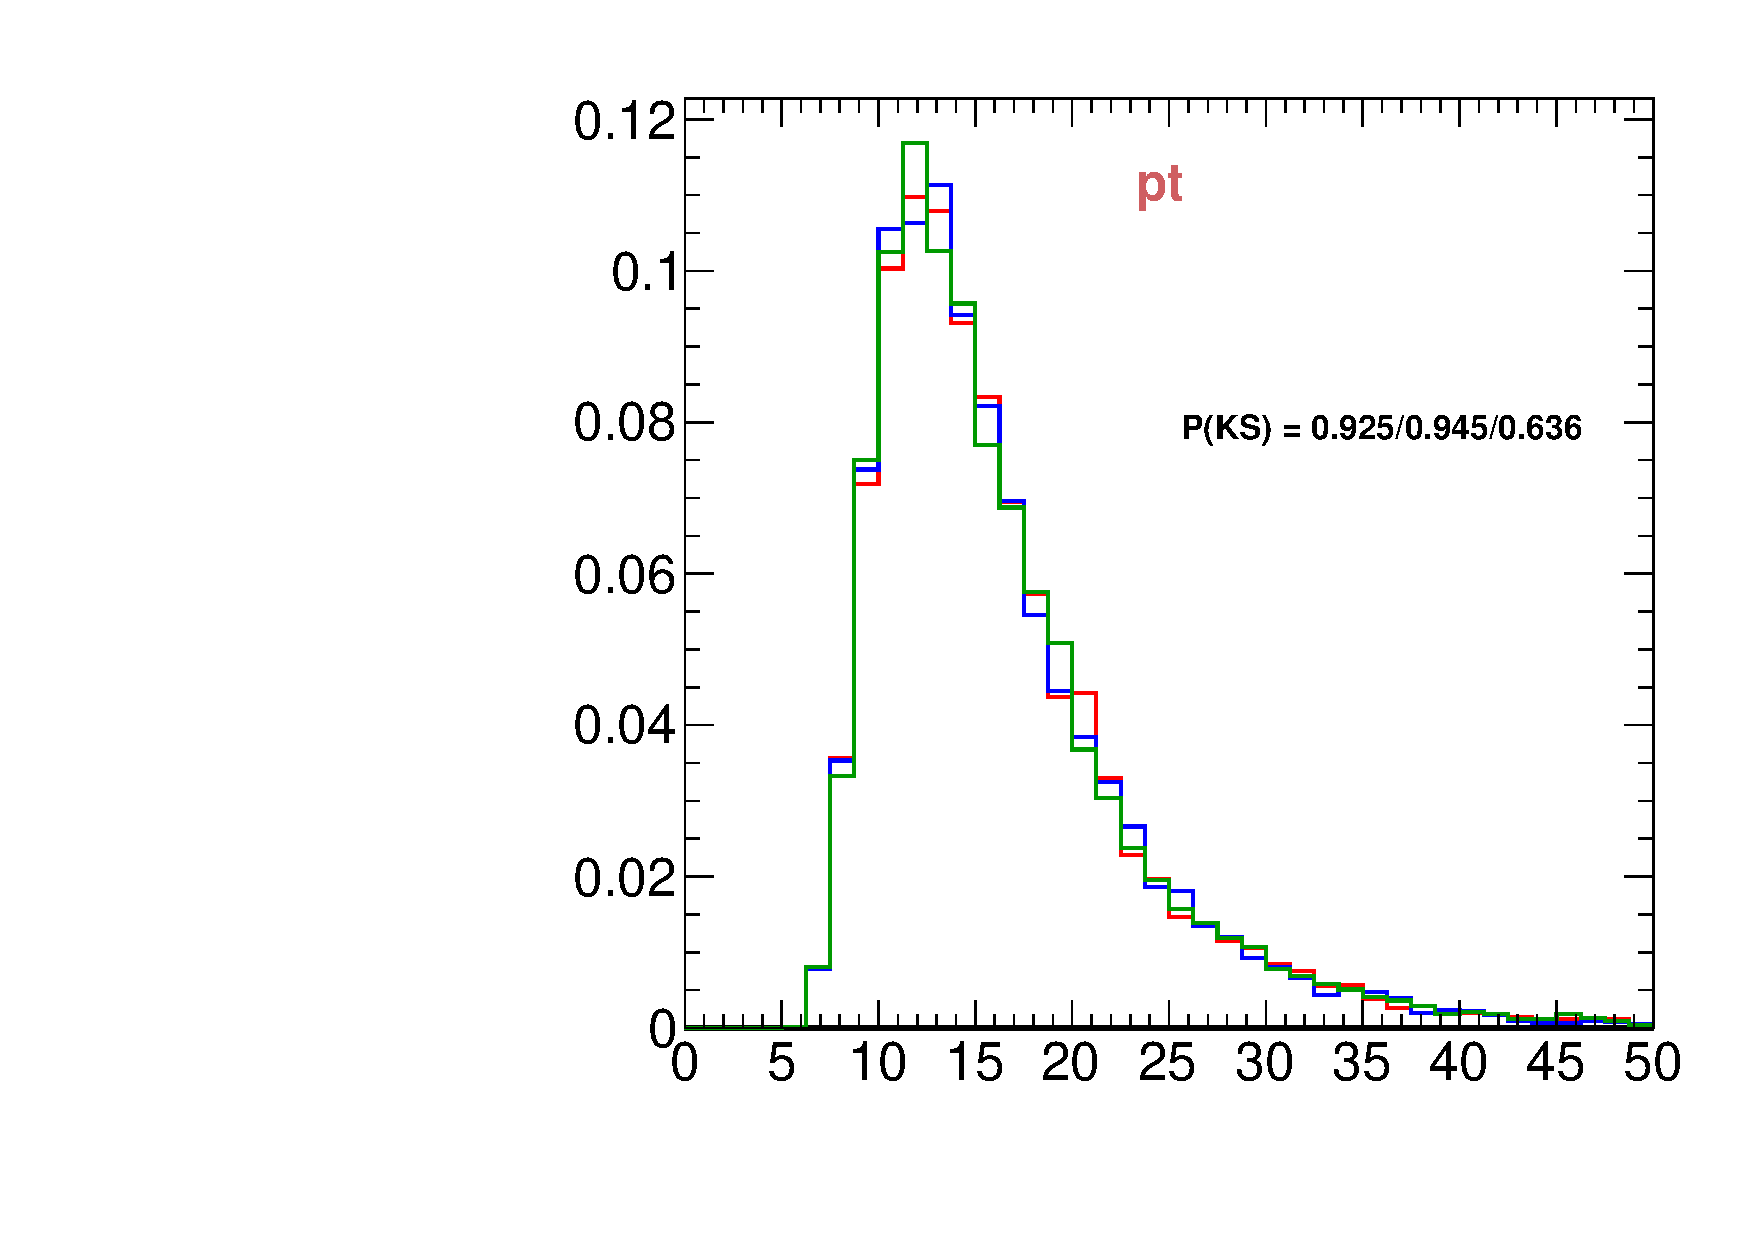
\includegraphics[width=\textwidth]{Figures/VariablesComparison/MC_barrel_figs_3h/pt}
                \label{fig:MC_barrel_pt_3h}
        \end{subfigure}
        \begin{subfigure}[b]{0.2\textwidth}
                \centering
                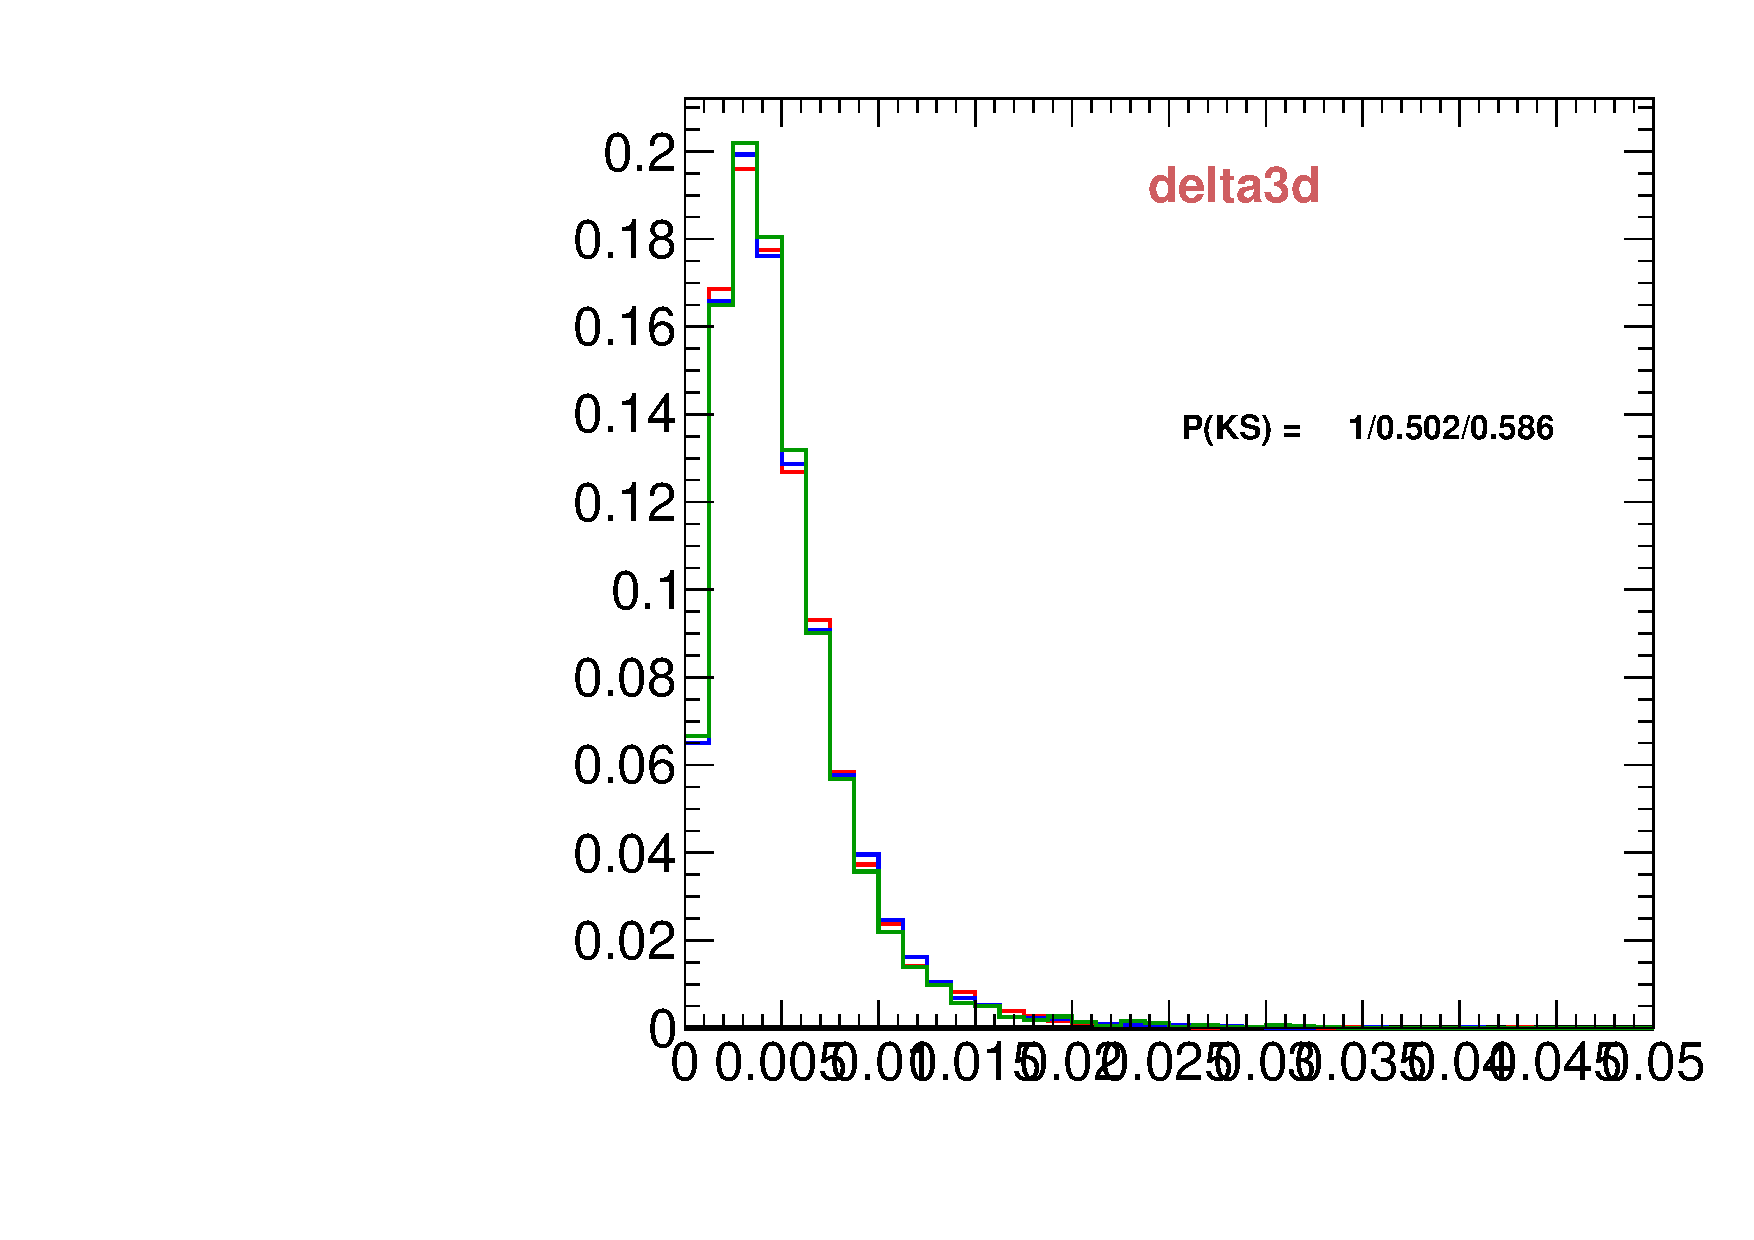
\includegraphics[width=\textwidth]{Figures/VariablesComparison/MC_barrel_figs_3h/delta3d}
                \label{fig:MC_barrel_delta3d_3h}
        \end{subfigure}
        \begin{subfigure}[b]{0.2\textwidth}
                \centering
                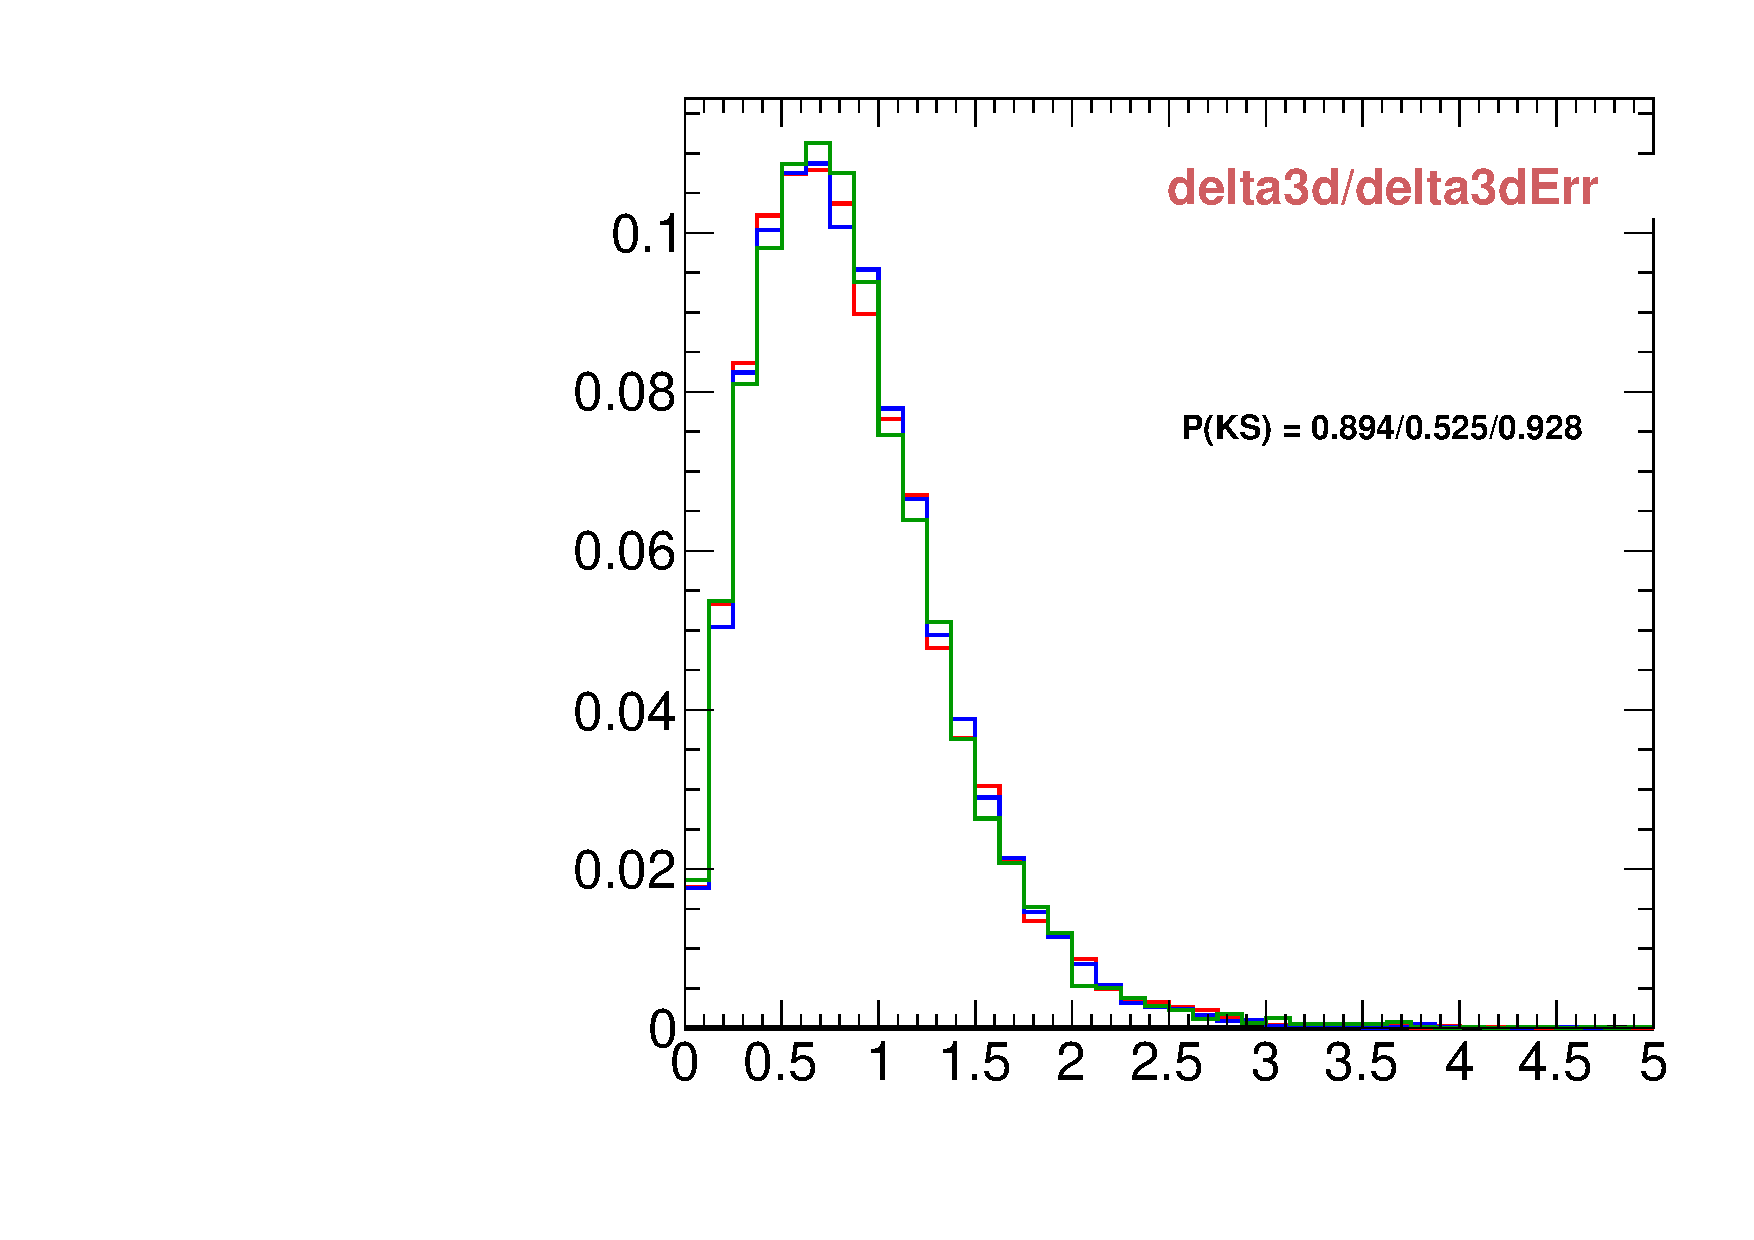
\includegraphics[width=\textwidth]{Figures/VariablesComparison/MC_barrel_figs_3h/delta3dErr}
                \label{fig:MC_barrel_delta3d/delta3dErr_3h}
        \end{subfigure}
        \begin{subfigure}[b]{0.2\textwidth}
                \centering
                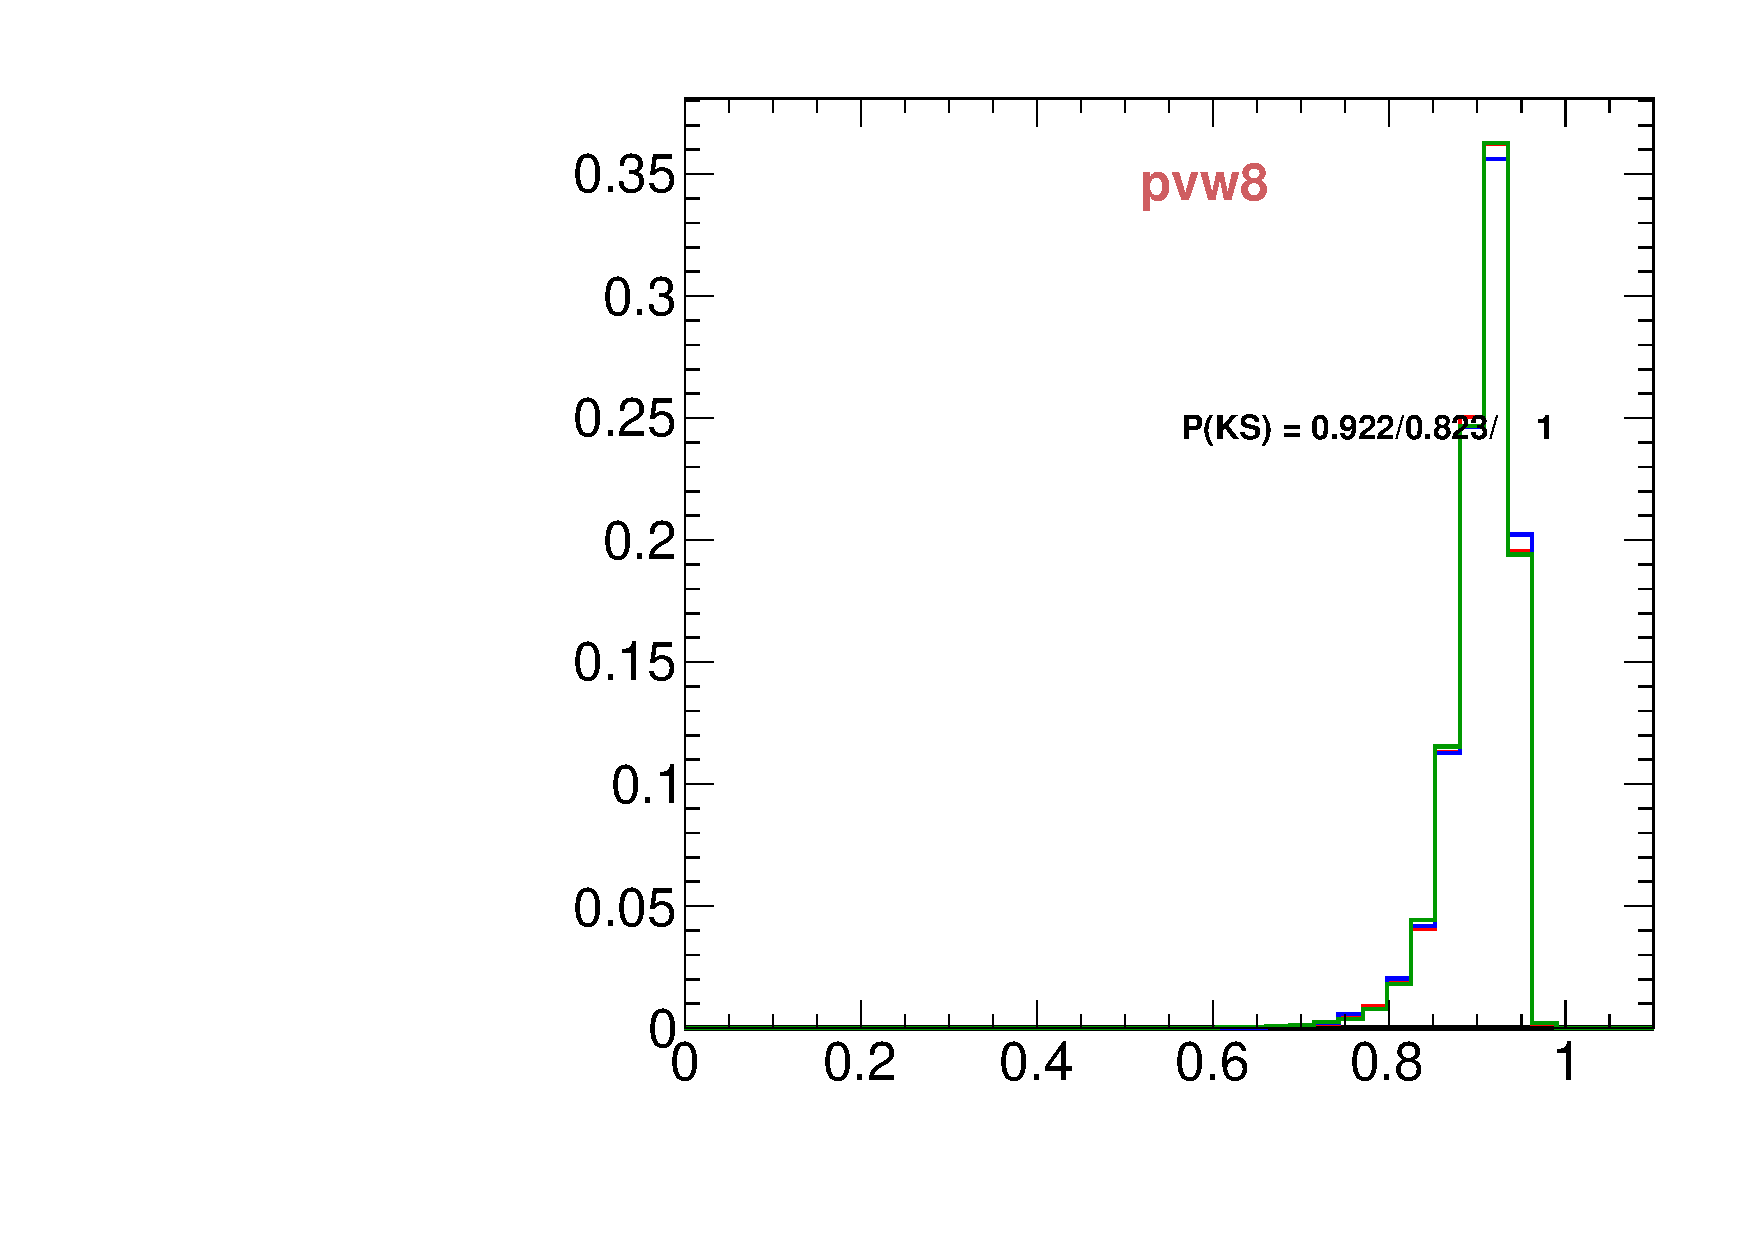
\includegraphics[width=\textwidth]{Figures/VariablesComparison/MC_barrel_figs_3h/pvw8}
                \label{fig:MC_barrel_pvw8_3h}
        \end{subfigure}
        \begin{subfigure}[b]{0.2\textwidth}
                \centering
                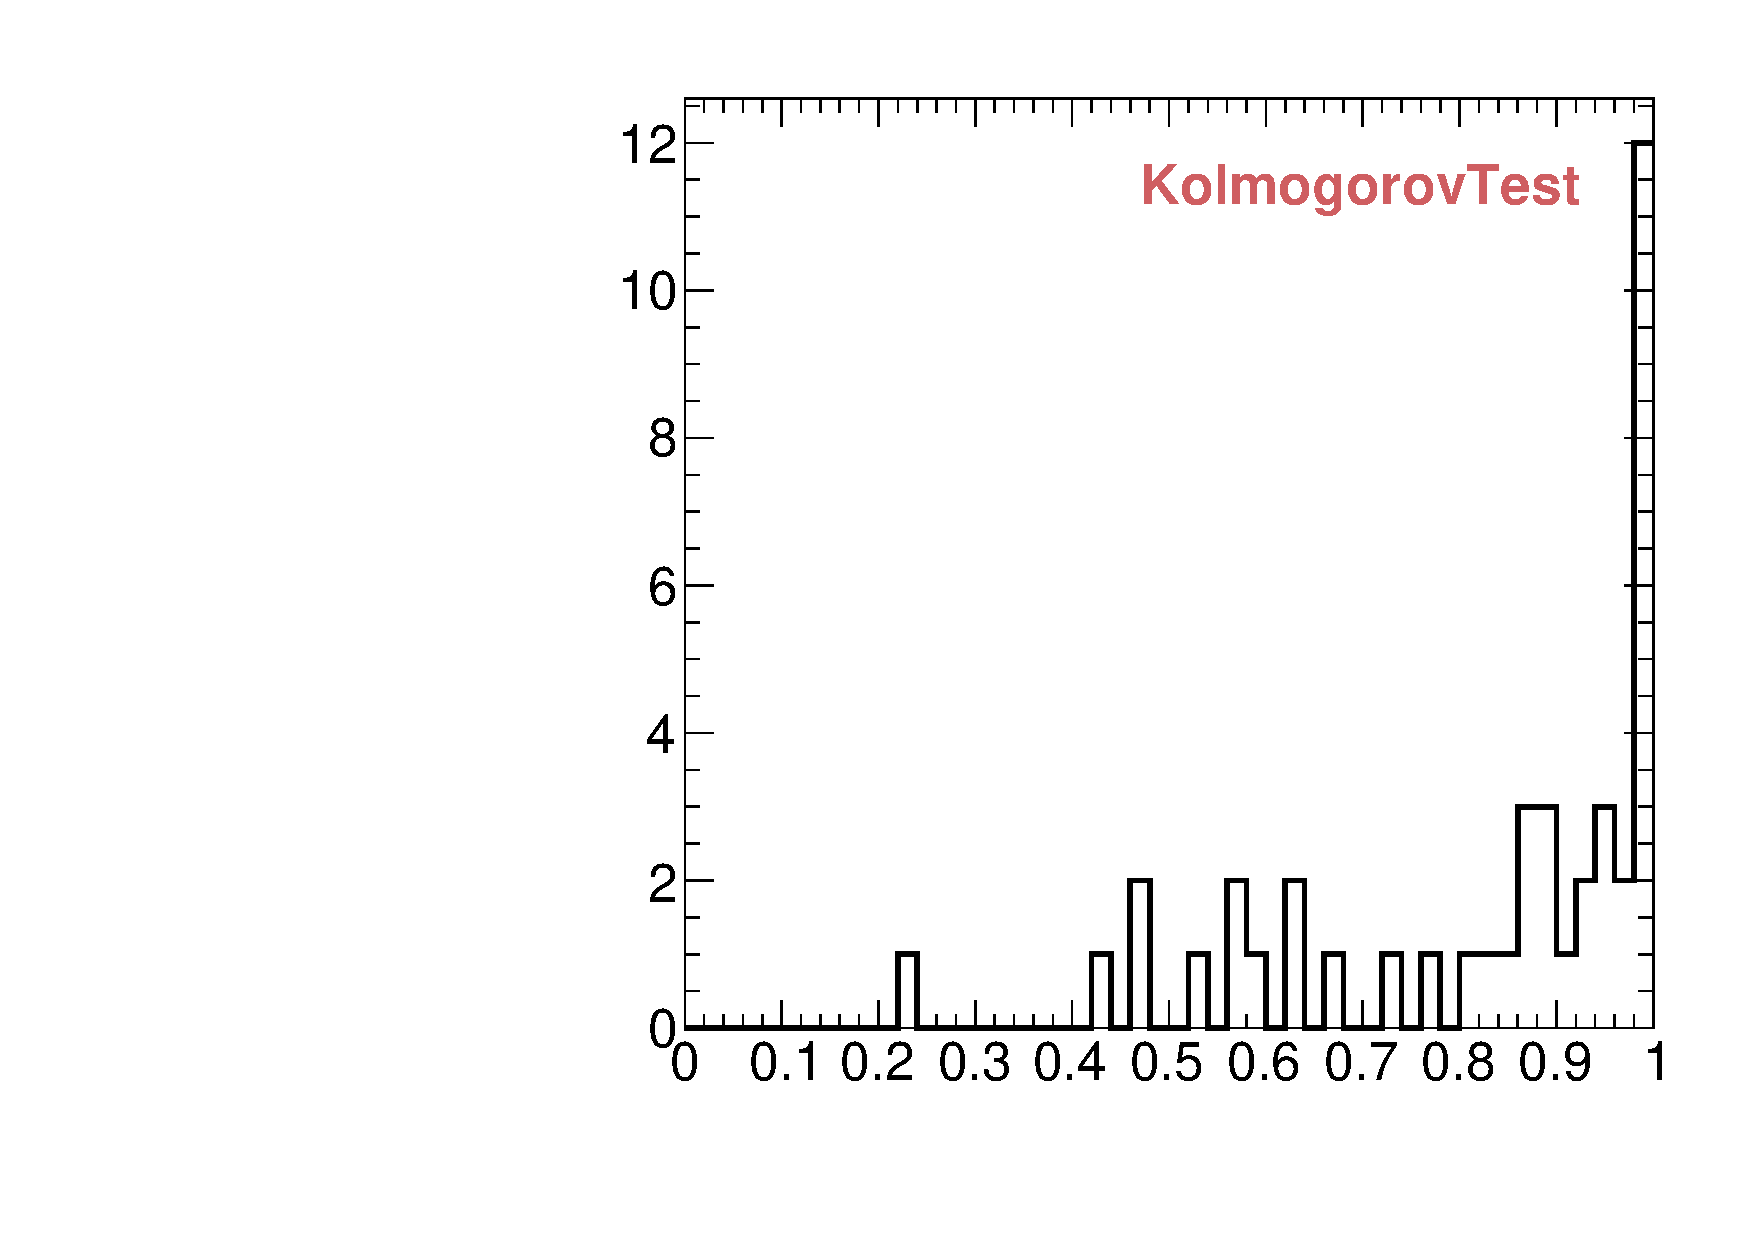
\includegraphics[width=\textwidth]{Figures/VariablesComparison/MC_barrel_figs_3h/KS}
                \label{fig:MC_barrel_KS_3h}
        \end{subfigure}
        \caption{Overlay of BDT training variable distributions in Signal MC for events of the three subsets in the barrel. The plot on the bottom right summarizes all KS probablities.}
        \label{fig:MC_barrel_figs_3h}
\end{sidewaysfigure}


\begin{sidewaysfigure}
        \centering
        \begin{subfigure}[b]{0.2\textwidth}
                \centering
                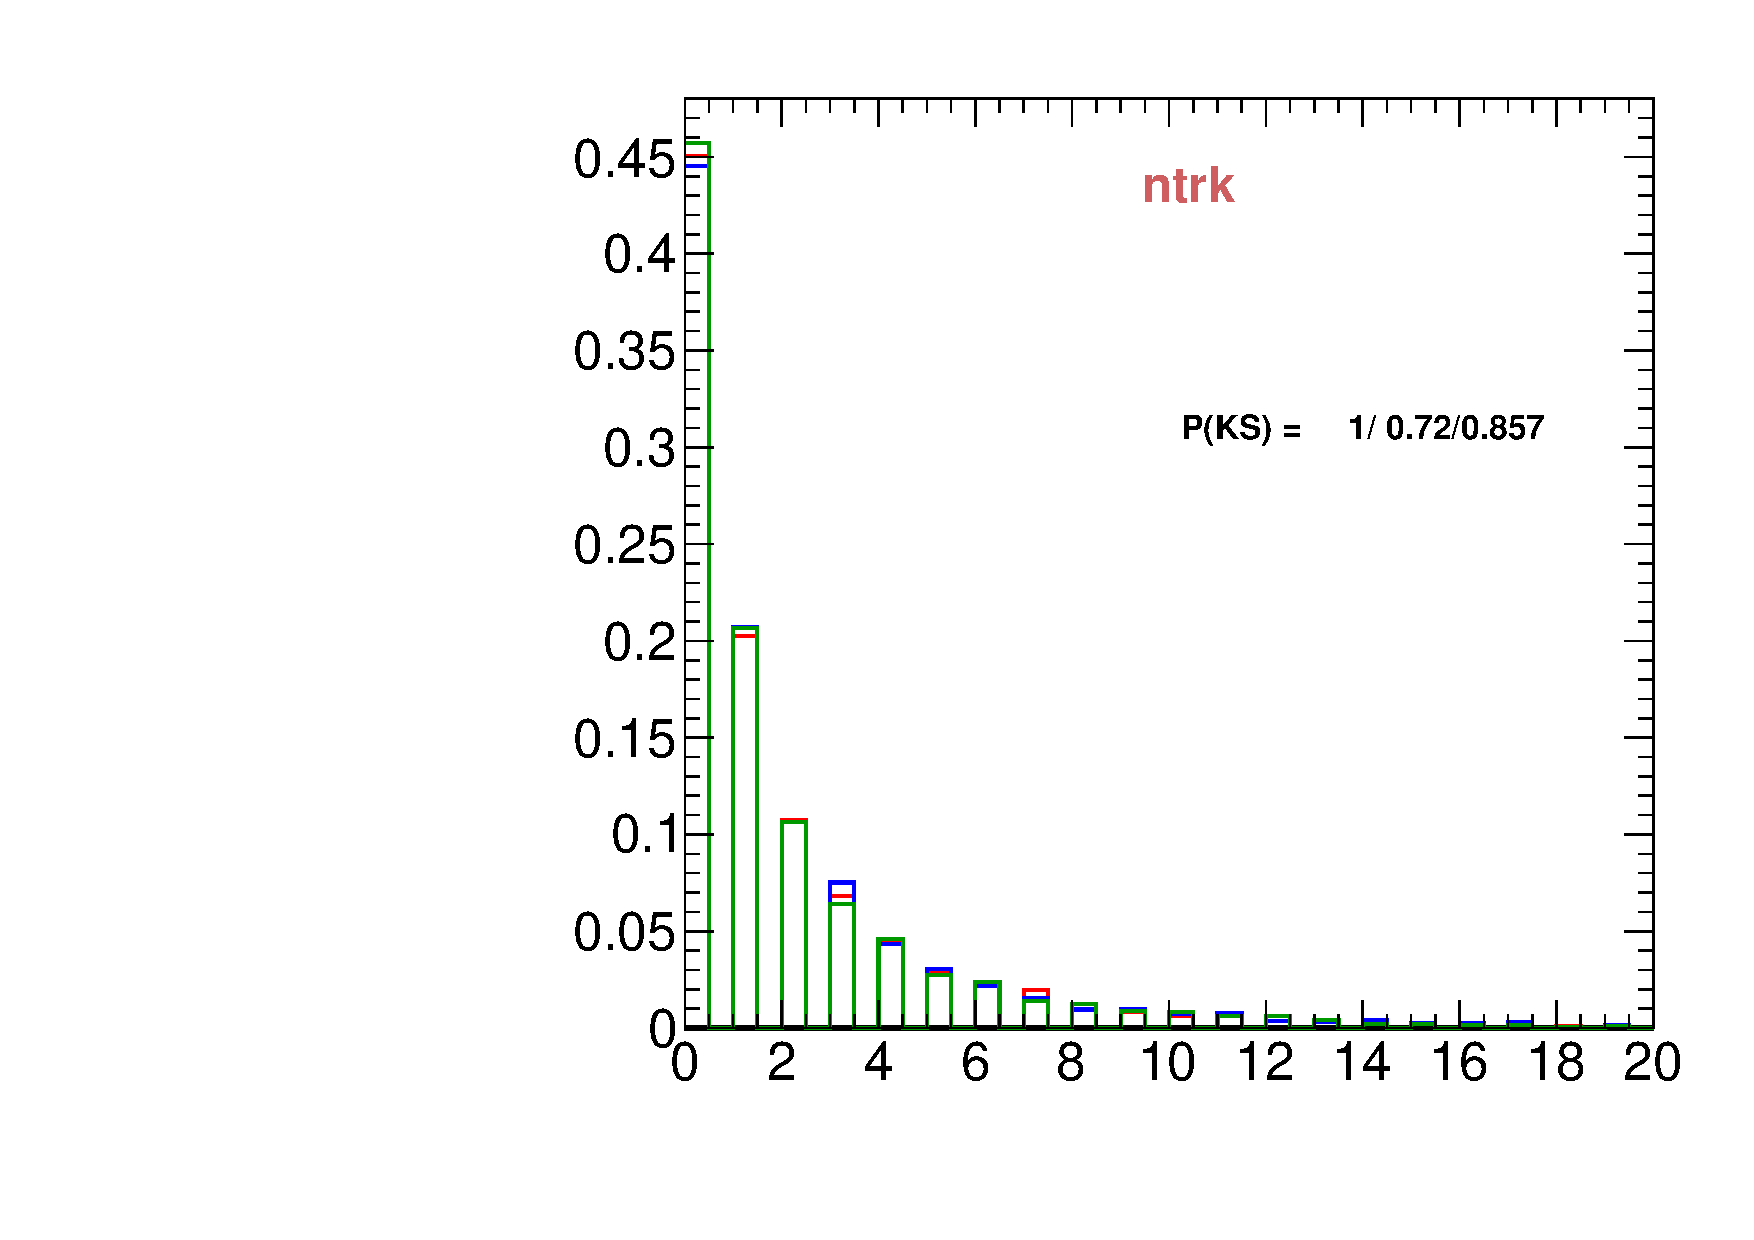
\includegraphics[width=\textwidth]{Figures/VariablesComparison/MC_endcaps_figs_3h/ntrk}
                \label{fig:MC_endcaps_ntrk_3h}
        \end{subfigure}
        \begin{subfigure}[b]{0.2\textwidth}
                \centering
                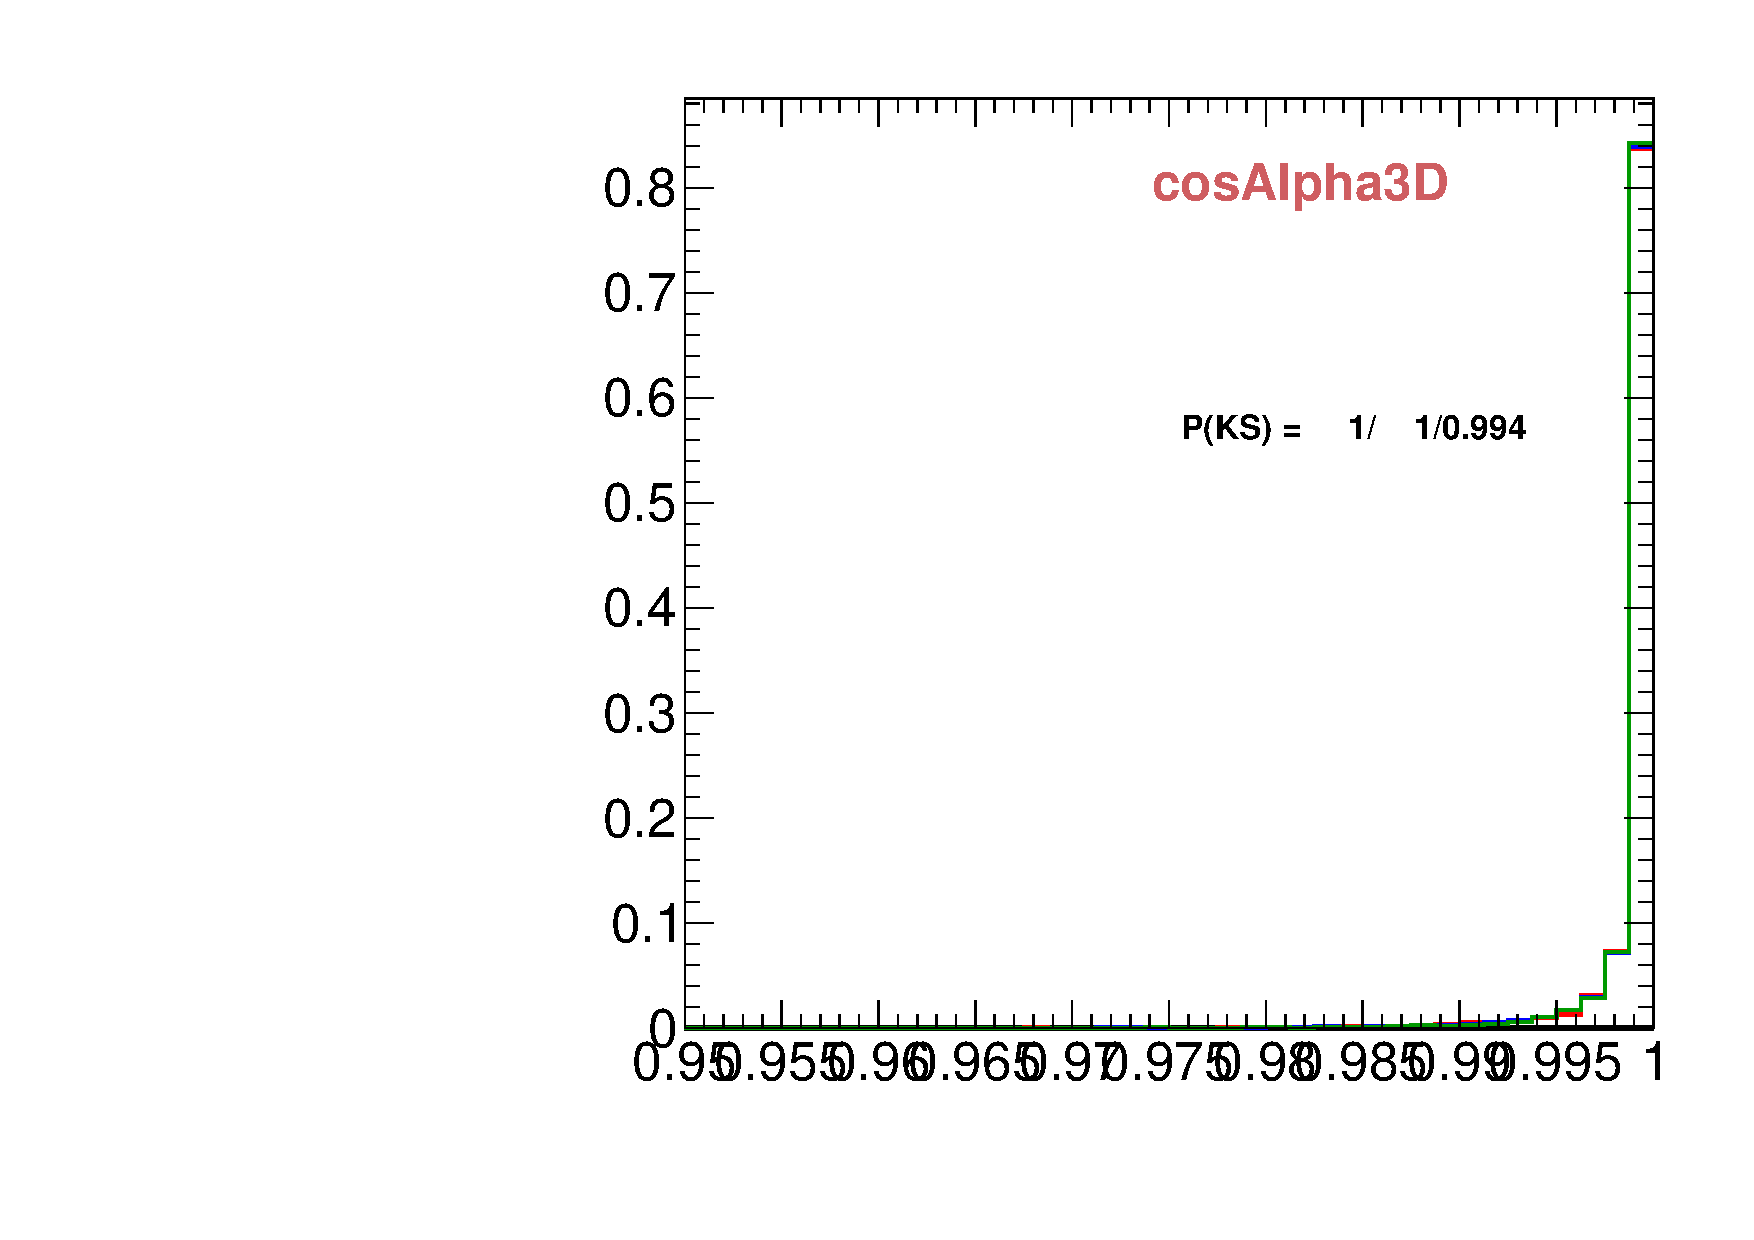
\includegraphics[width=\textwidth]{Figures/VariablesComparison/MC_endcaps_figs_3h/cosAlpha3D}
                \label{fig:MC_endcaps_cosAlpha3D_3h}
        \end{subfigure}
        \begin{subfigure}[b]{0.2\textwidth}
                \centering
                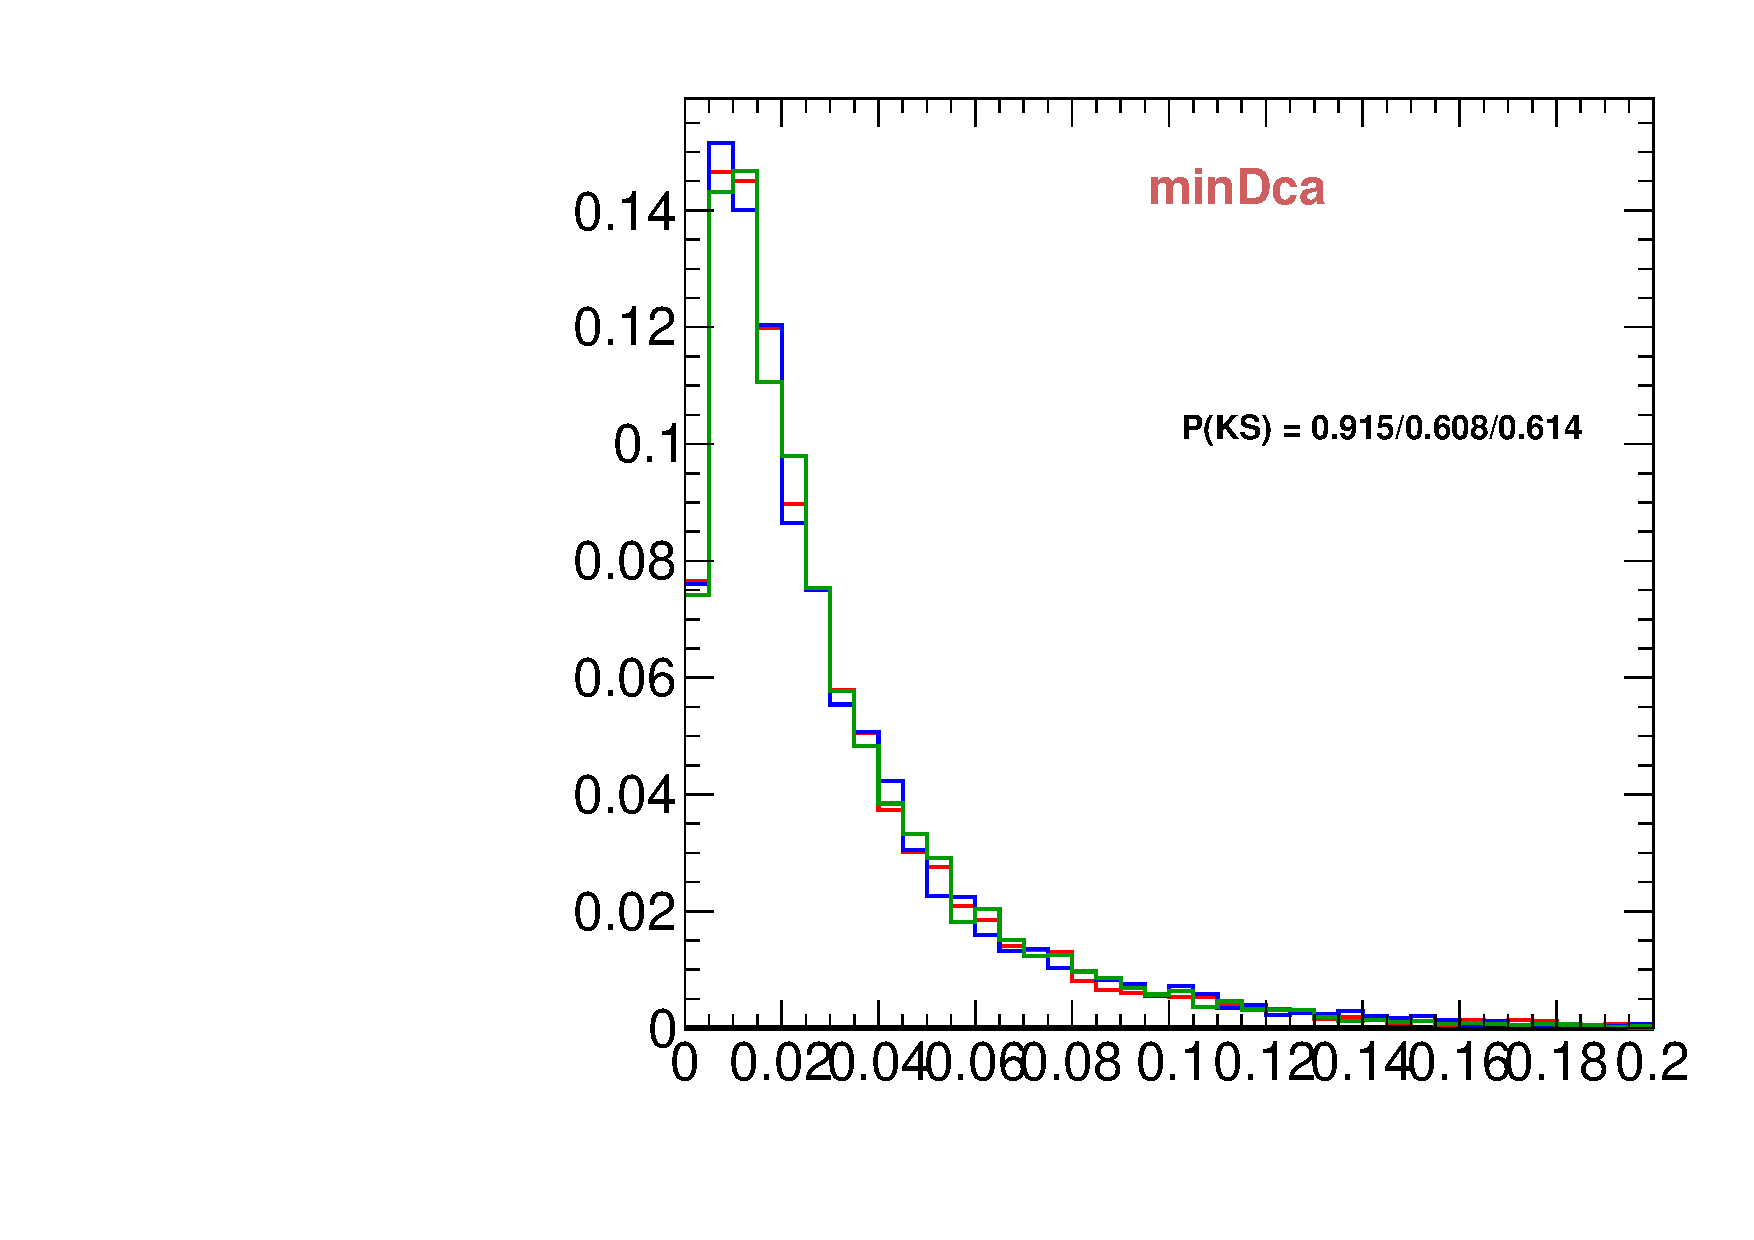
\includegraphics[width=\textwidth]{Figures/VariablesComparison/MC_endcaps_figs_3h/minDca}
                \label{fig:MC_endcaps_minDca_3h}
        \end{subfigure}
        \begin{subfigure}[b]{0.2\textwidth}
                \centering
                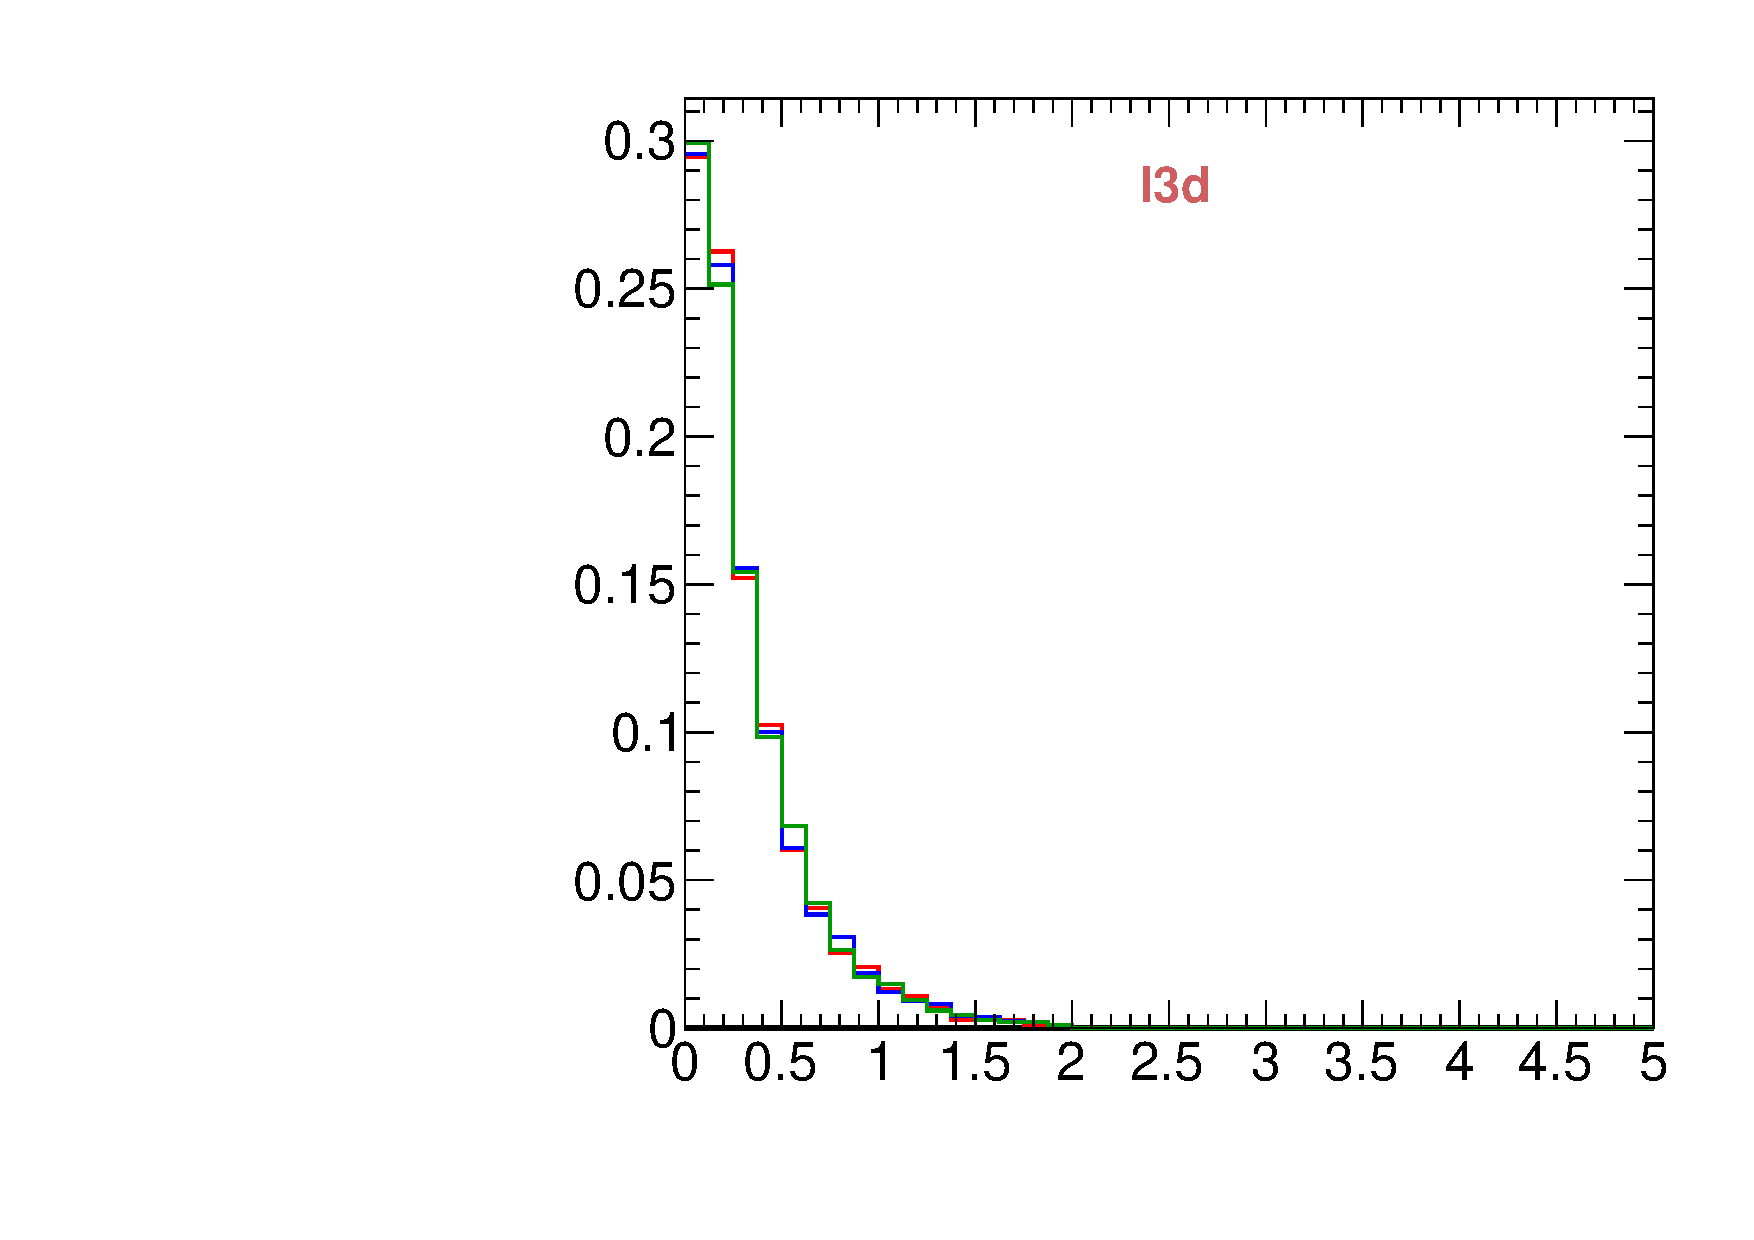
\includegraphics[width=\textwidth]{Figures/VariablesComparison/MC_endcaps_figs_3h/l3d}
                \label{fig:MC_endcaps_l3d_3h}
        \end{subfigure}
        \begin{subfigure}[b]{0.2\textwidth}
                \centering
                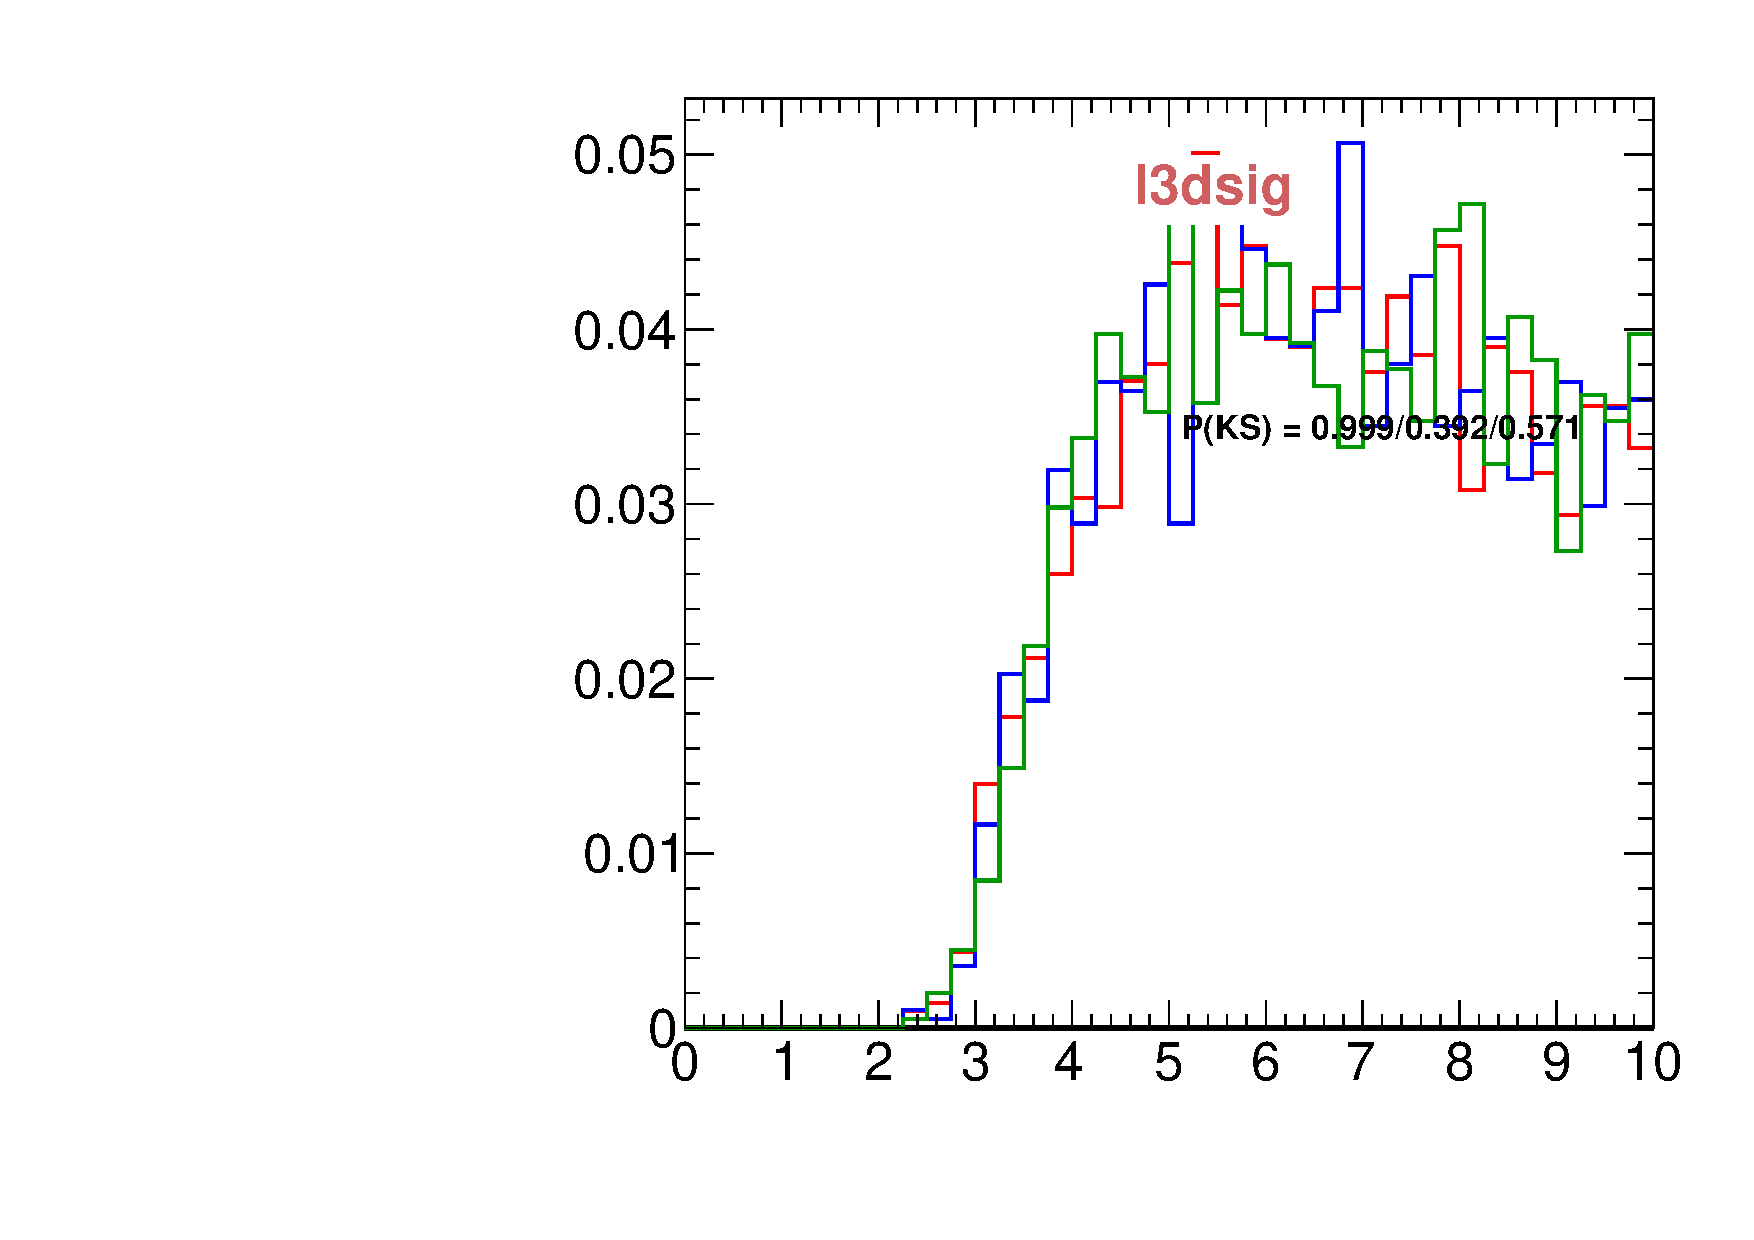
\includegraphics[width=\textwidth]{Figures/VariablesComparison/MC_endcaps_figs_3h/l3dsig}
                \label{fig:MC_endcaps_l3dsig_3h}
        \end{subfigure}
        \begin{subfigure}[b]{0.2\textwidth}
                \centering
                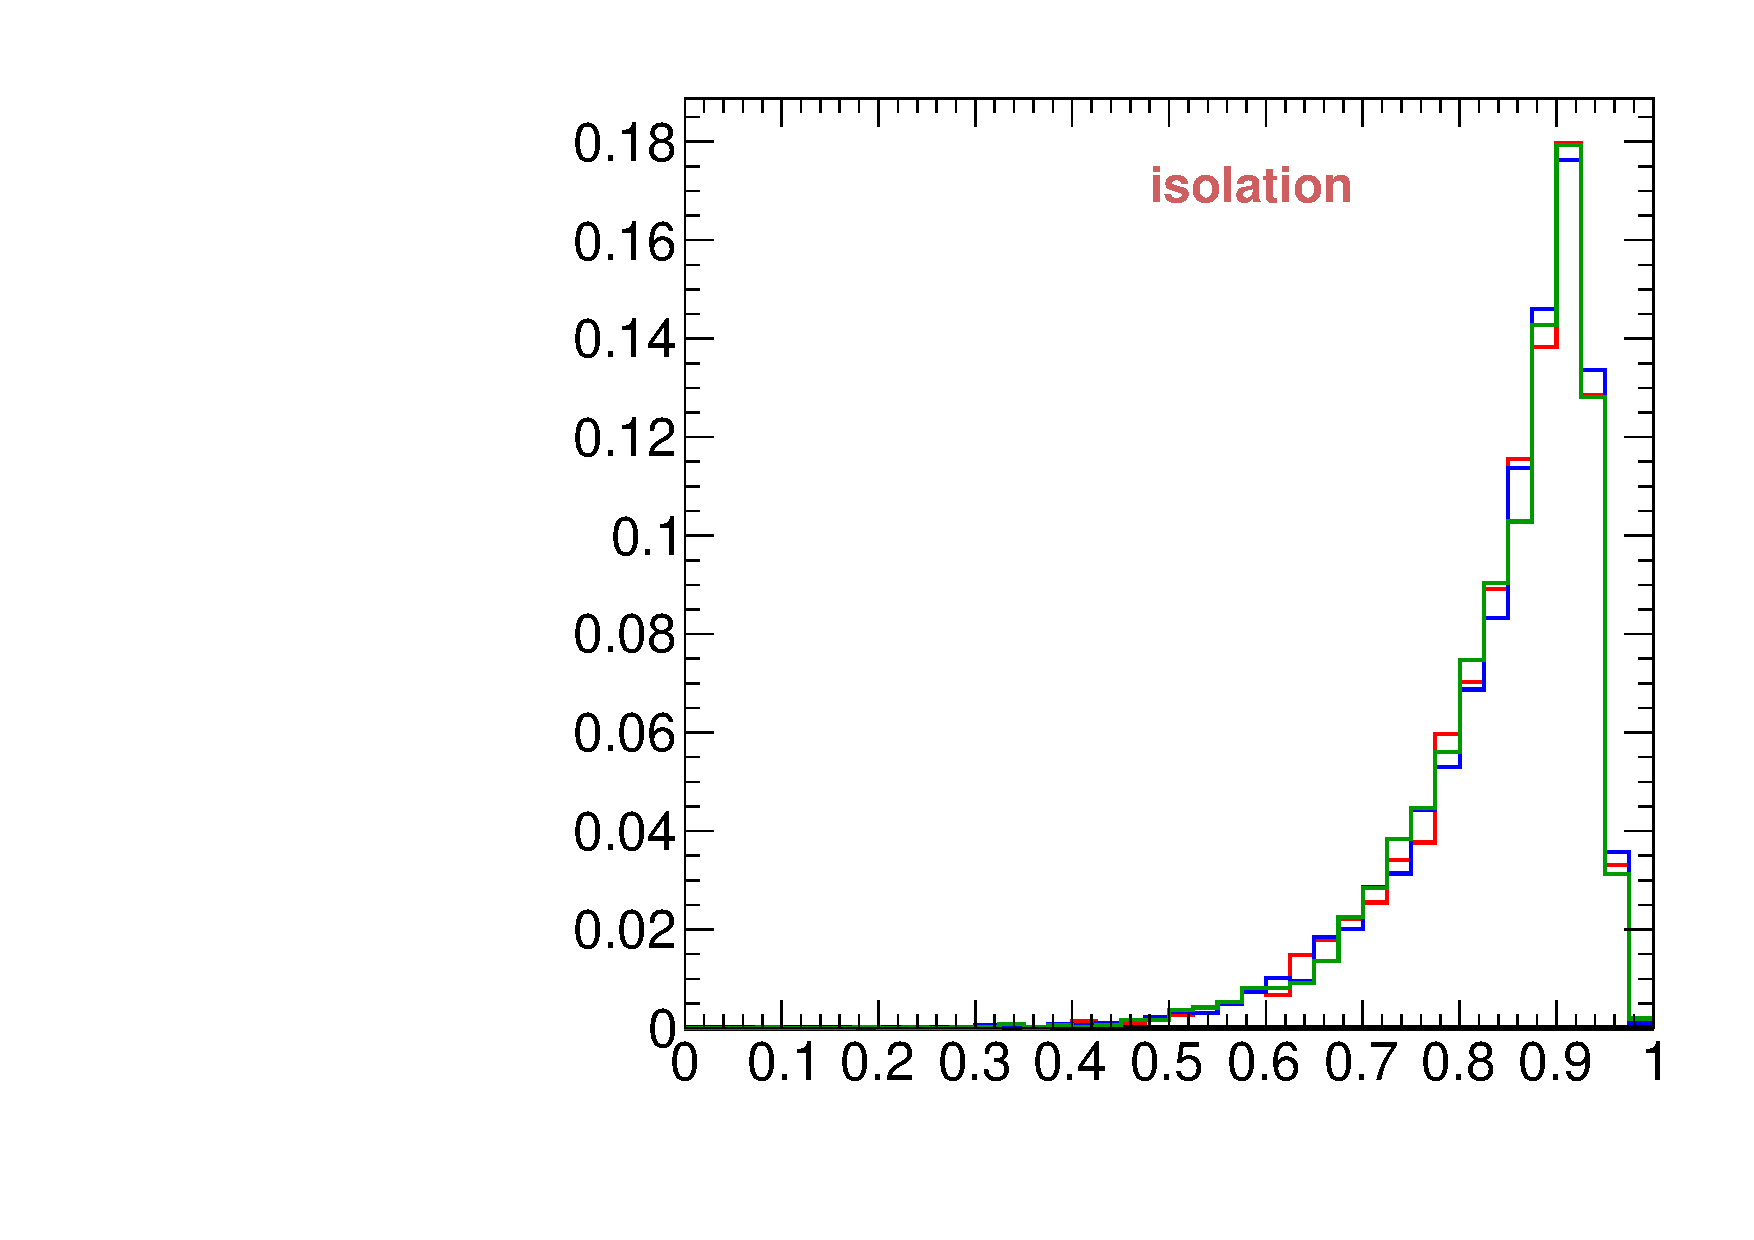
\includegraphics[width=\textwidth]{Figures/VariablesComparison/MC_endcaps_figs_3h/isolation}
                \label{fig:MC_endcaps_isolation_3h}
        \end{subfigure}
        \begin{subfigure}[b]{0.2\textwidth}
                \centering
                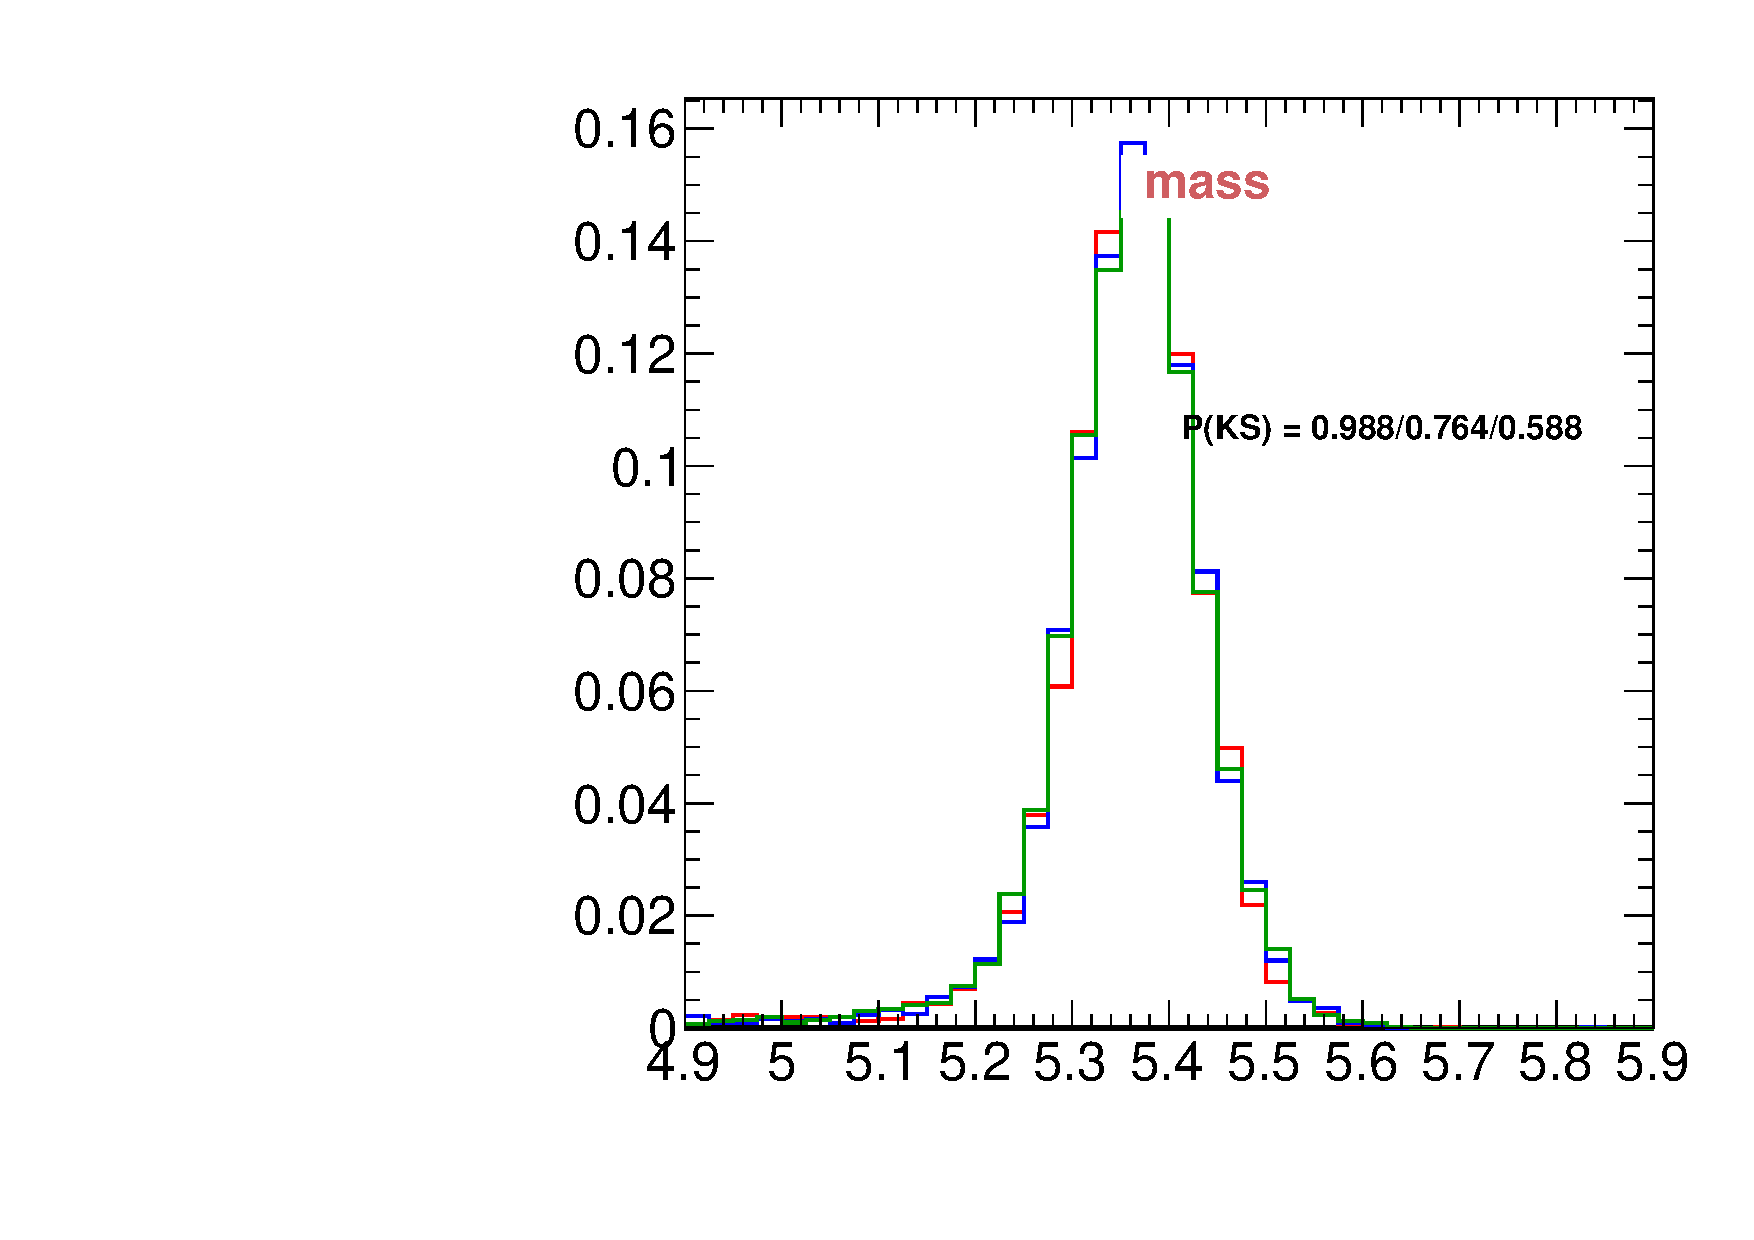
\includegraphics[width=\textwidth]{Figures/VariablesComparison/MC_endcaps_figs_3h/mass}
                \label{fig:MC_endcaps_mass_3h}
        \end{subfigure}
        \begin{subfigure}[b]{0.2\textwidth}
                \centering
                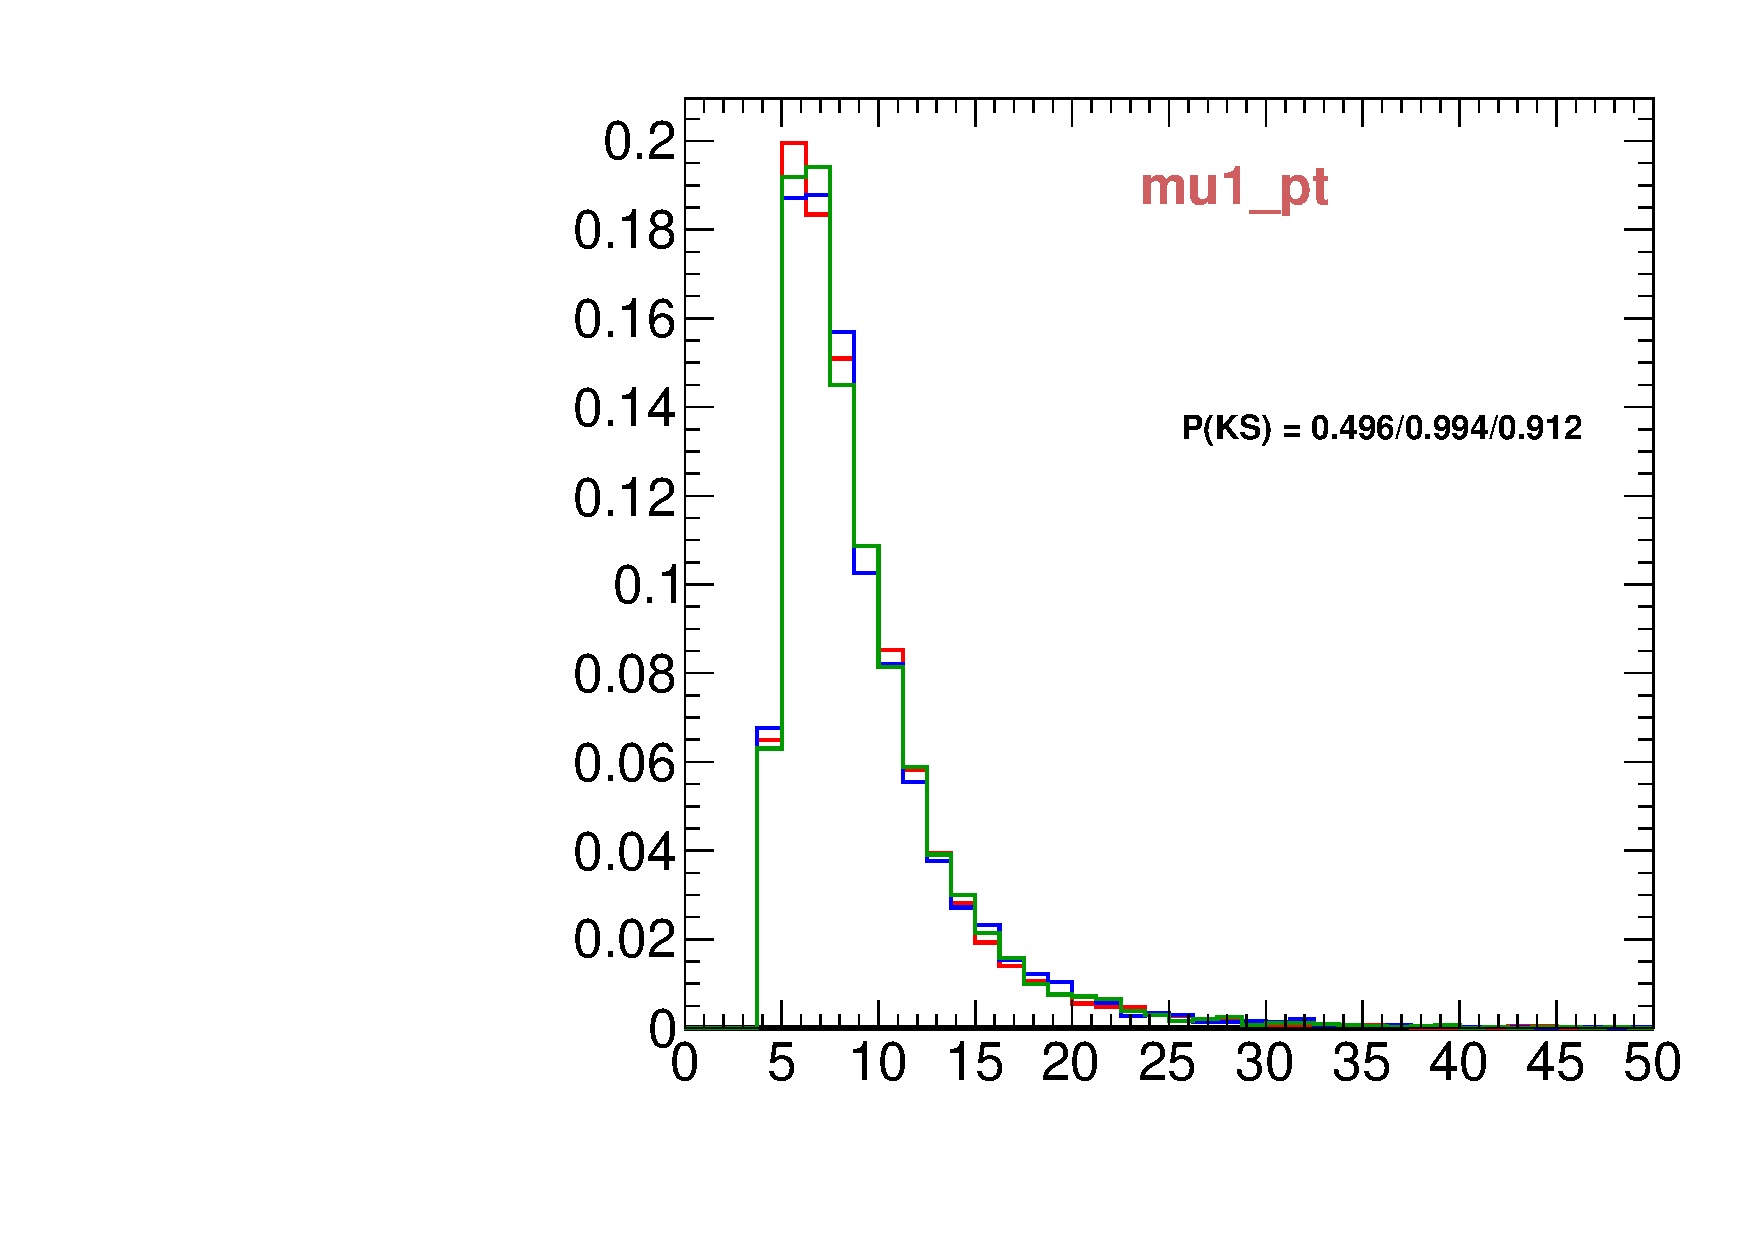
\includegraphics[width=\textwidth]{Figures/VariablesComparison/MC_endcaps_figs_3h/mu1_pt}
                \label{fig:MC_endcaps_mu1_pt_3h}
        \end{subfigure}
        \begin{subfigure}[b]{0.2\textwidth}
                \centering
                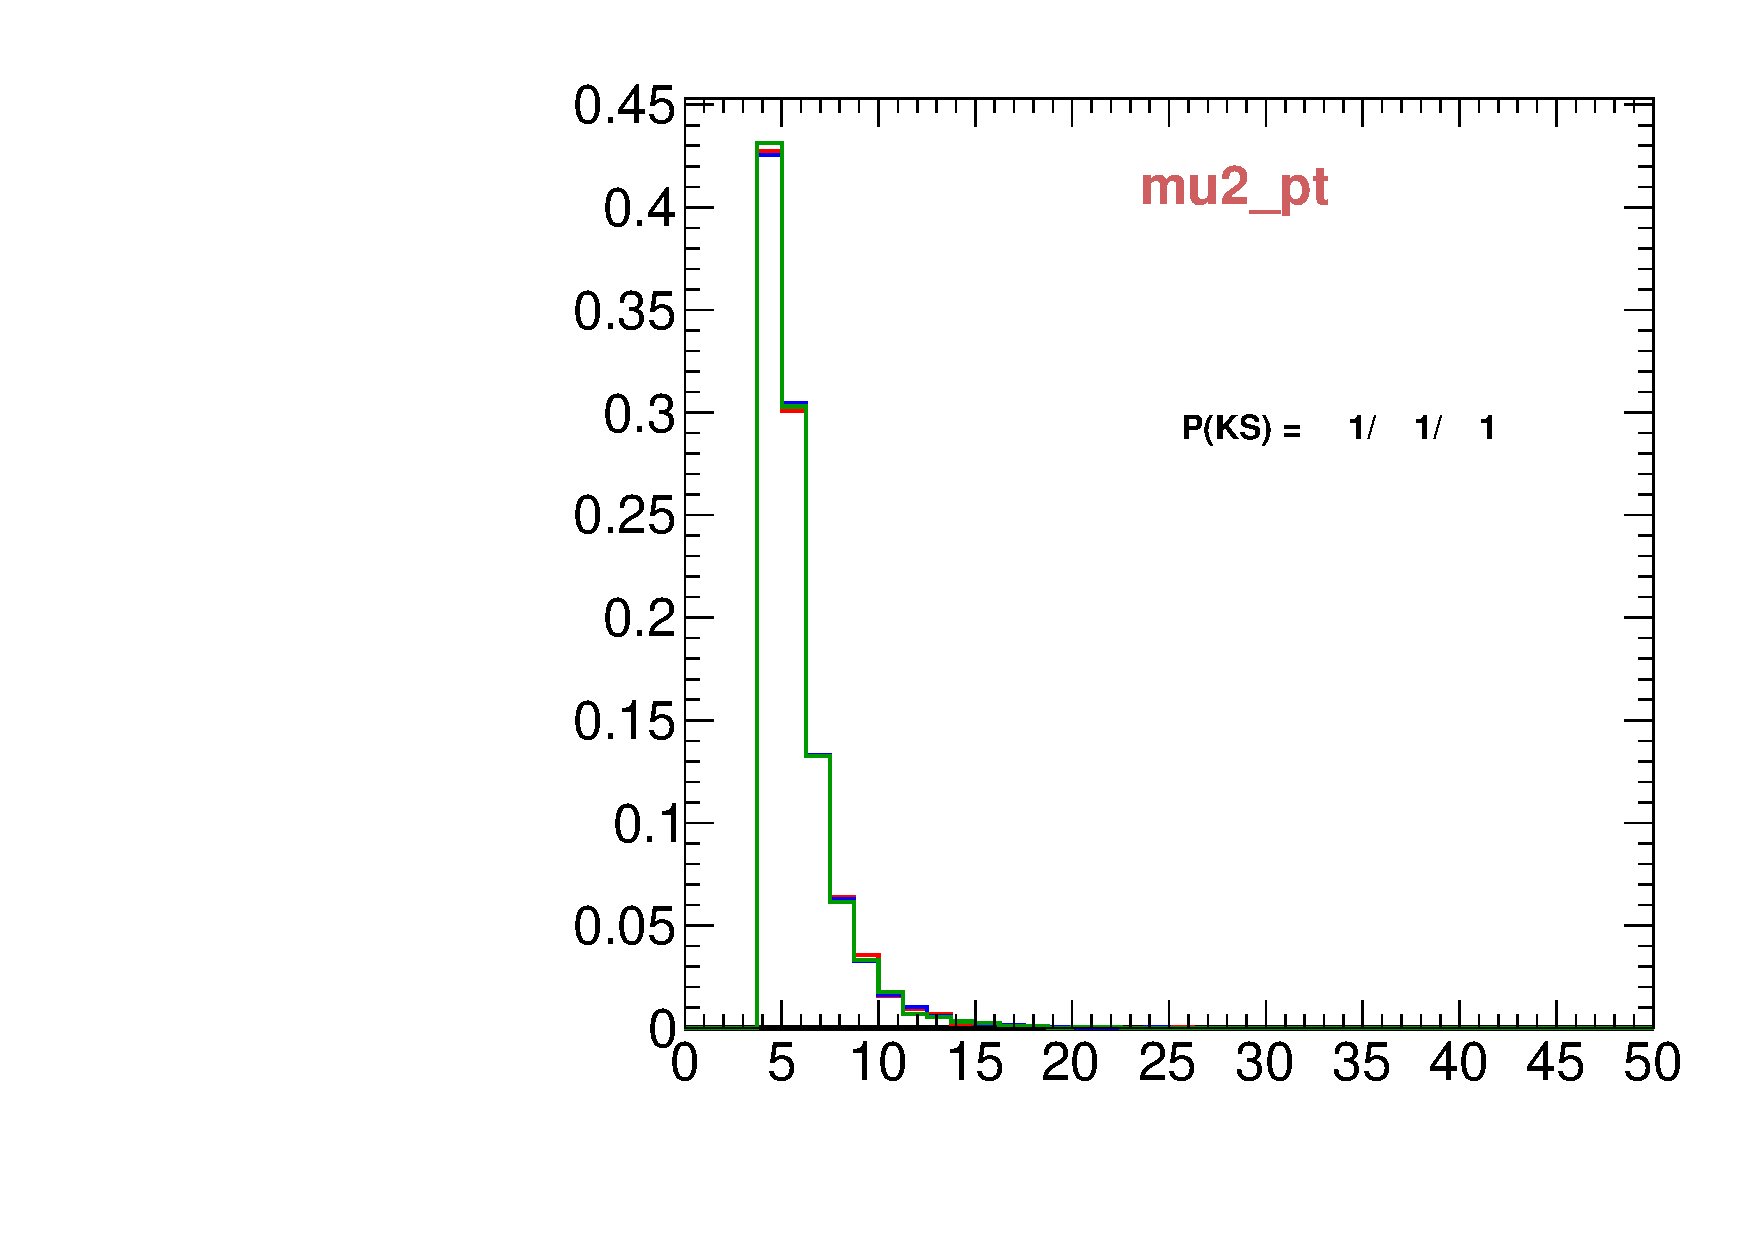
\includegraphics[width=\textwidth]{Figures/VariablesComparison/MC_endcaps_figs_3h/mu2_pt}
                \label{fig:MC_endcaps_mu2_pt_3h}
        \end{subfigure}
        \begin{subfigure}[b]{0.2\textwidth}
                \centering
                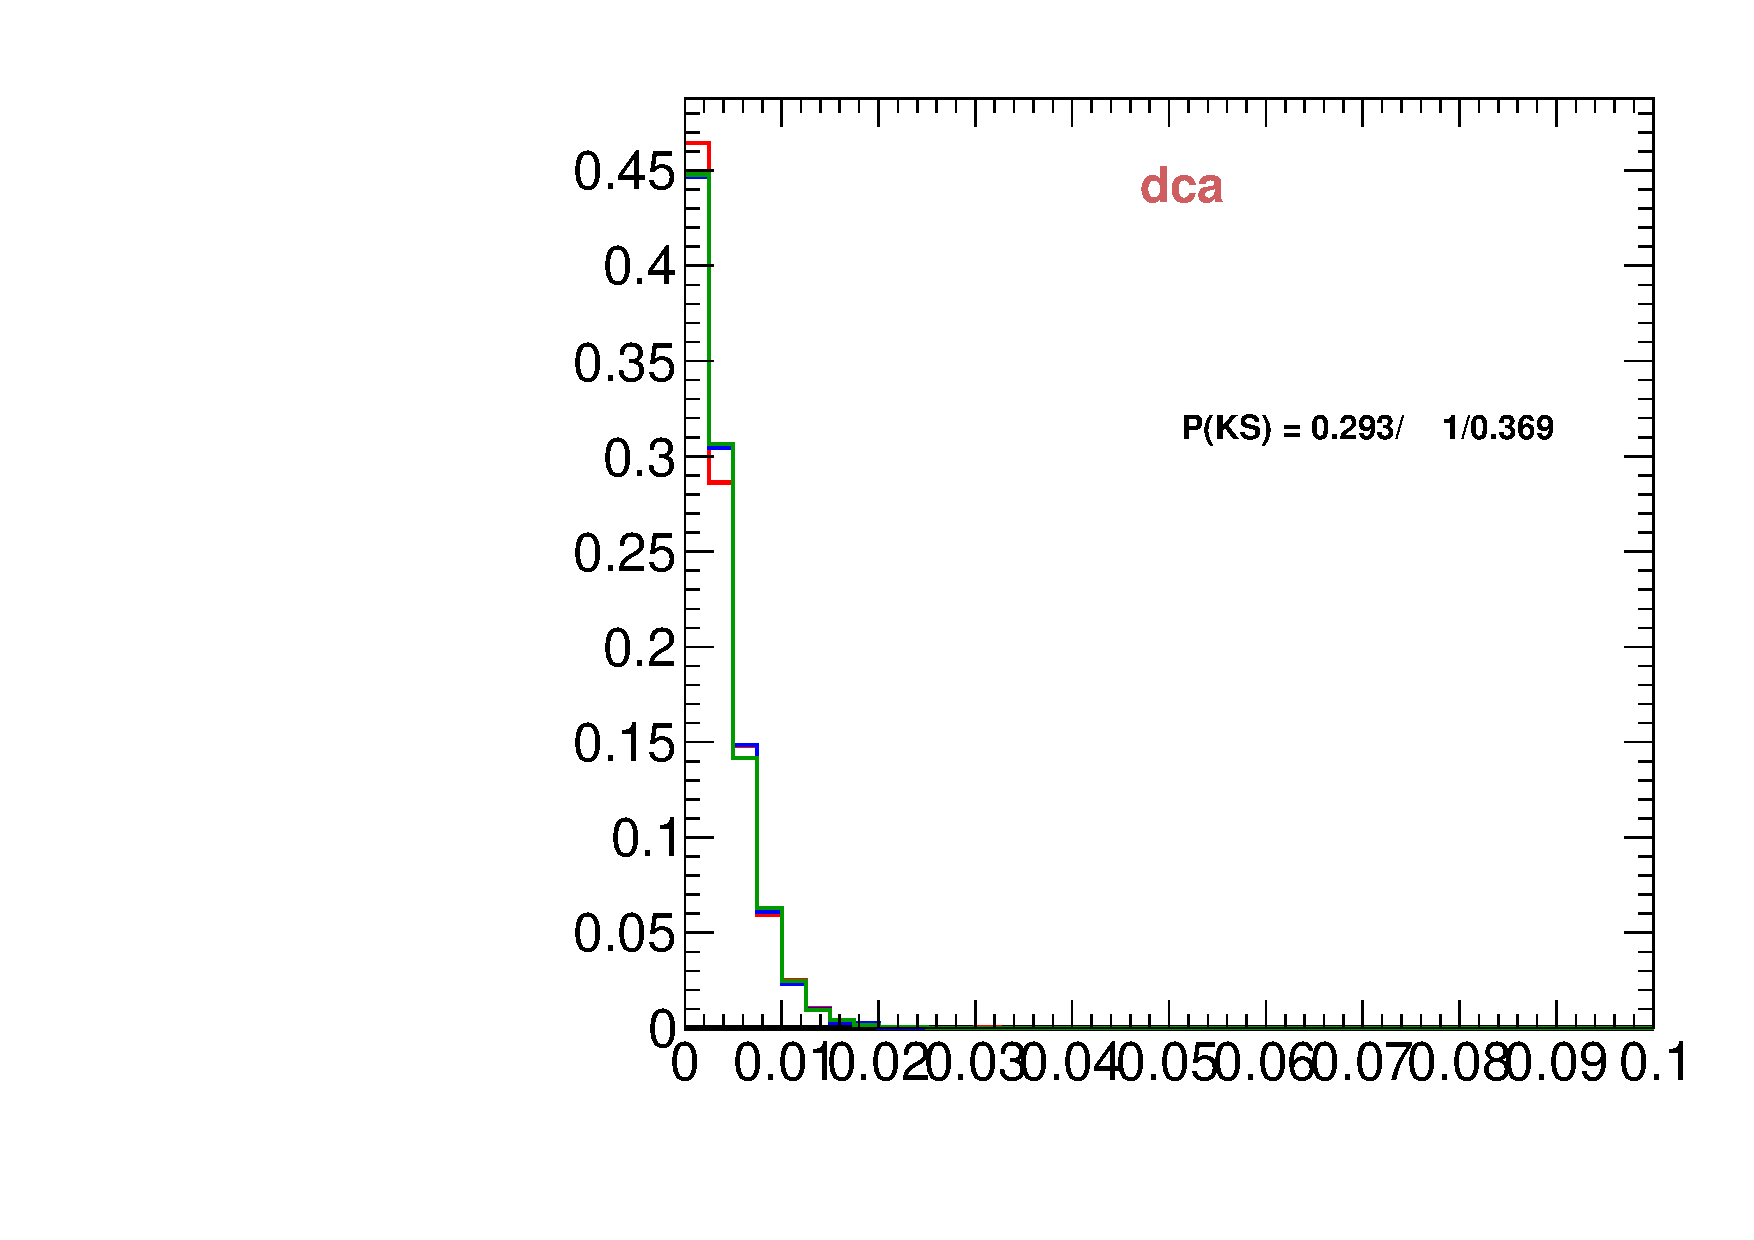
\includegraphics[width=\textwidth]{Figures/VariablesComparison/MC_endcaps_figs_3h/dca}
                \label{fig:MC_endcaps_dca_3h}
        \end{subfigure}
        \begin{subfigure}[b]{0.2\textwidth}
                \centering
                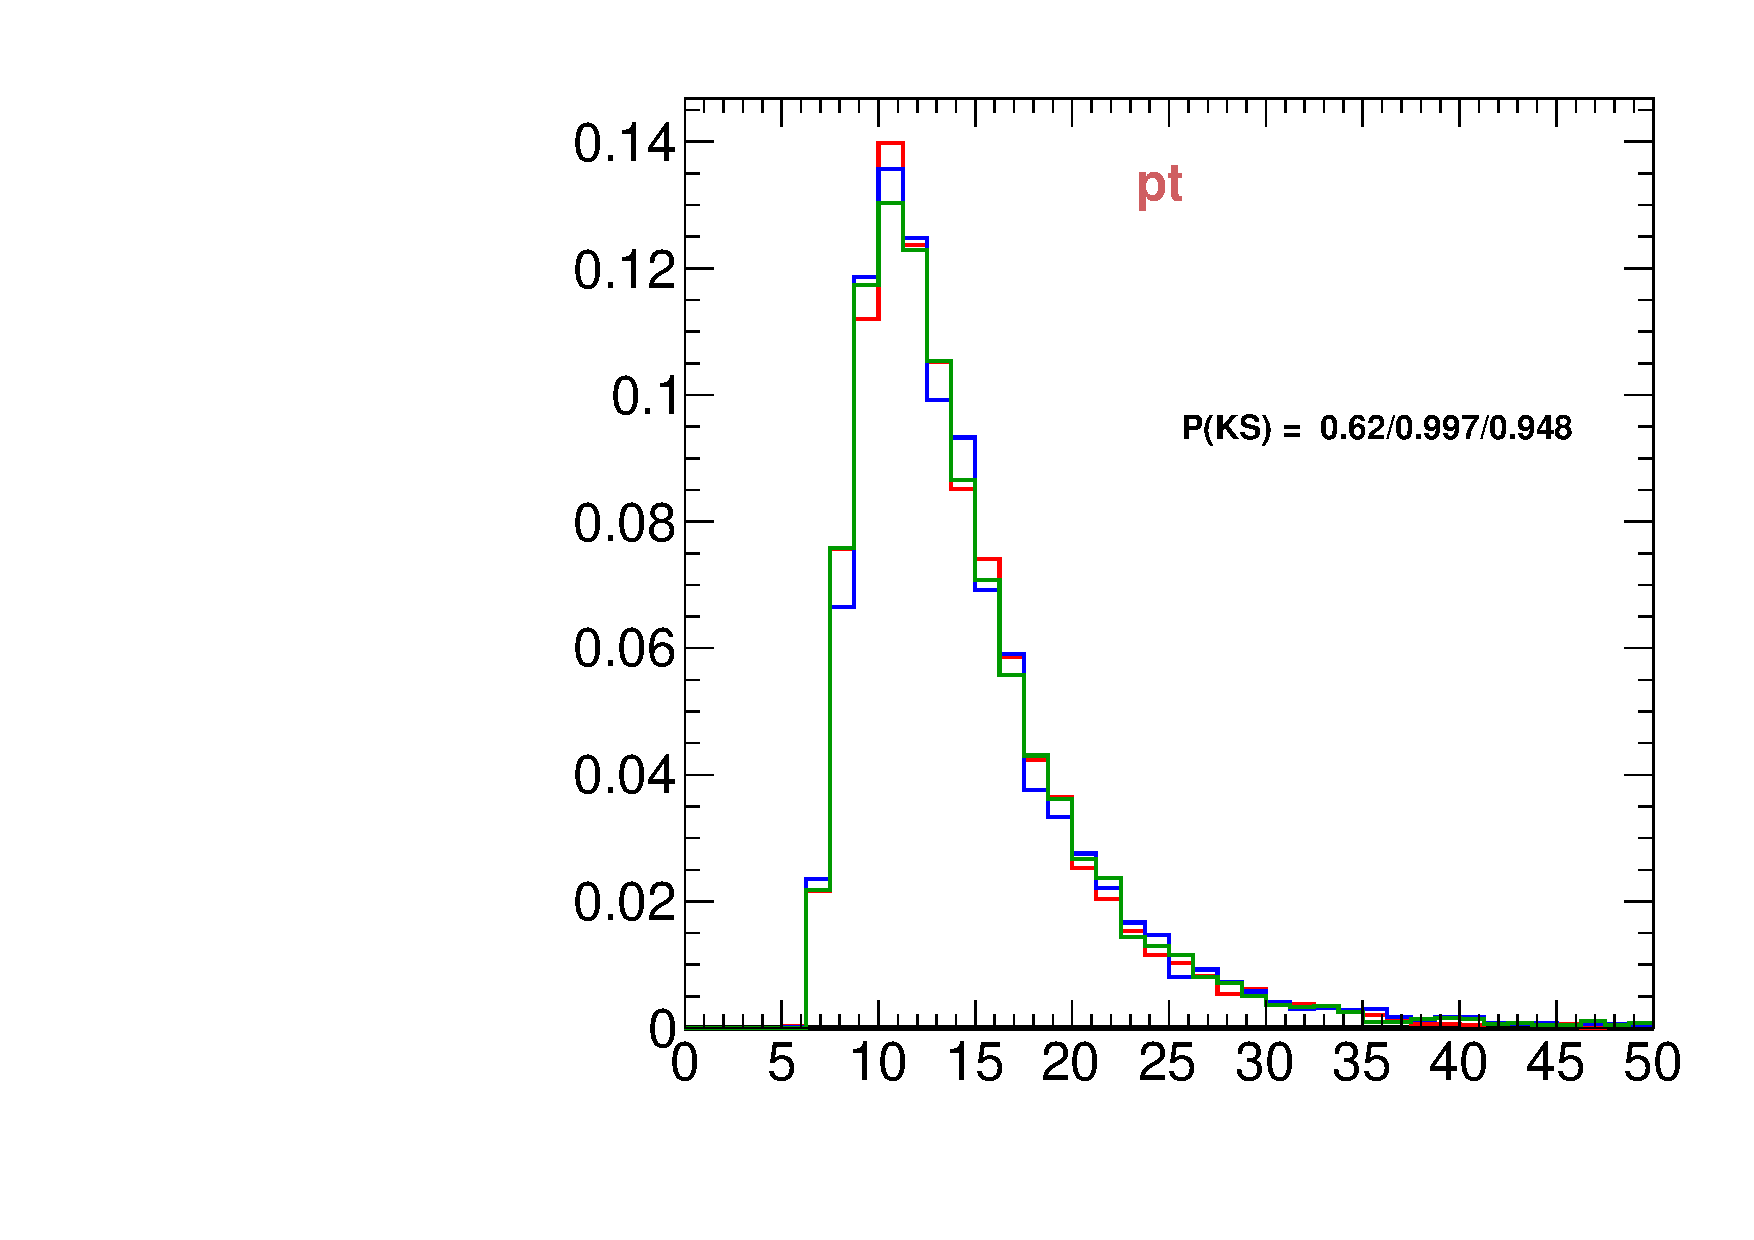
\includegraphics[width=\textwidth]{Figures/VariablesComparison/MC_endcaps_figs_3h/pt}
                \label{fig:MC_endcaps_pt_3h}
        \end{subfigure}
        \begin{subfigure}[b]{0.2\textwidth}
                \centering
                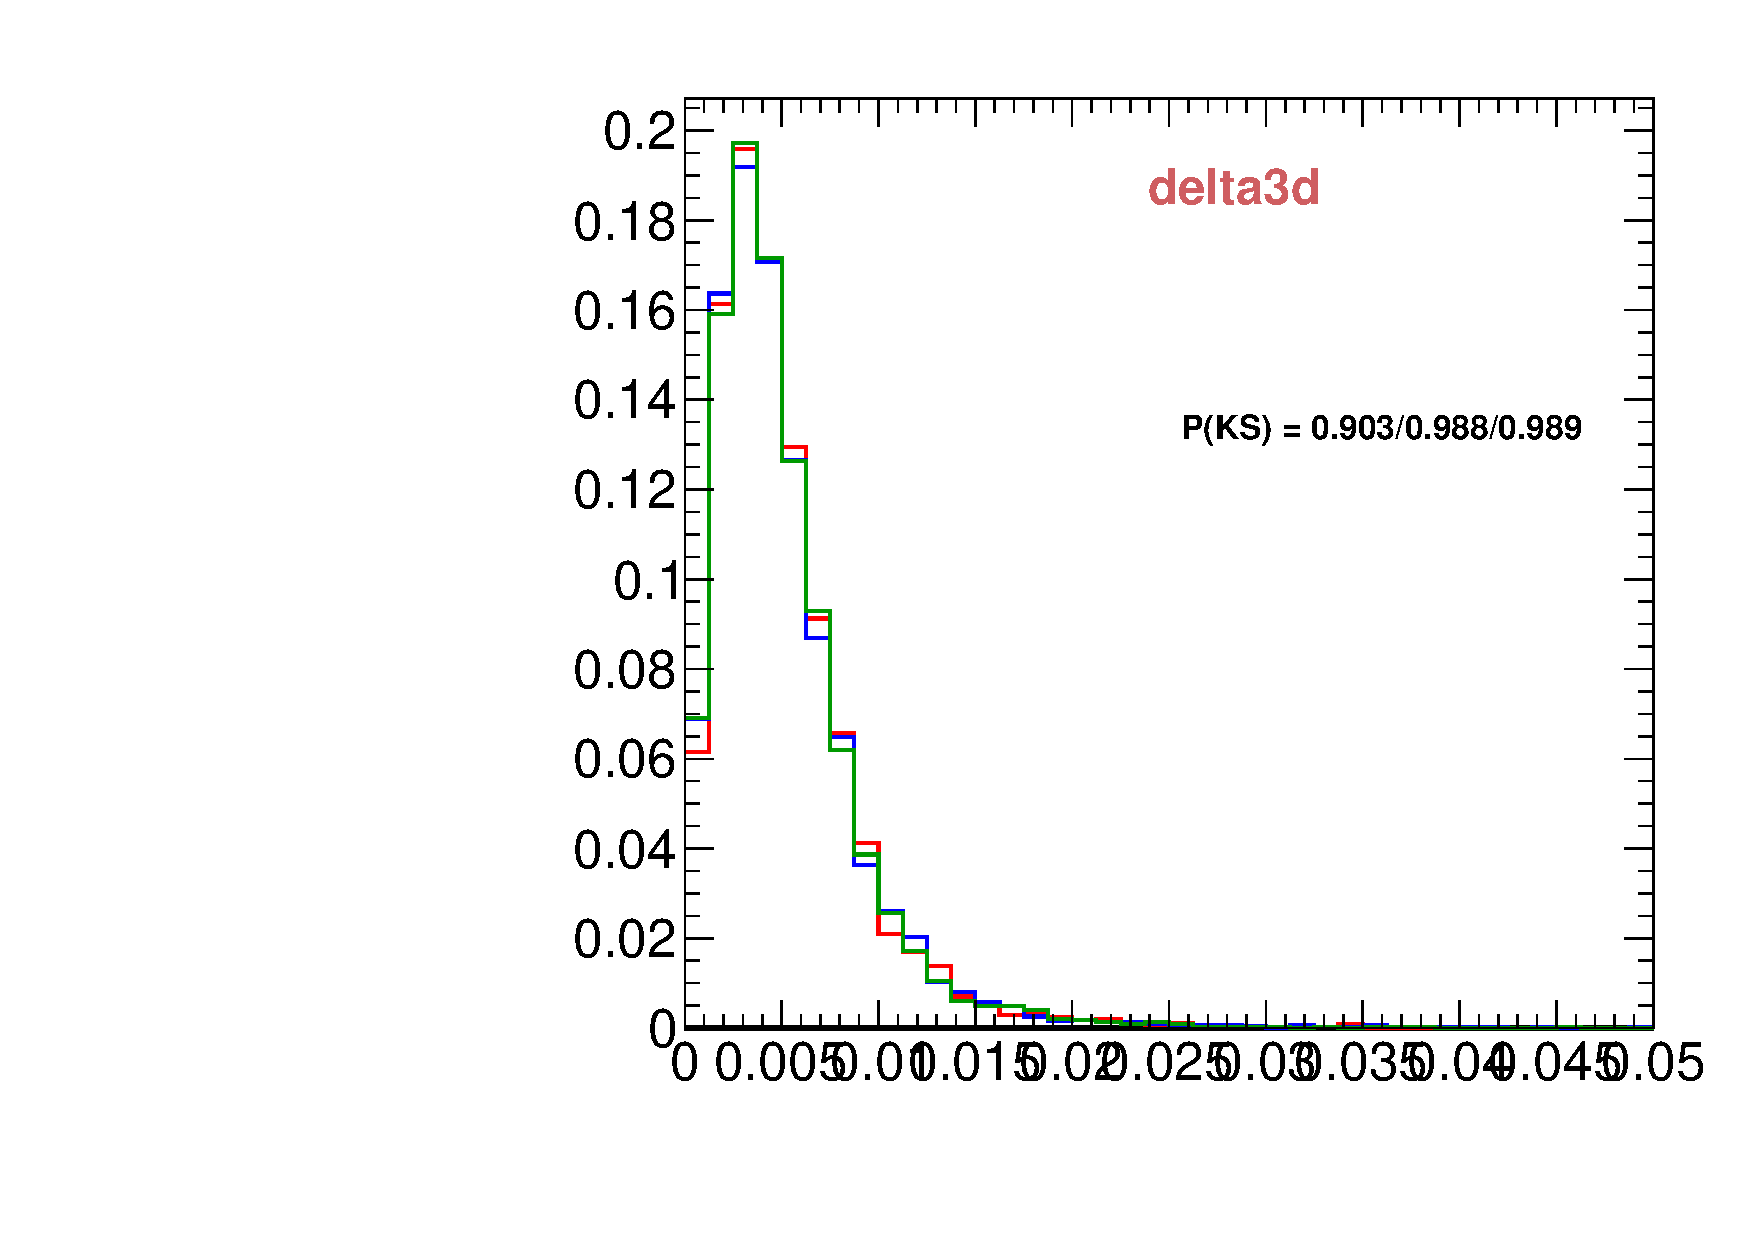
\includegraphics[width=\textwidth]{Figures/VariablesComparison/MC_endcaps_figs_3h/delta3d}
                \label{fig:MC_endcaps_delta3d_3h}
        \end{subfigure}
        \begin{subfigure}[b]{0.2\textwidth}
                \centering
                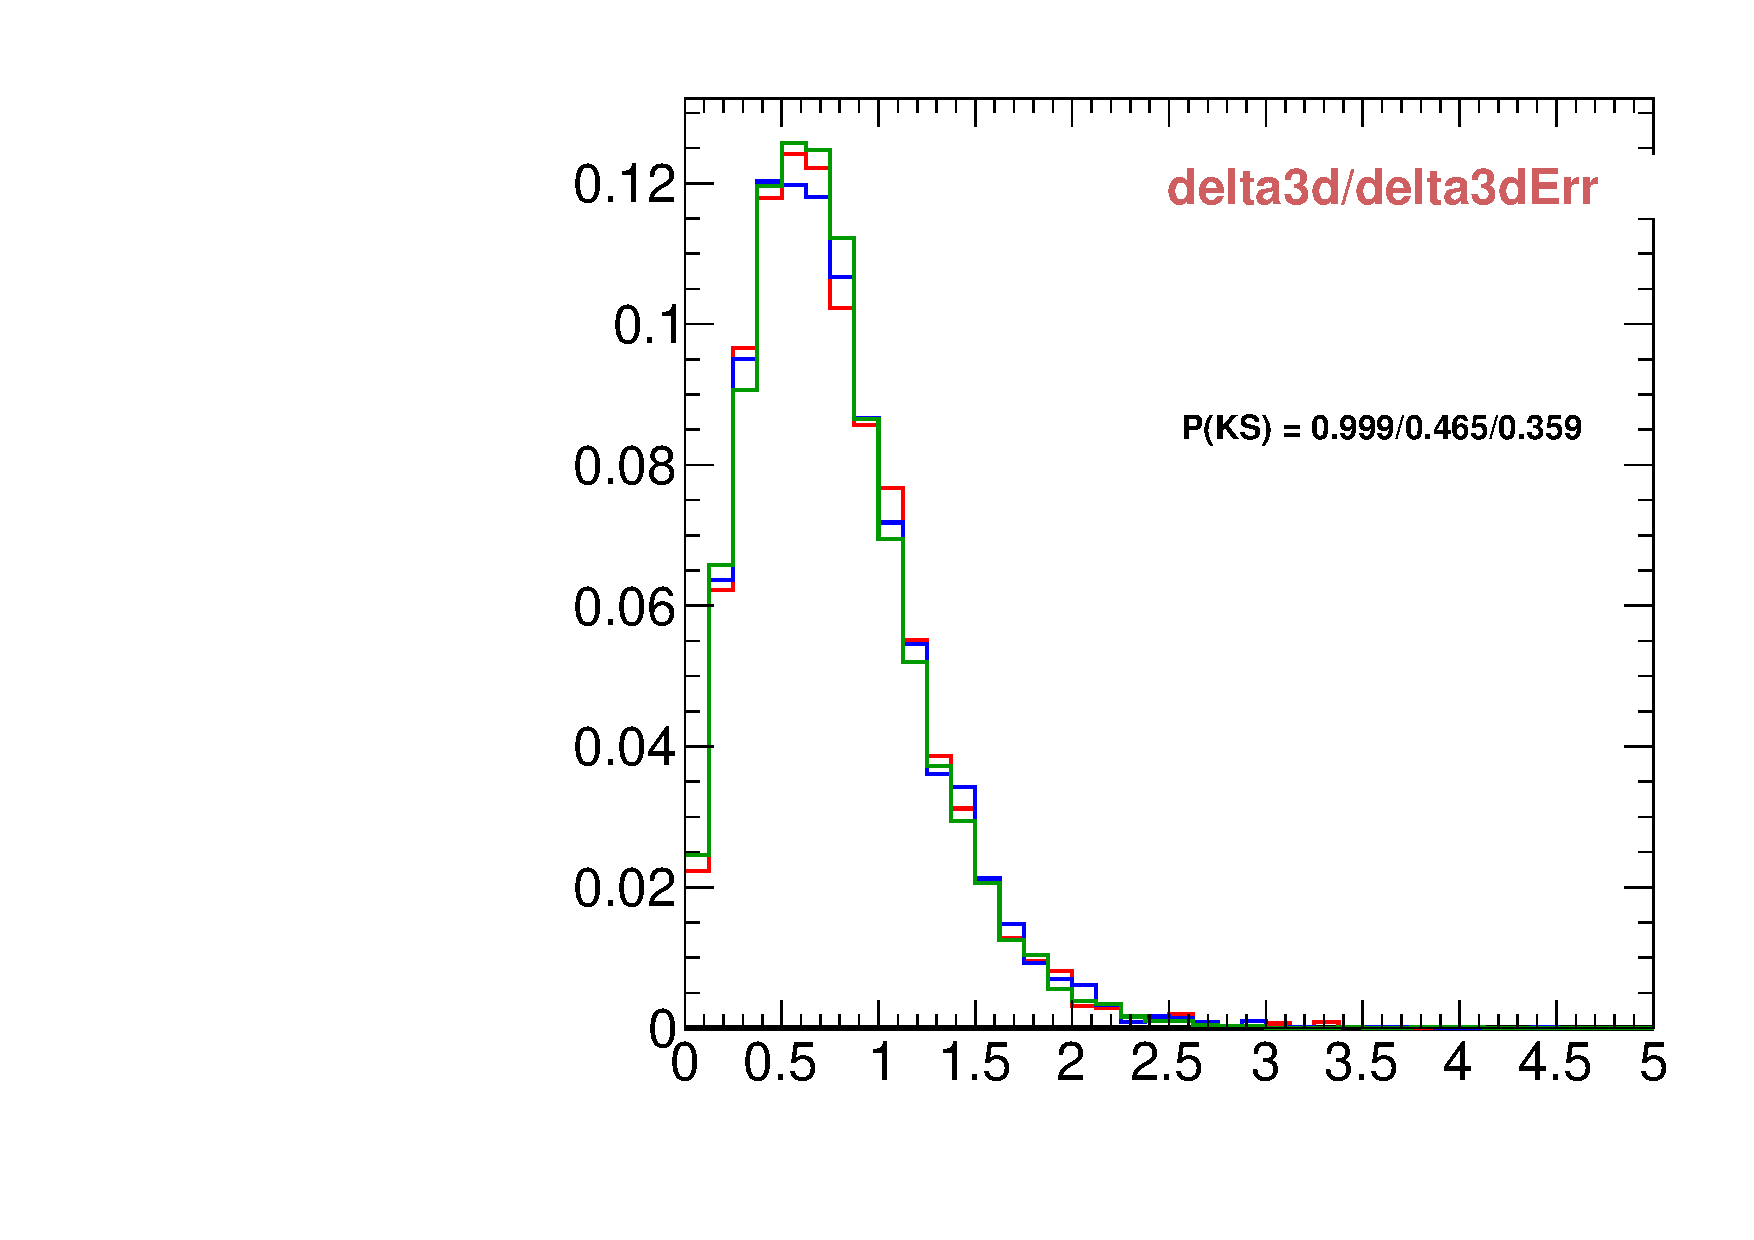
\includegraphics[width=\textwidth]{Figures/VariablesComparison/MC_endcaps_figs_3h/delta3dErr}
                \label{fig:MC_endcaps_delta3d/delta3dErr_3h}
        \end{subfigure}
        \begin{subfigure}[b]{0.2\textwidth}
                \centering
                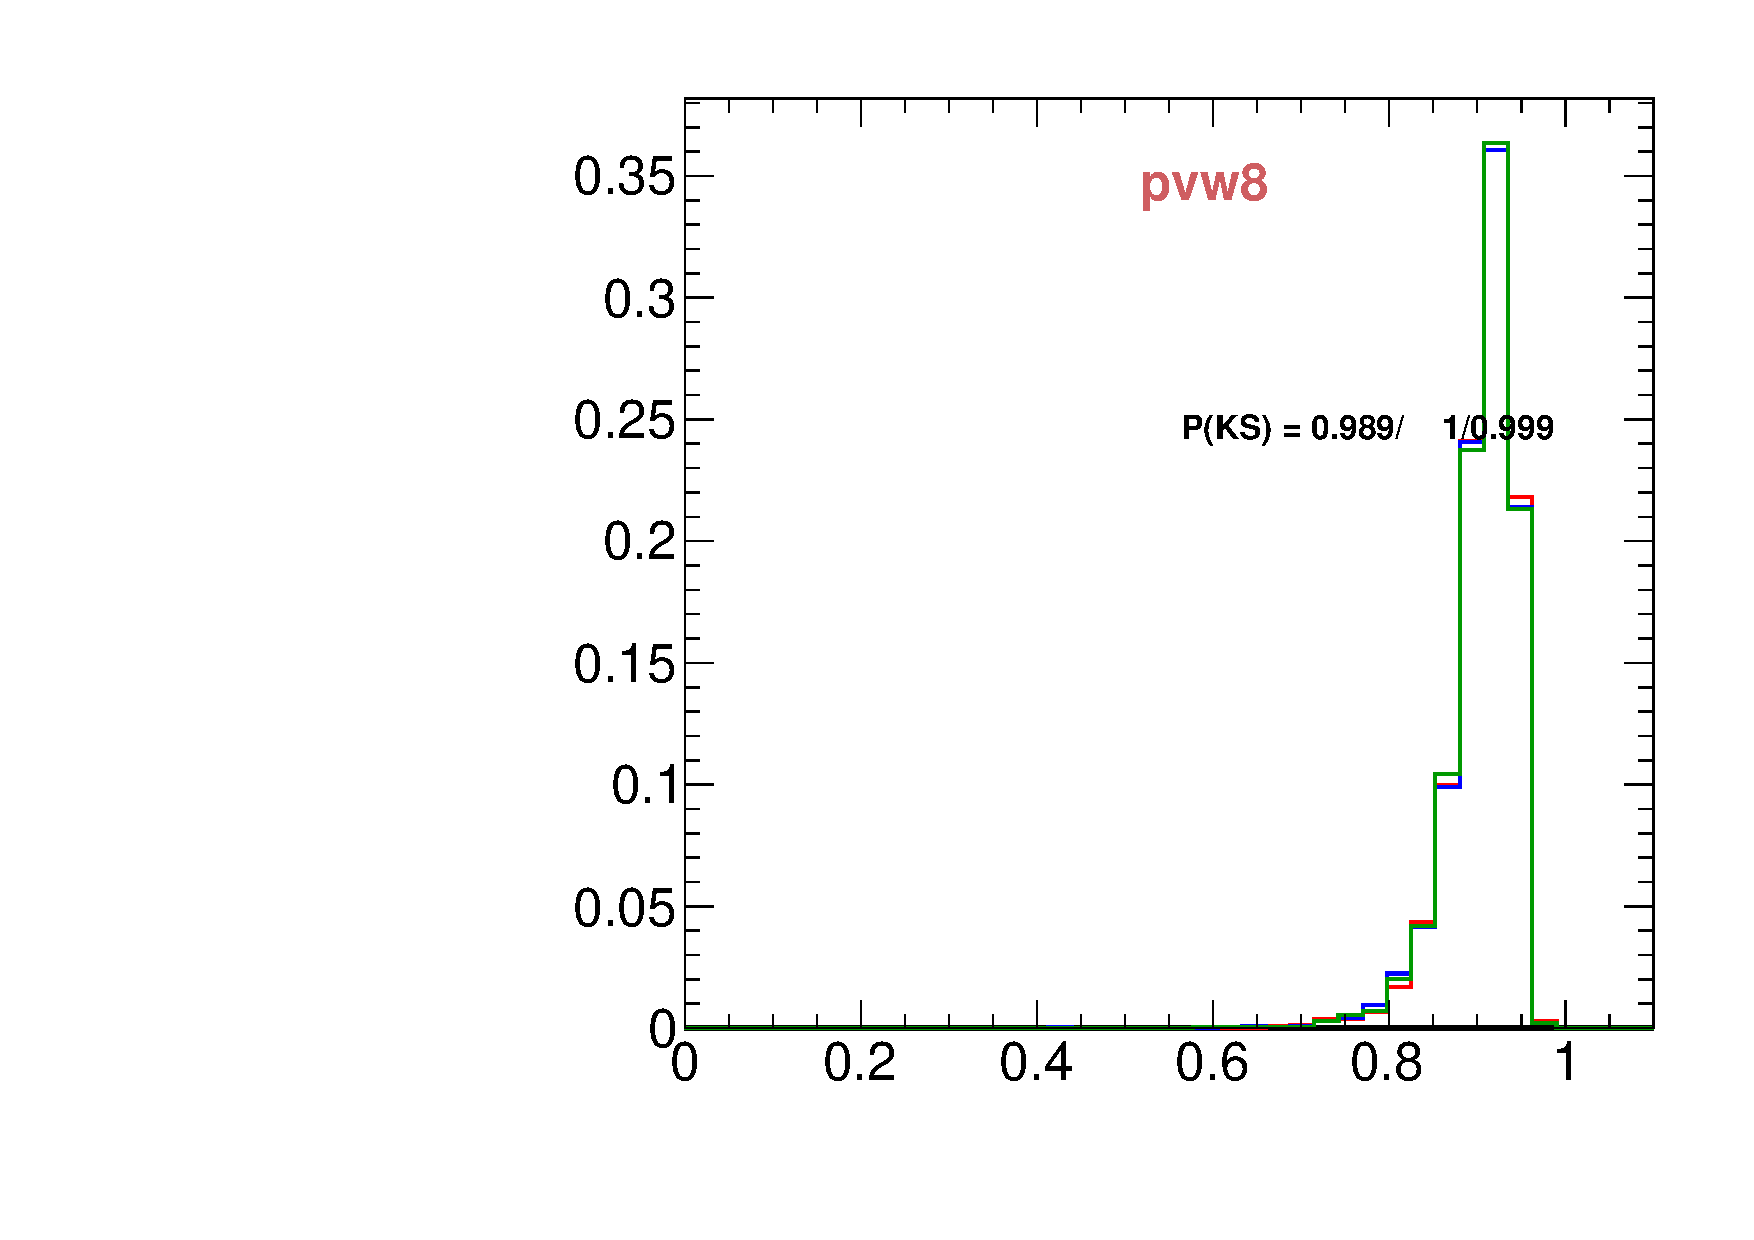
\includegraphics[width=\textwidth]{Figures/VariablesComparison/MC_endcaps_figs_3h/pvw8}
                \label{fig:MC_endcaps_pvw8_3h}
        \end{subfigure}
        \begin{subfigure}[b]{0.2\textwidth}
                \centering
                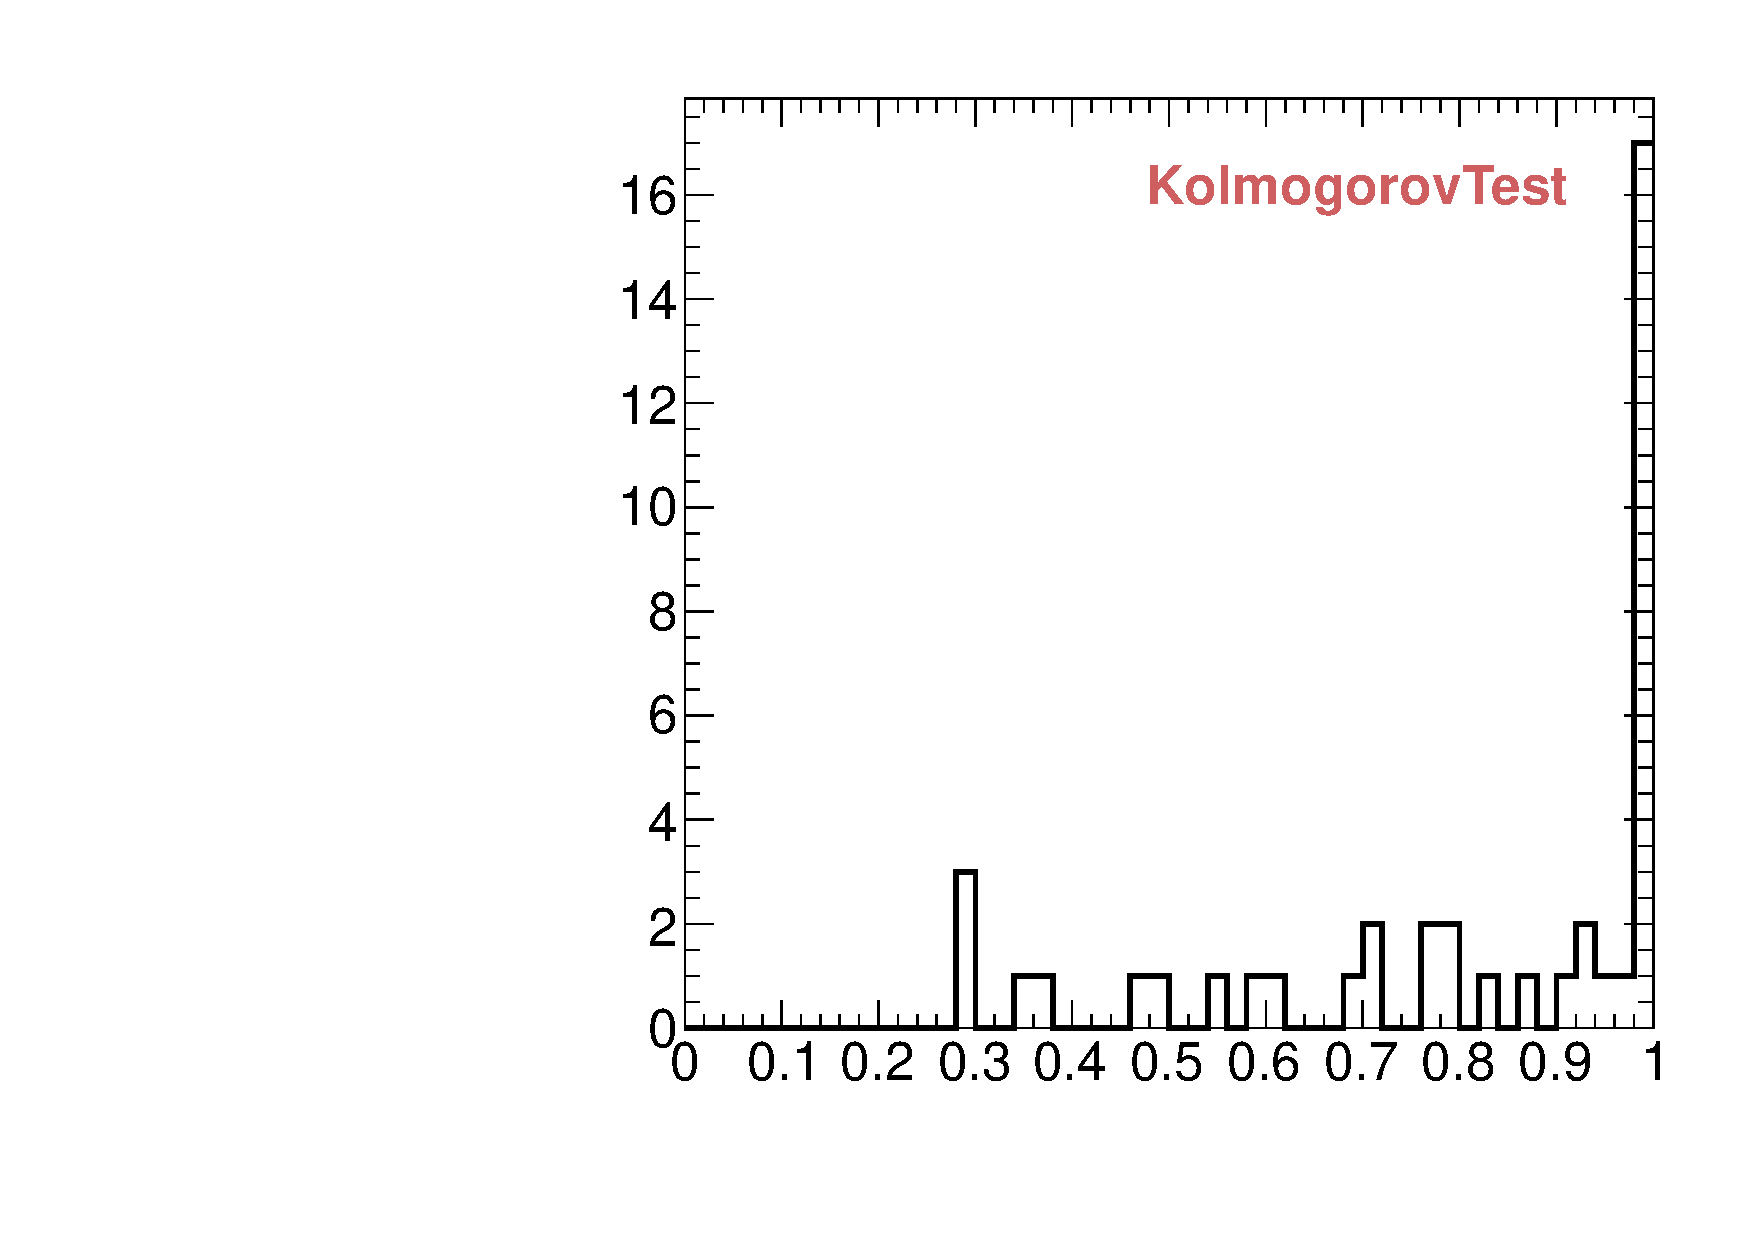
\includegraphics[width=\textwidth]{Figures/VariablesComparison/MC_endcaps_figs_3h/KS}
                \label{fig:MC_endcaps_KS_3h}
        \end{subfigure}
        \caption{Overlay of BDT training variable distributions in Signal MC for events of the three subsets in the endcap. The plot on the bottom right summarizes all KS probablities.}
        \label{fig:MC_endcaps_figs_3h}
\end{sidewaysfigure}


\begin{sidewaysfigure}
        \centering
        \begin{subfigure}[b]{0.2\textwidth}
                \centering
                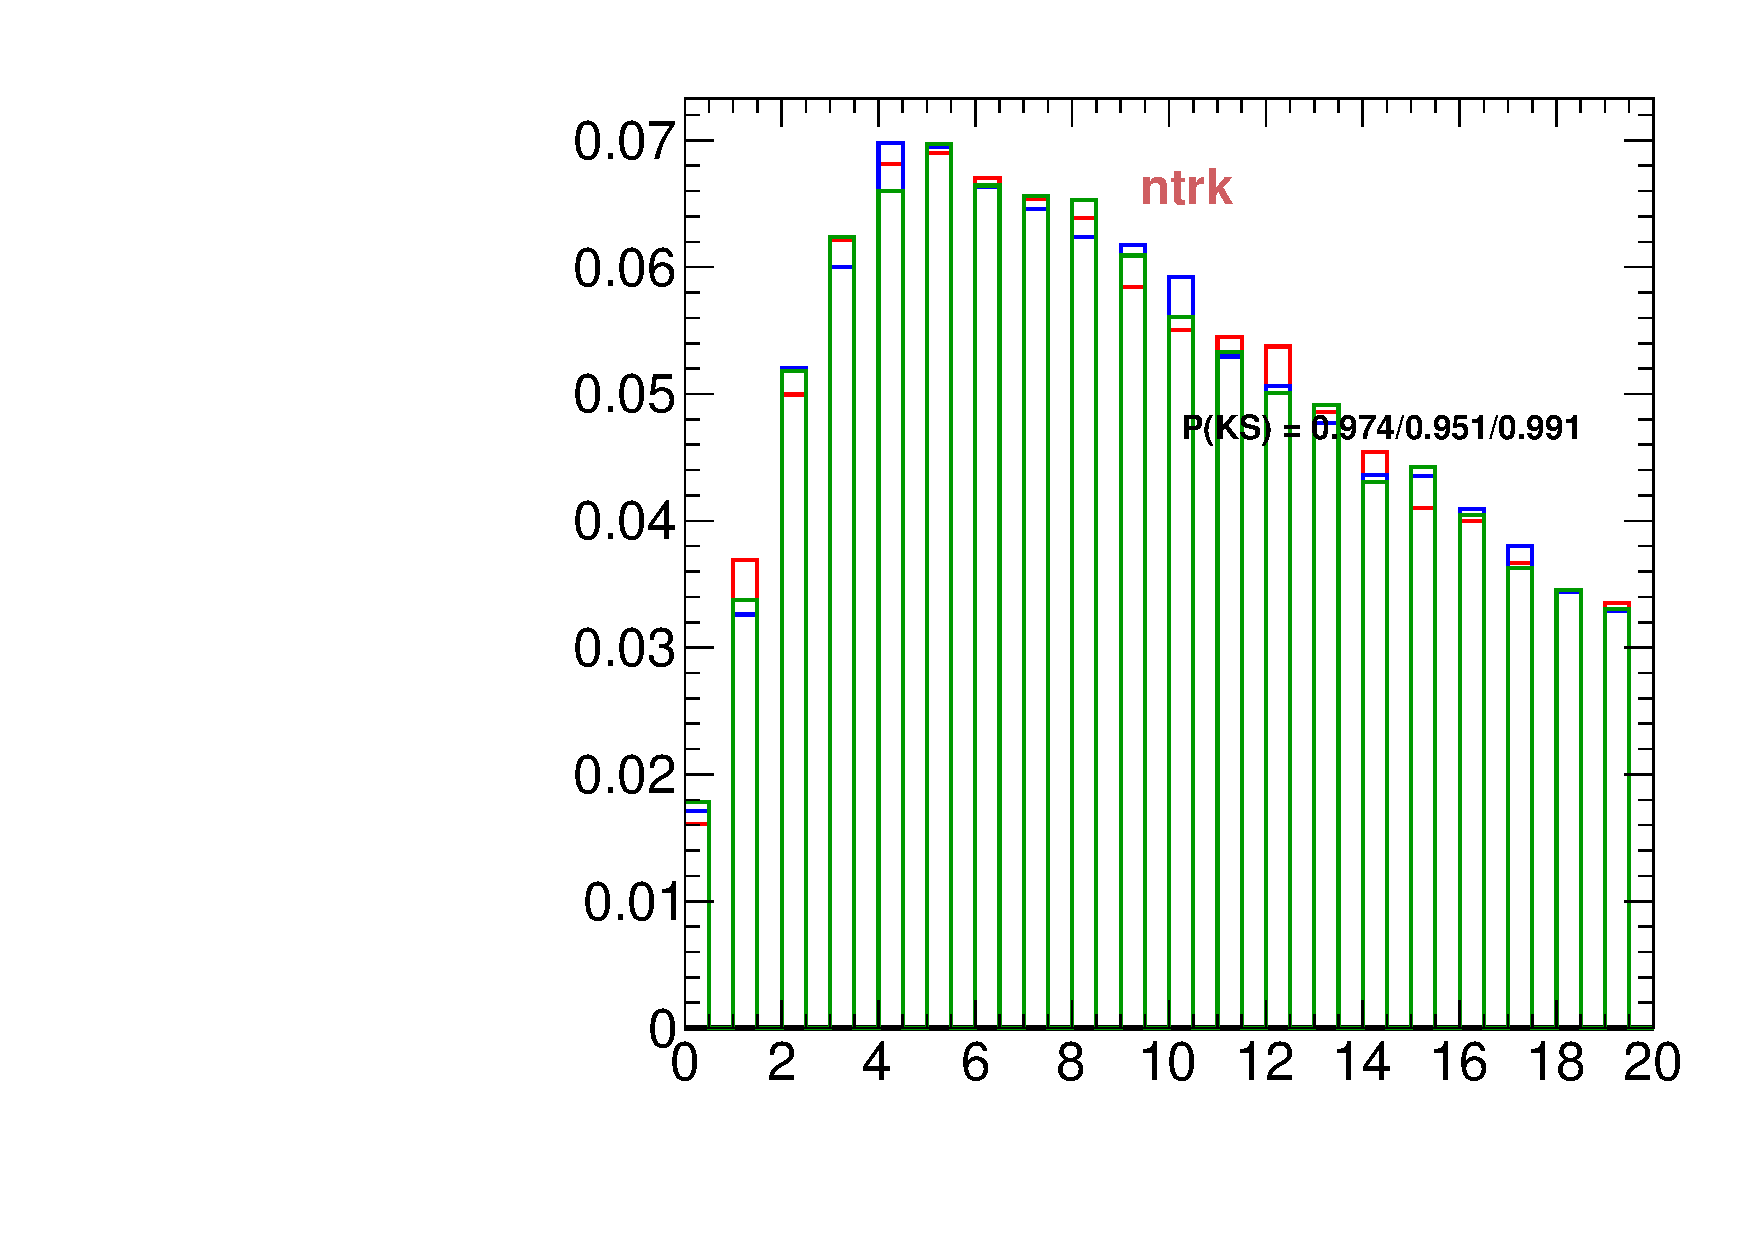
\includegraphics[width=\textwidth]{Figures/VariablesComparison/Data_barrel_figs_3h/ntrk}
                \label{fig:Data_barrel_ntrk_3h}
        \end{subfigure}
        \begin{subfigure}[b]{0.2\textwidth}
                \centering
                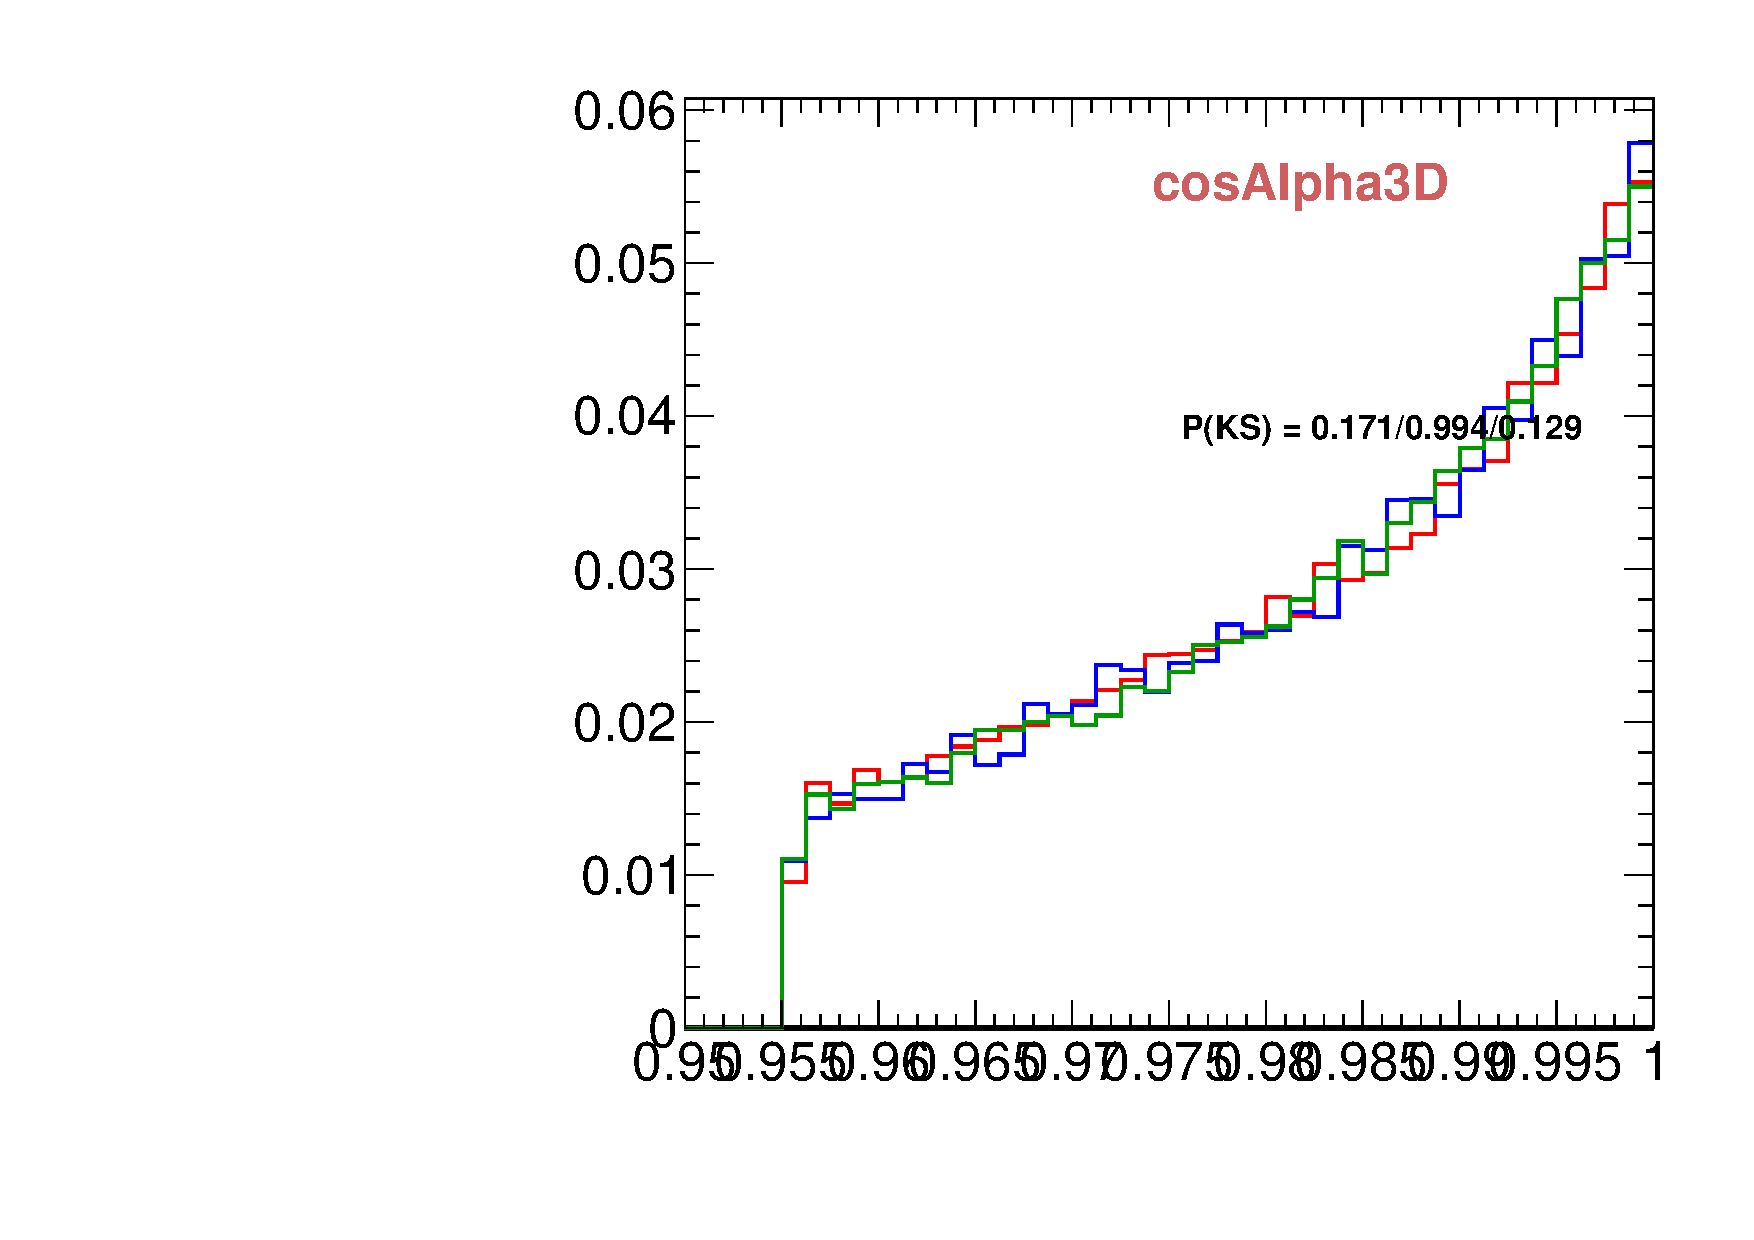
\includegraphics[width=\textwidth]{Figures/VariablesComparison/Data_barrel_figs_3h/cosAlpha3D}
                \label{fig:Data_barrel_cosAlpha3D_3h}
        \end{subfigure}
        \begin{subfigure}[b]{0.2\textwidth}
                \centering
                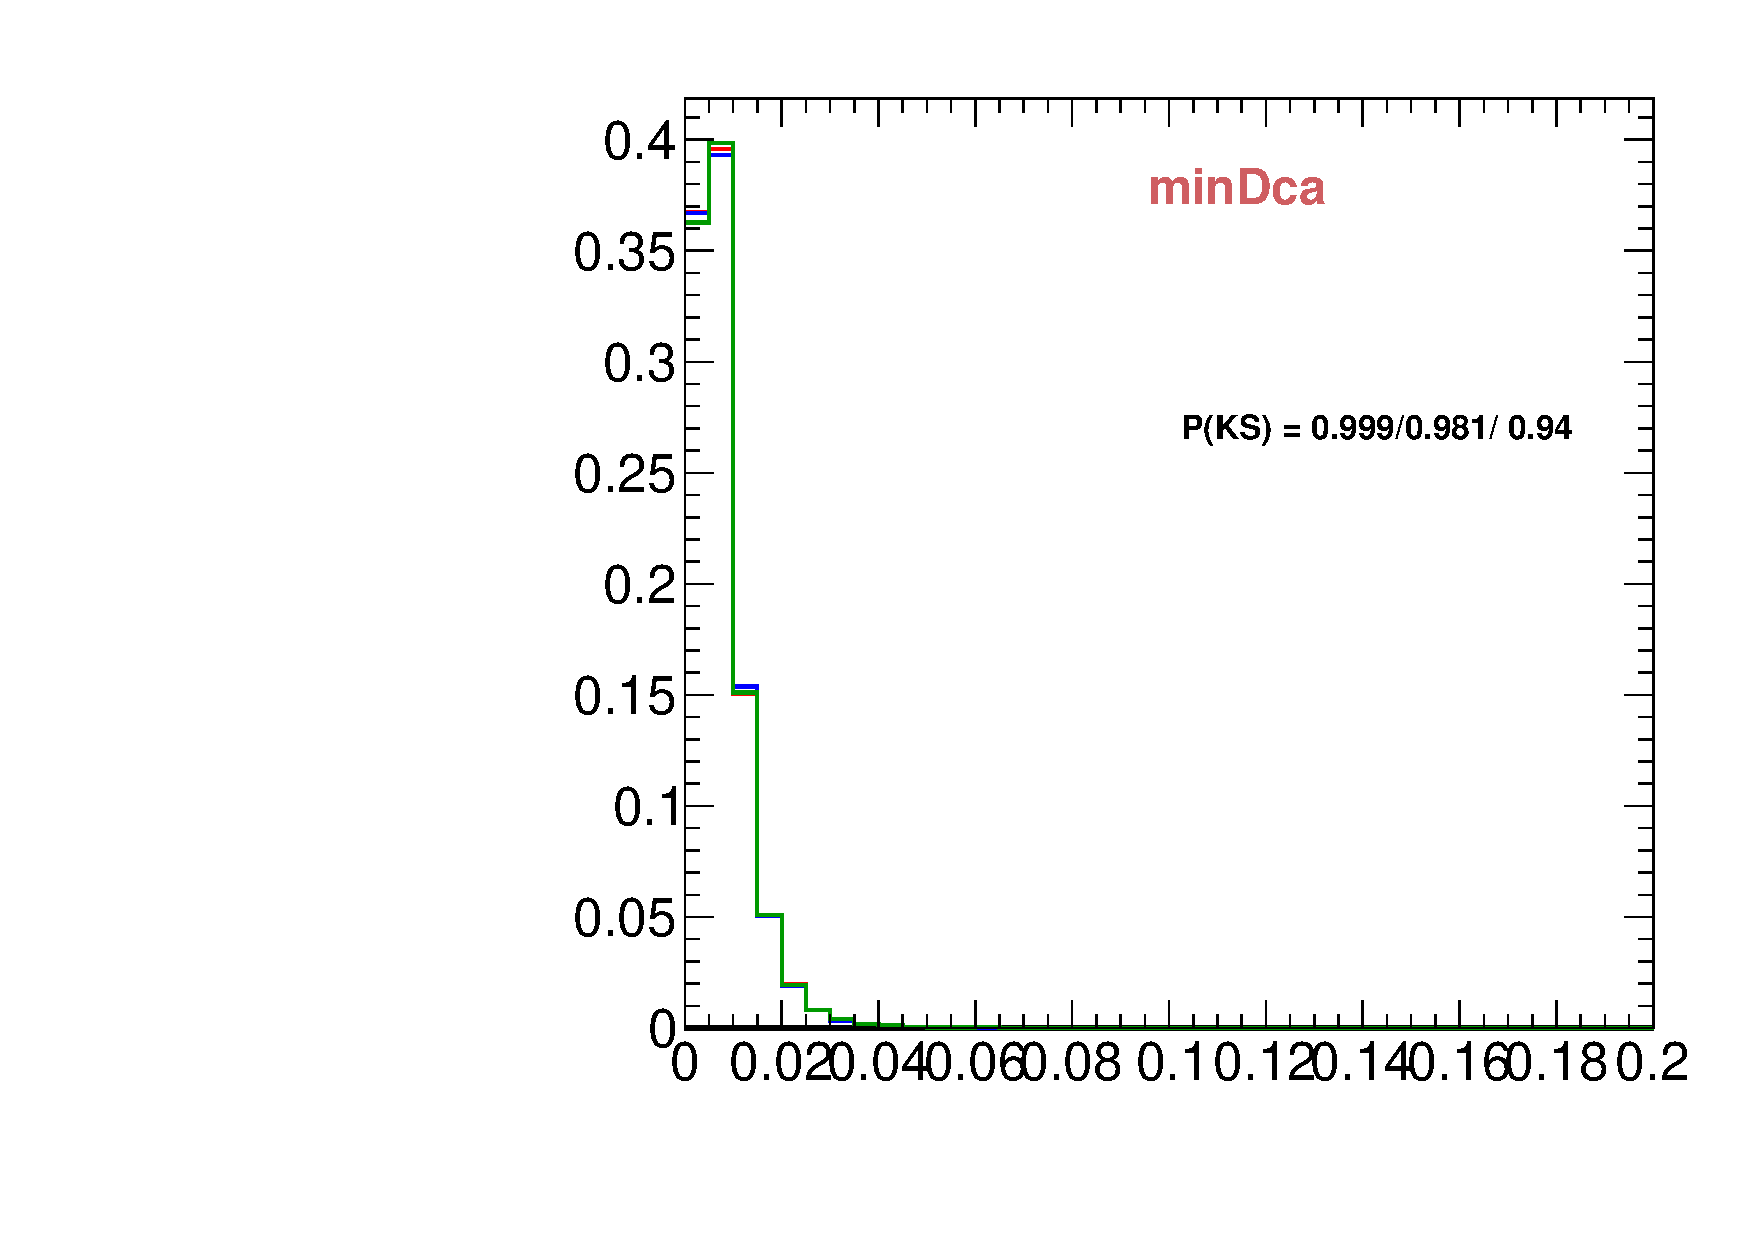
\includegraphics[width=\textwidth]{Figures/VariablesComparison/Data_barrel_figs_3h/minDca}
                \label{fig:Data_barrel_minDca_3h}
        \end{subfigure}
        \begin{subfigure}[b]{0.2\textwidth}
                \centering
                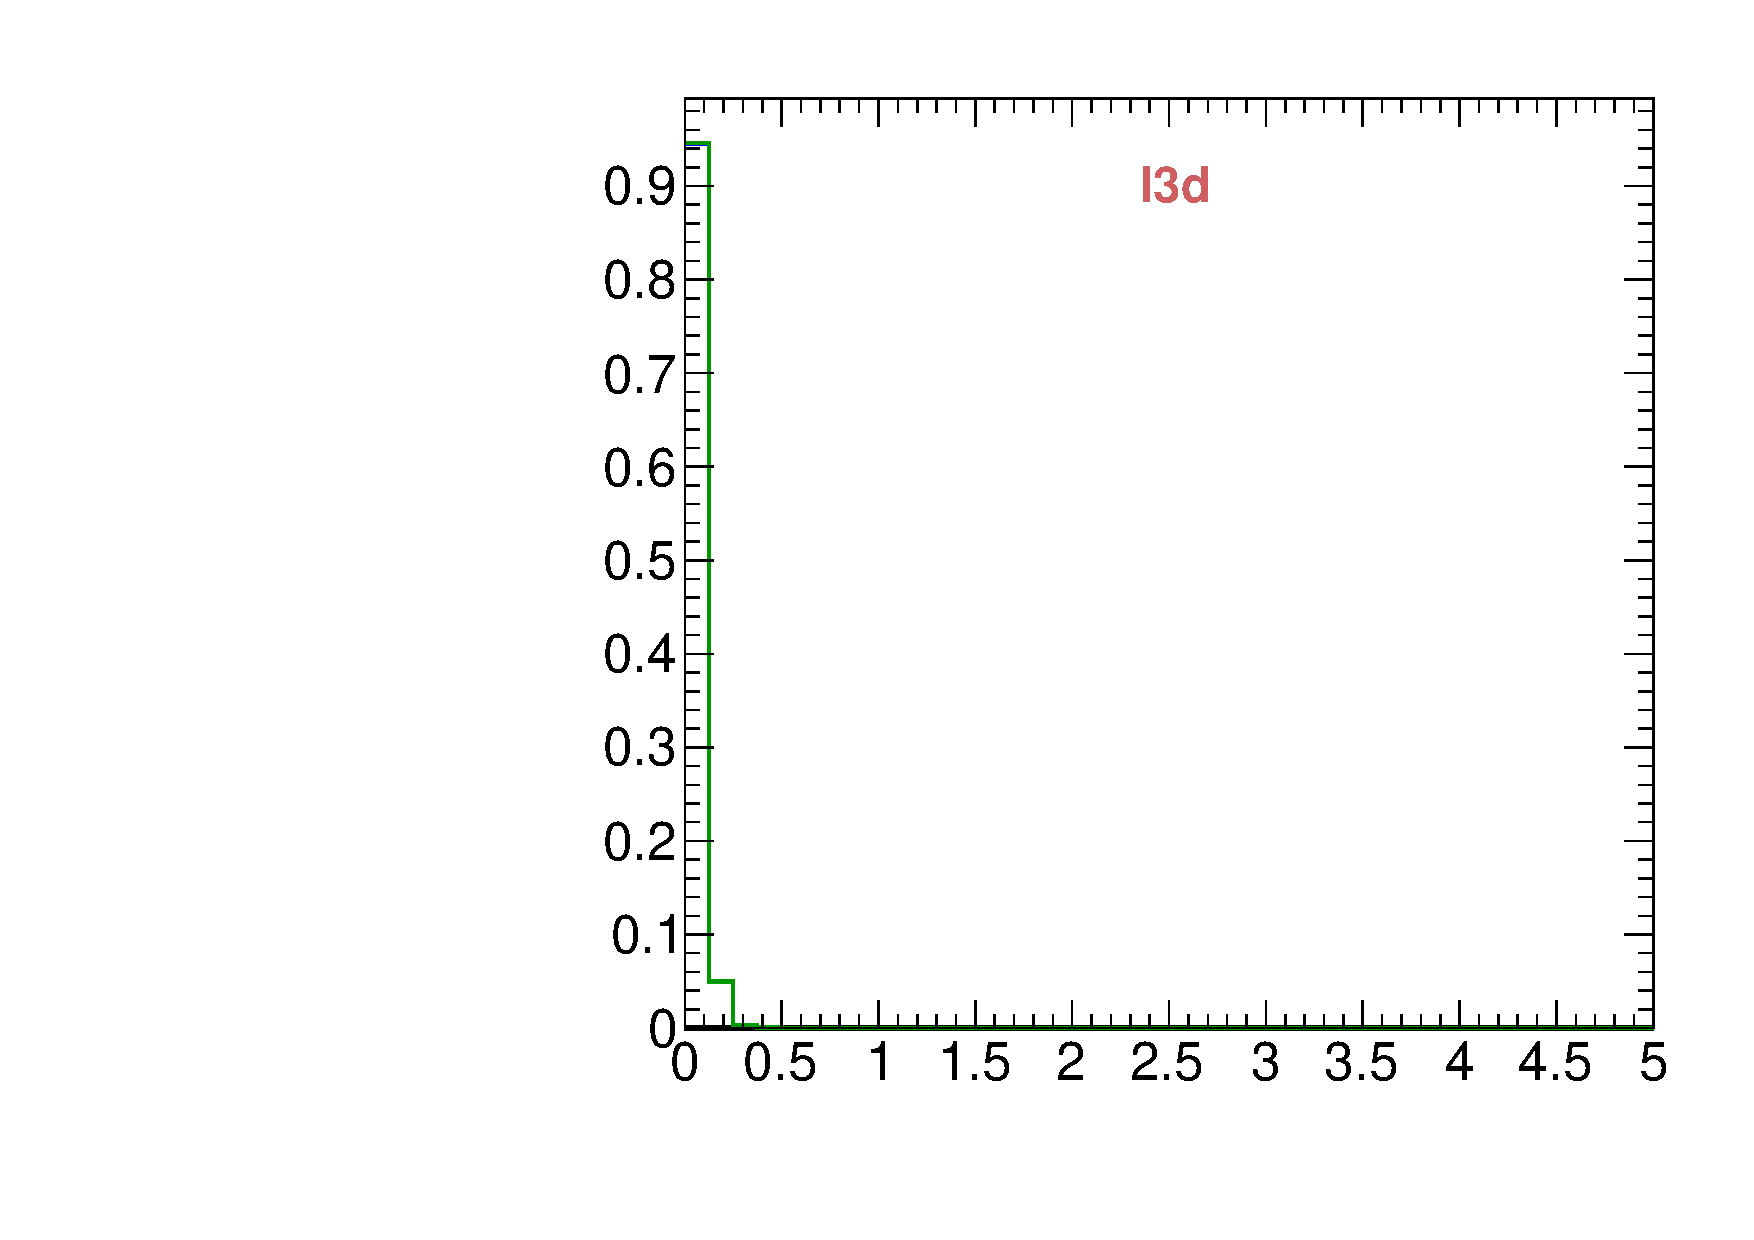
\includegraphics[width=\textwidth]{Figures/VariablesComparison/Data_barrel_figs_3h/l3d}
                \label{fig:Data_barrel_l3d_3h}
        \end{subfigure}
        \begin{subfigure}[b]{0.2\textwidth}
                \centering
                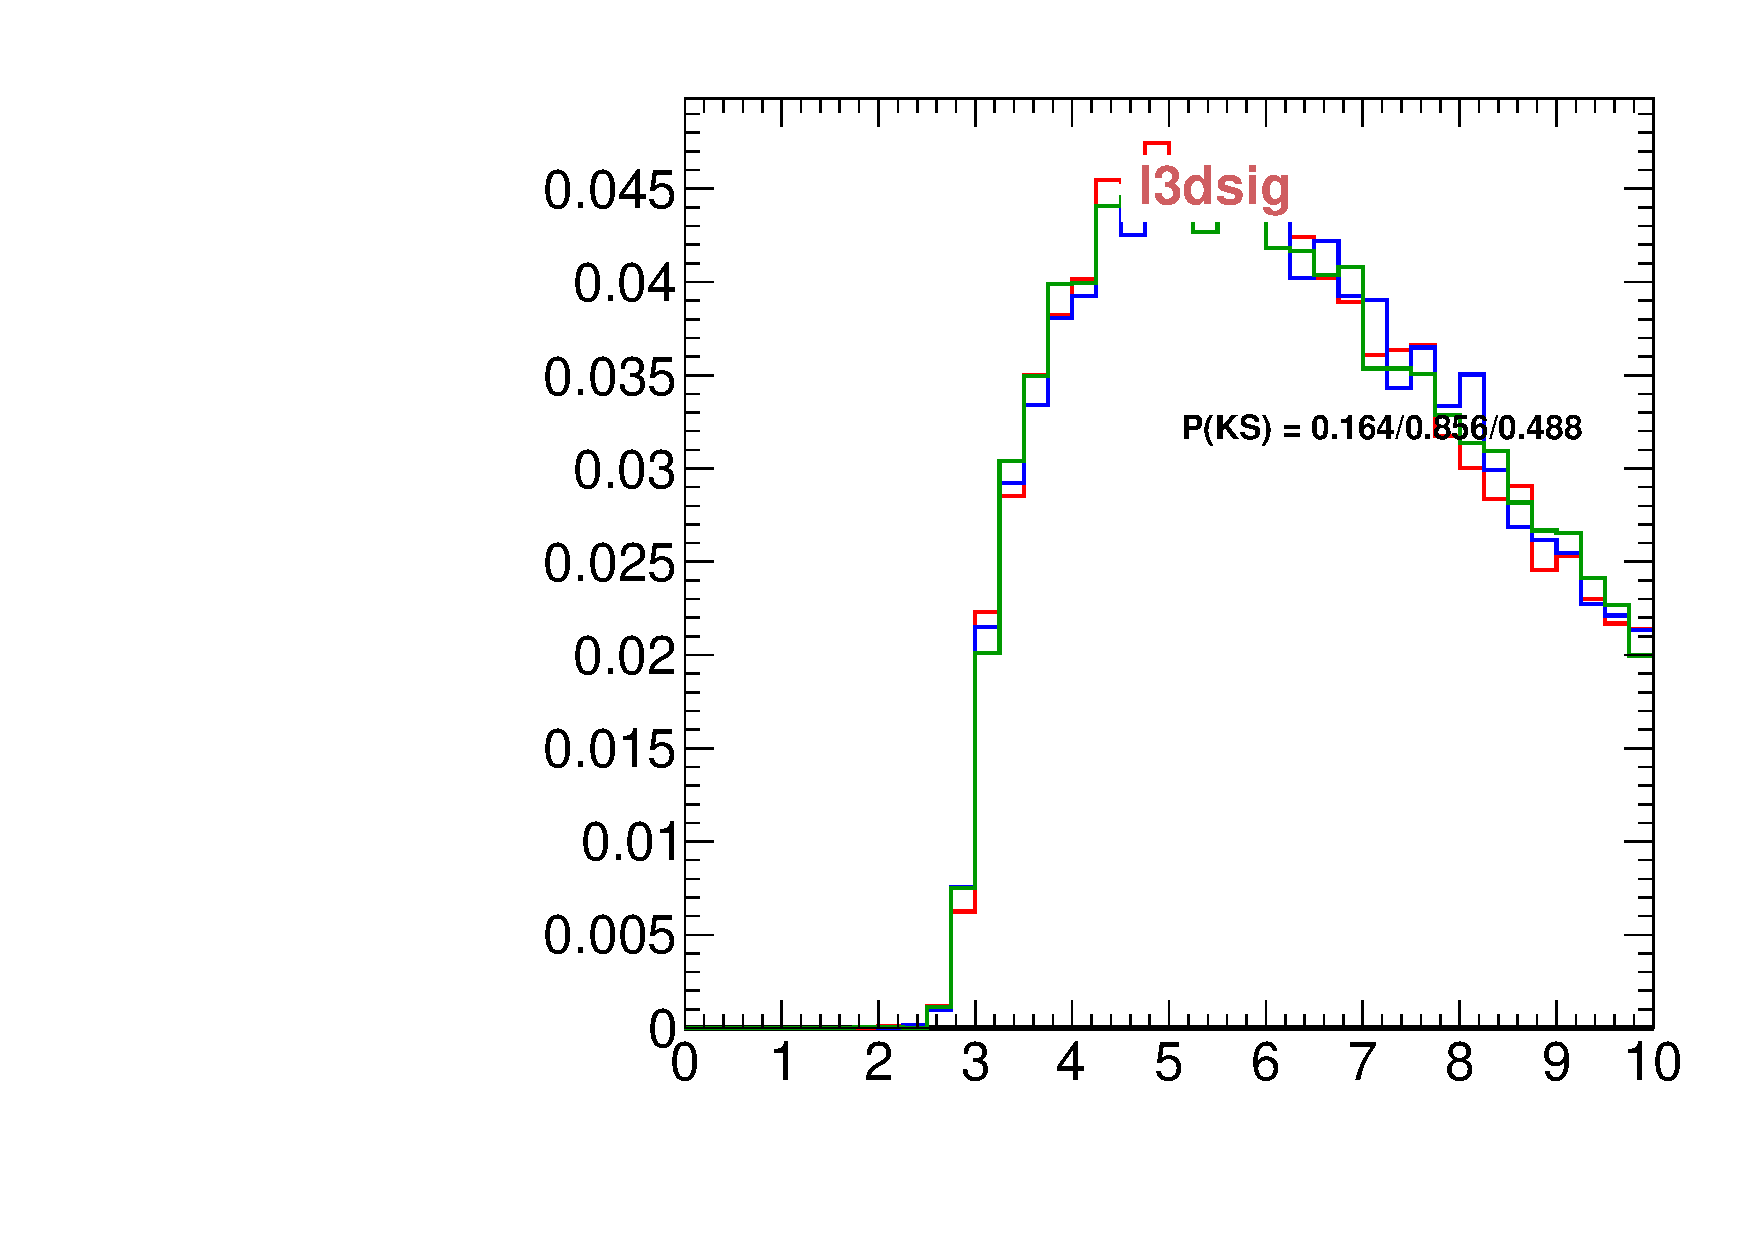
\includegraphics[width=\textwidth]{Figures/VariablesComparison/Data_barrel_figs_3h/l3dsig}
                \label{fig:Data_barrel_l3dsig_3h}
        \end{subfigure}
        \begin{subfigure}[b]{0.2\textwidth}
                \centering
                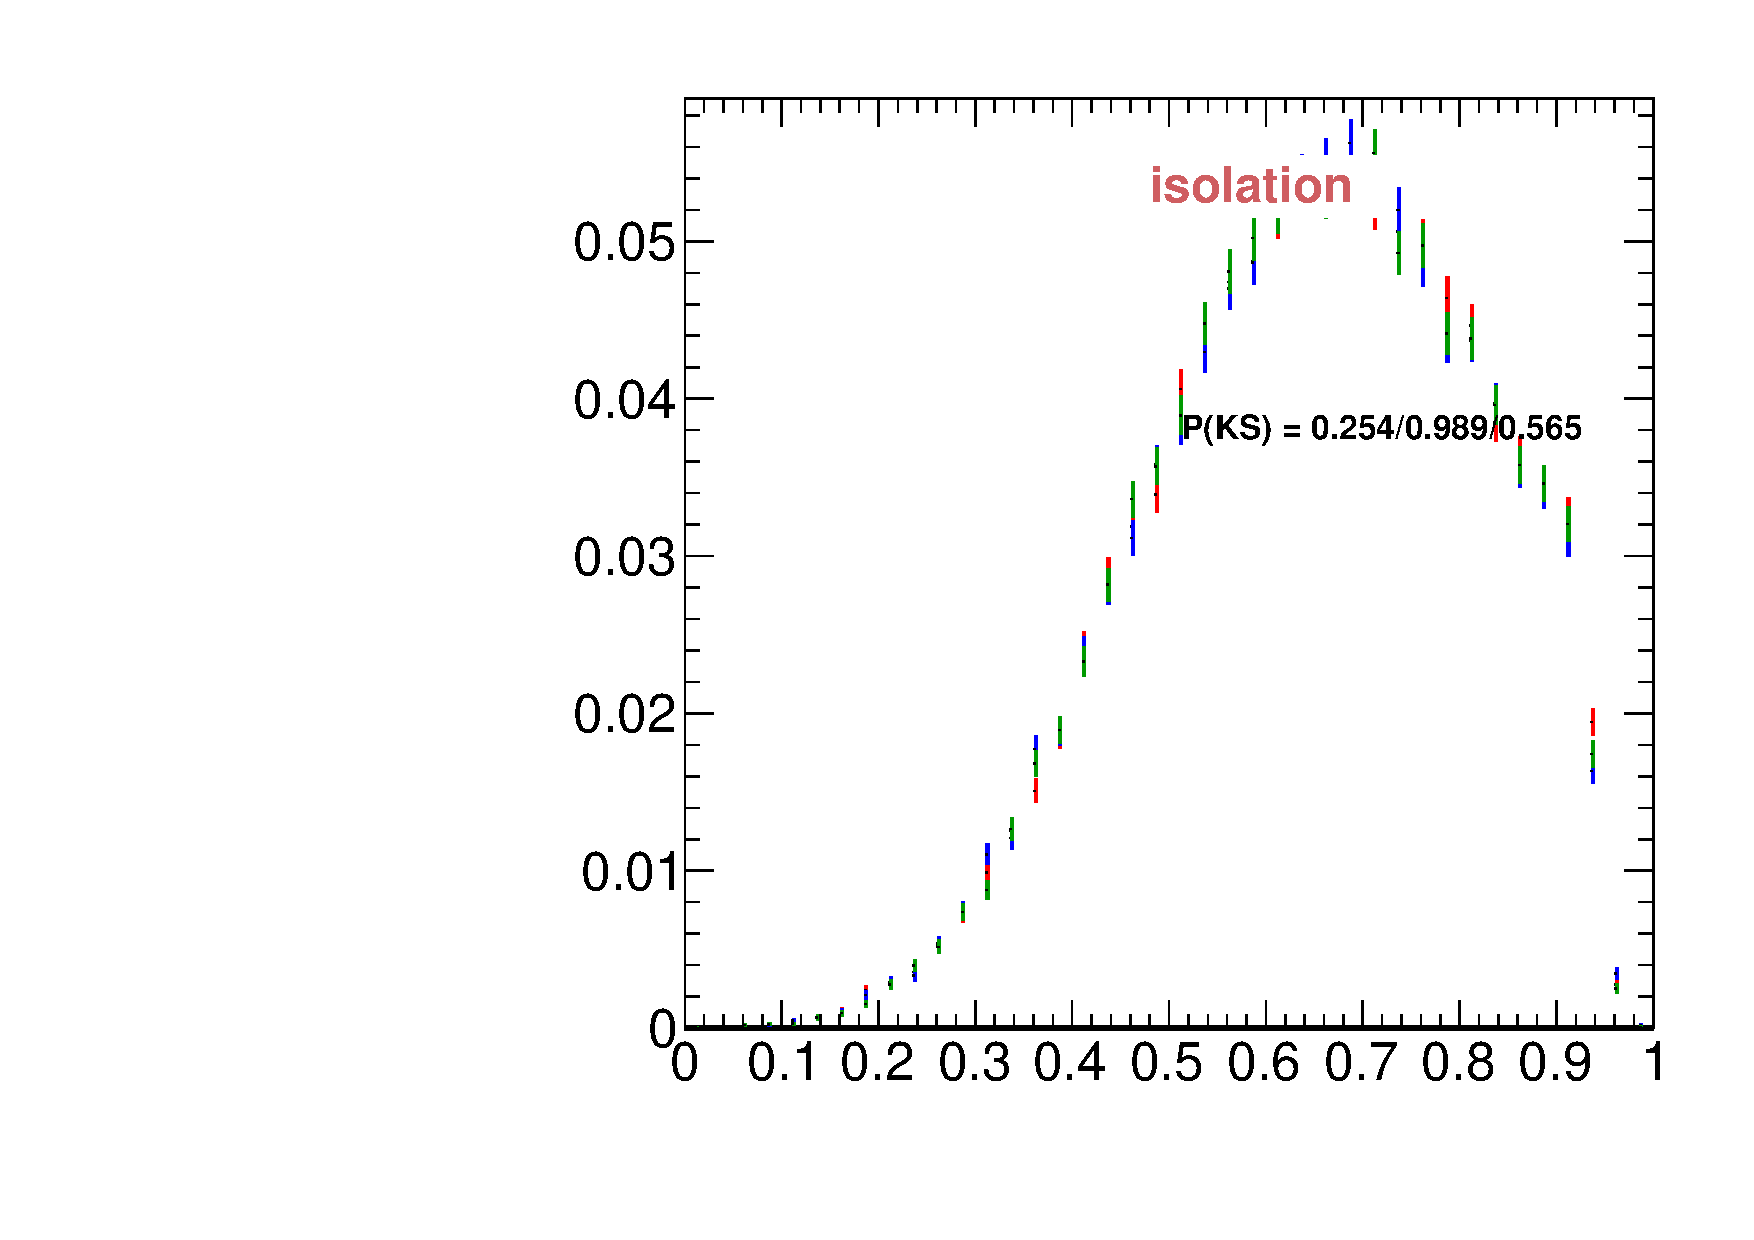
\includegraphics[width=\textwidth]{Figures/VariablesComparison/Data_barrel_figs_3h/isolation}
                \label{fig:Data_barrel_isolation_3h}
        \end{subfigure}
        \begin{subfigure}[b]{0.2\textwidth}
                \centering
                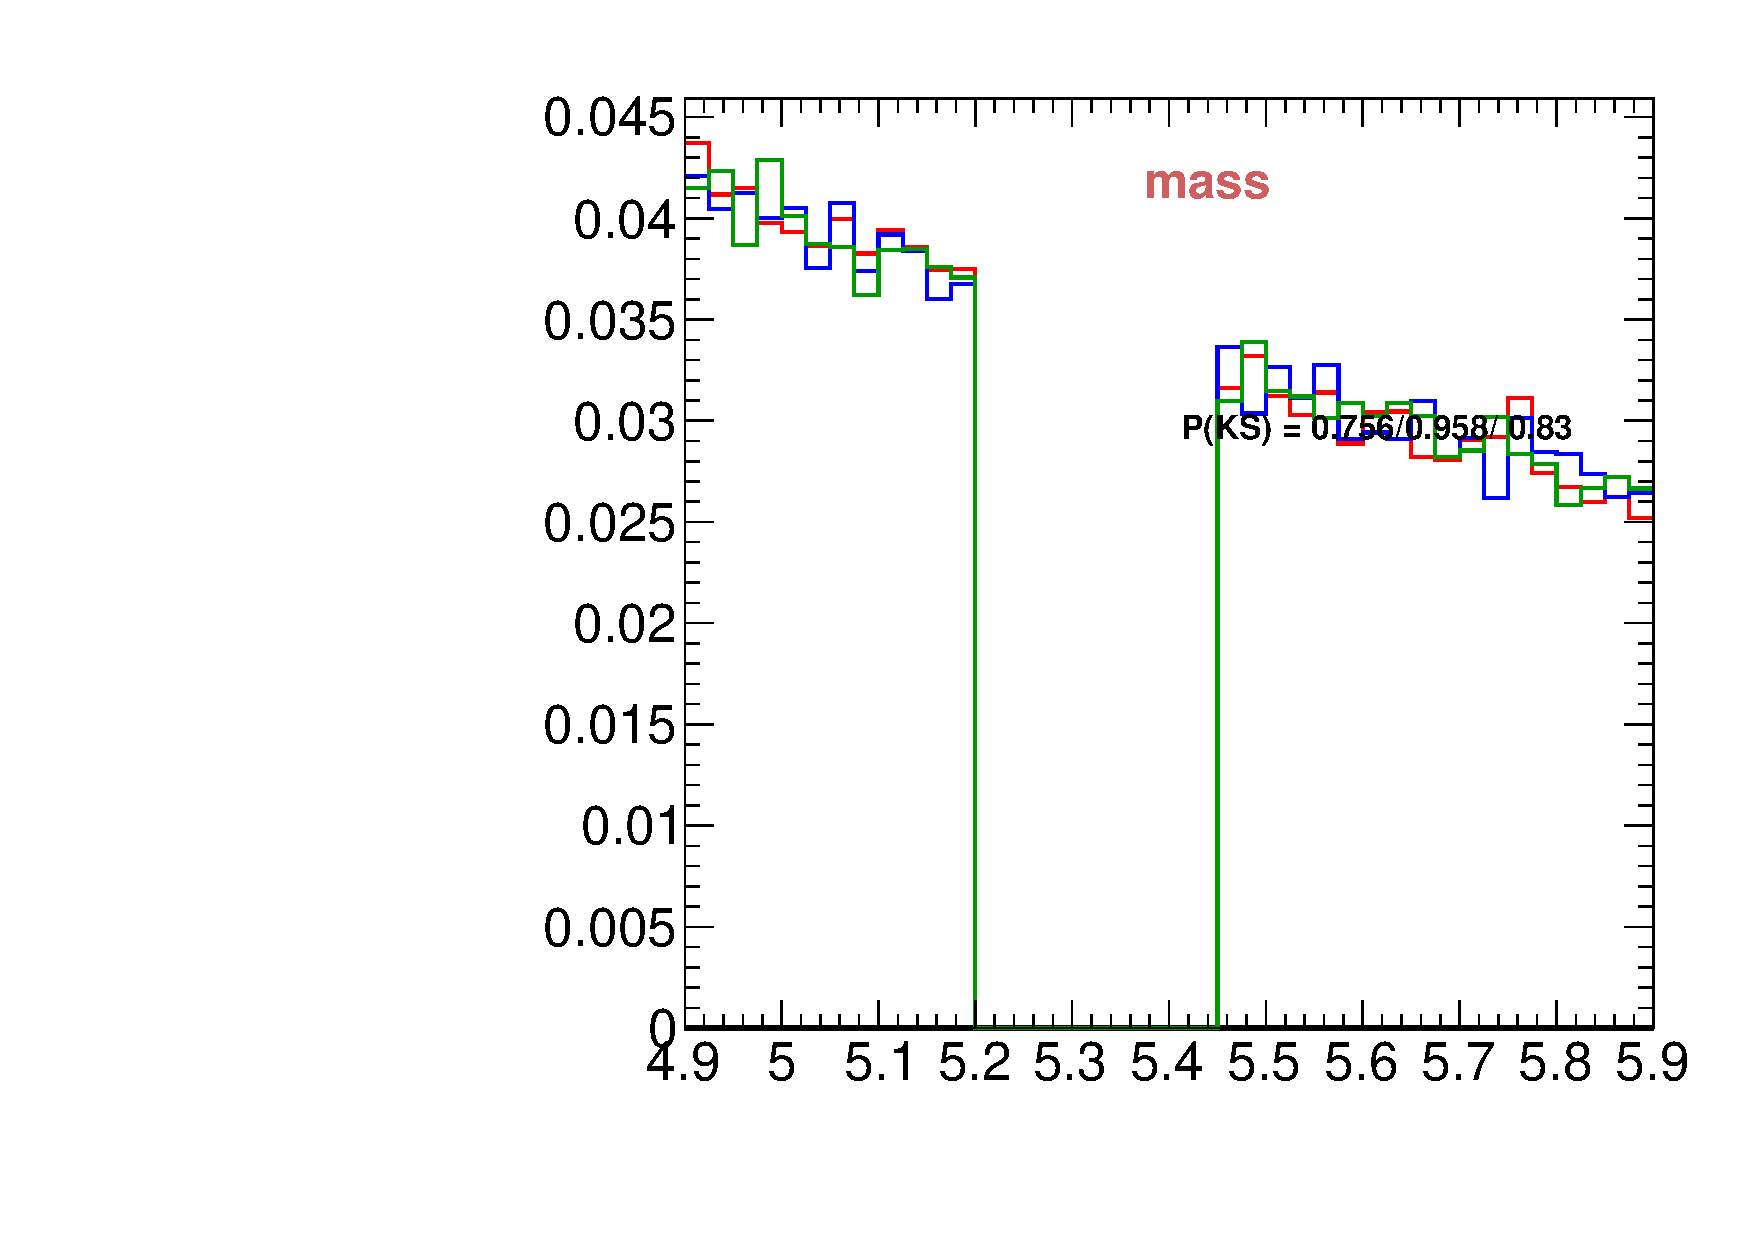
\includegraphics[width=\textwidth]{Figures/VariablesComparison/Data_barrel_figs_3h/mass}
                \label{fig:Data_barrel_mass_3h}
        \end{subfigure}
        \begin{subfigure}[b]{0.2\textwidth}
                \centering
                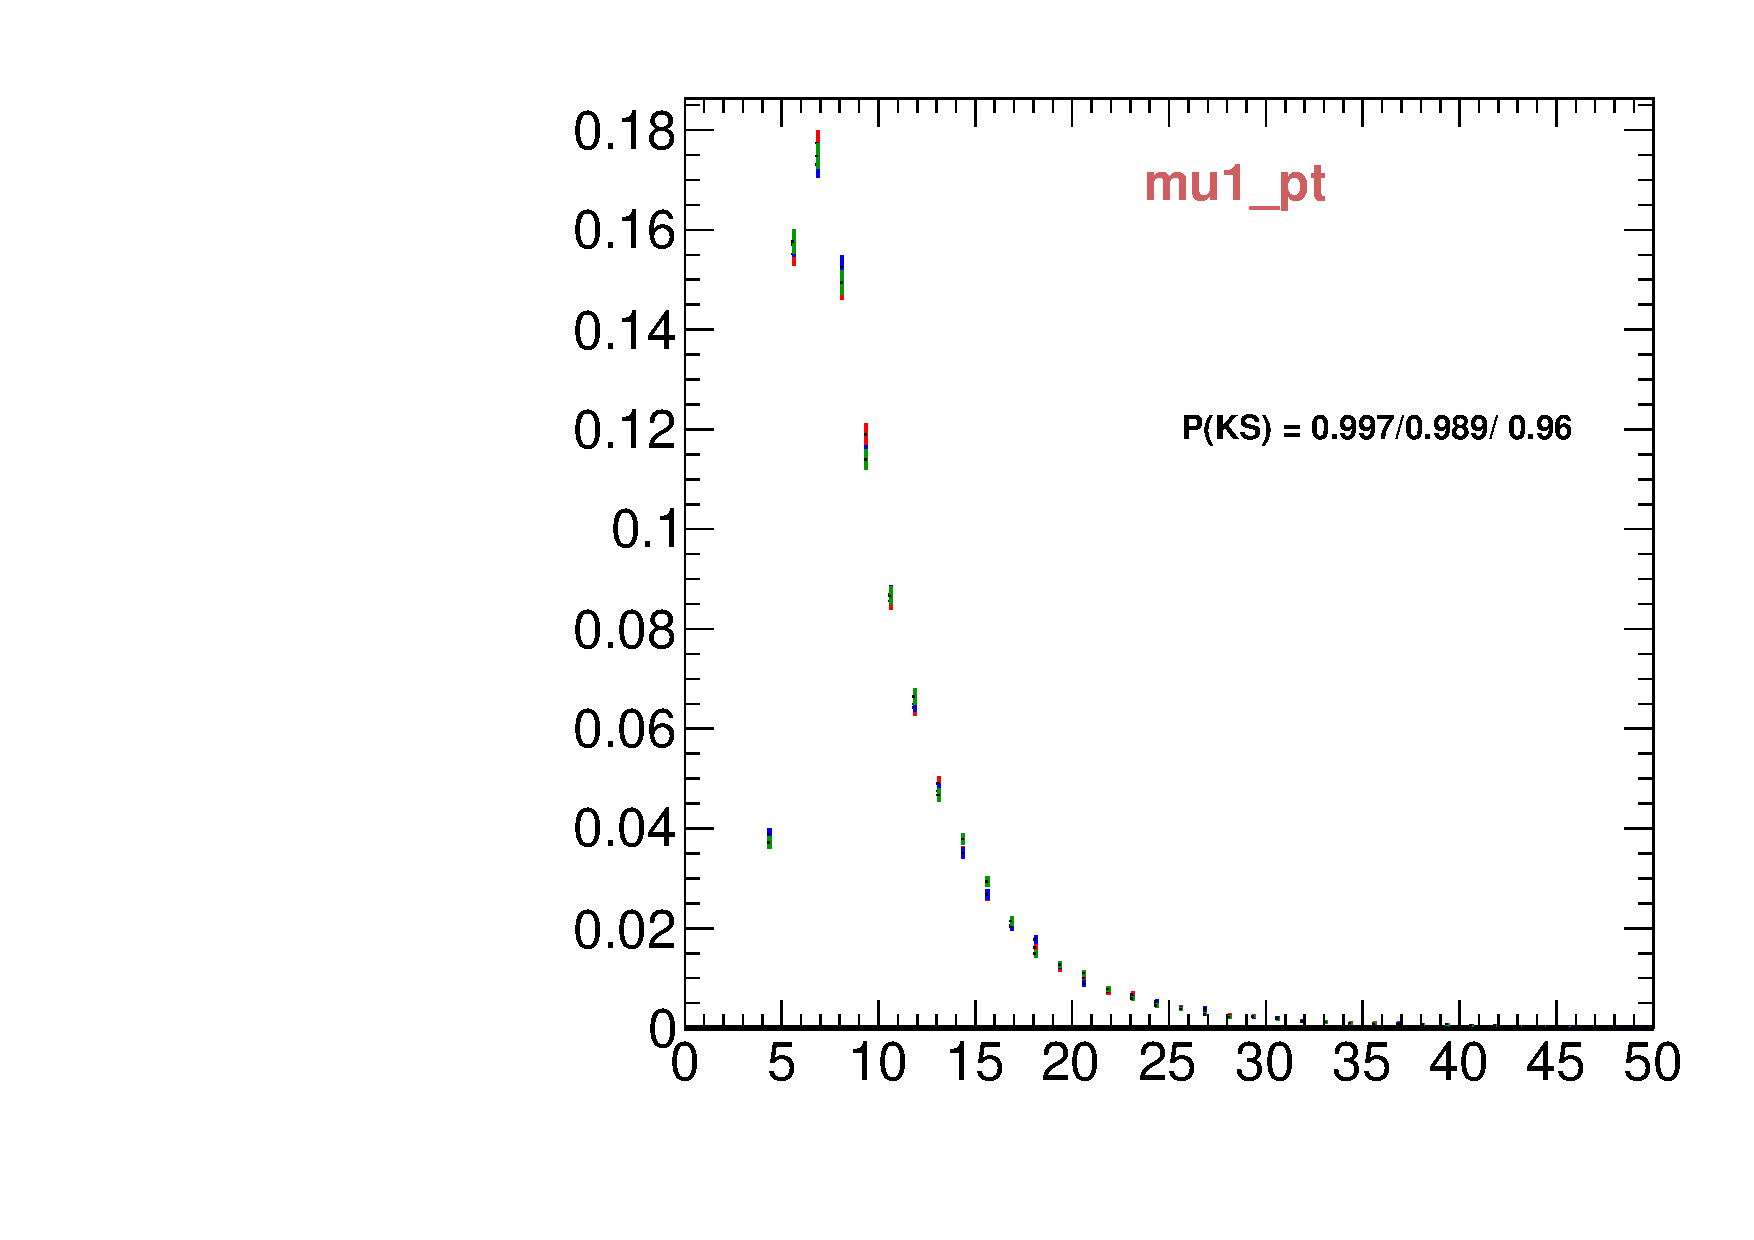
\includegraphics[width=\textwidth]{Figures/VariablesComparison/Data_barrel_figs_3h/mu1_pt}
                \label{fig:Data_barrel_mu1_pt_3h}
        \end{subfigure}
        \begin{subfigure}[b]{0.2\textwidth}
                \centering
                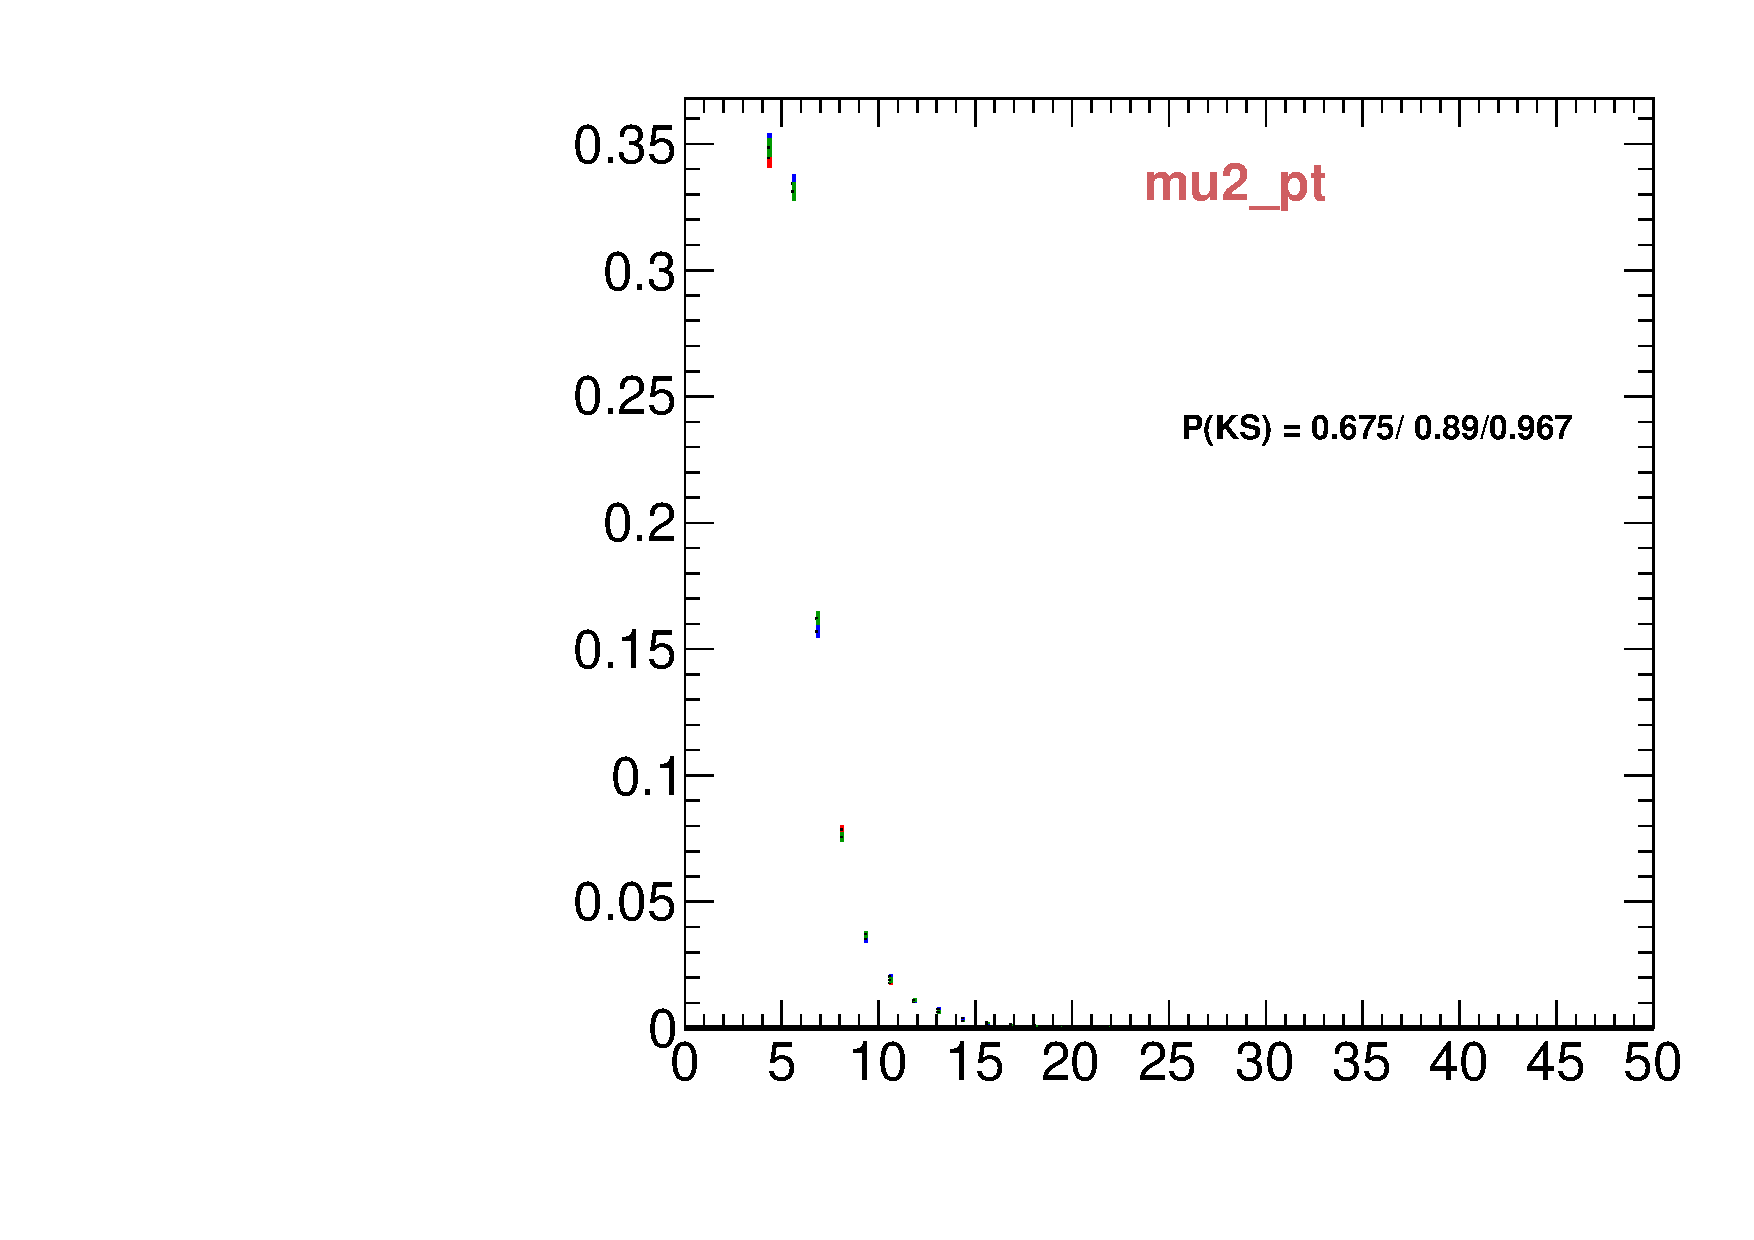
\includegraphics[width=\textwidth]{Figures/VariablesComparison/Data_barrel_figs_3h/mu2_pt}
                \label{fig:Data_barrel_mu2_pt_3h}
        \end{subfigure}
        \begin{subfigure}[b]{0.2\textwidth}
                \centering
                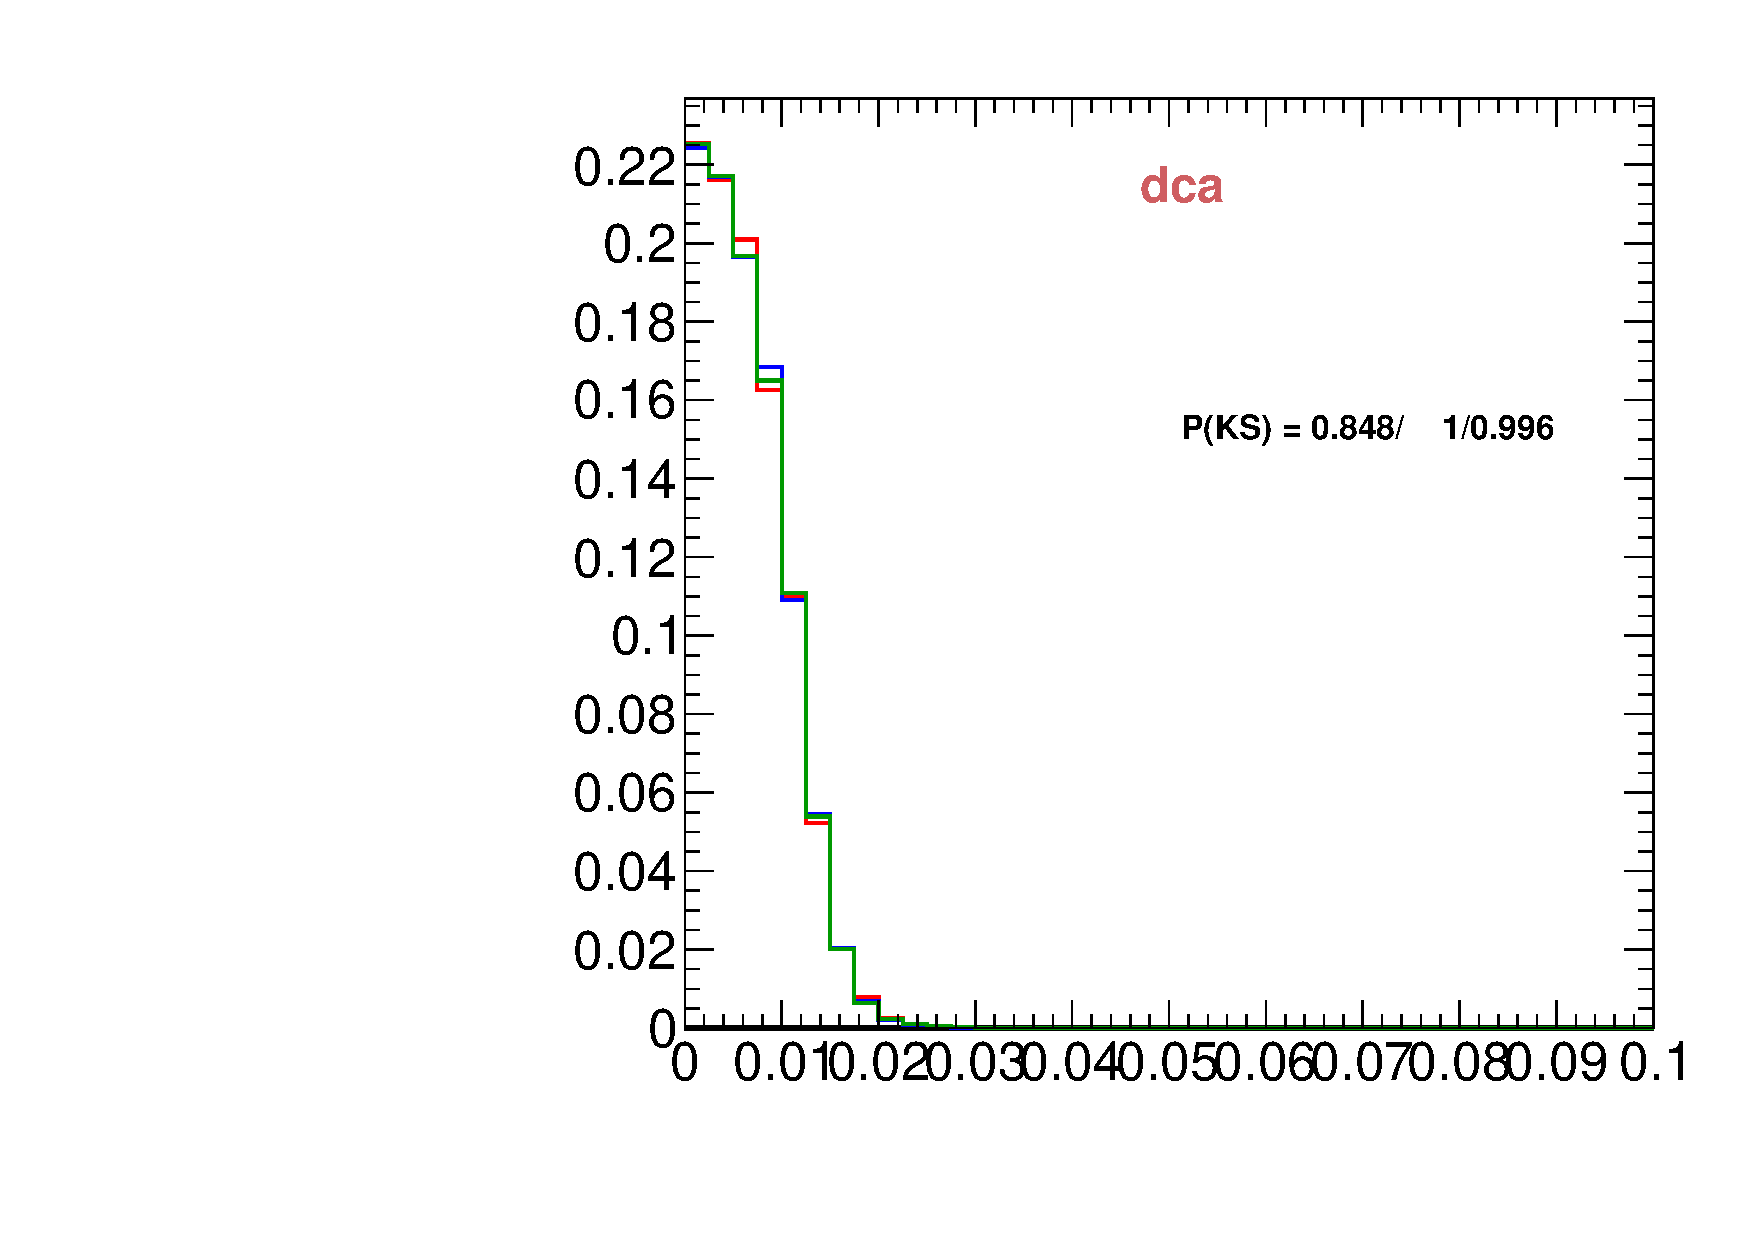
\includegraphics[width=\textwidth]{Figures/VariablesComparison/Data_barrel_figs_3h/dca}
                \label{fig:Data_barrel_dca_3h}
        \end{subfigure}
        \begin{subfigure}[b]{0.2\textwidth}
                \centering
                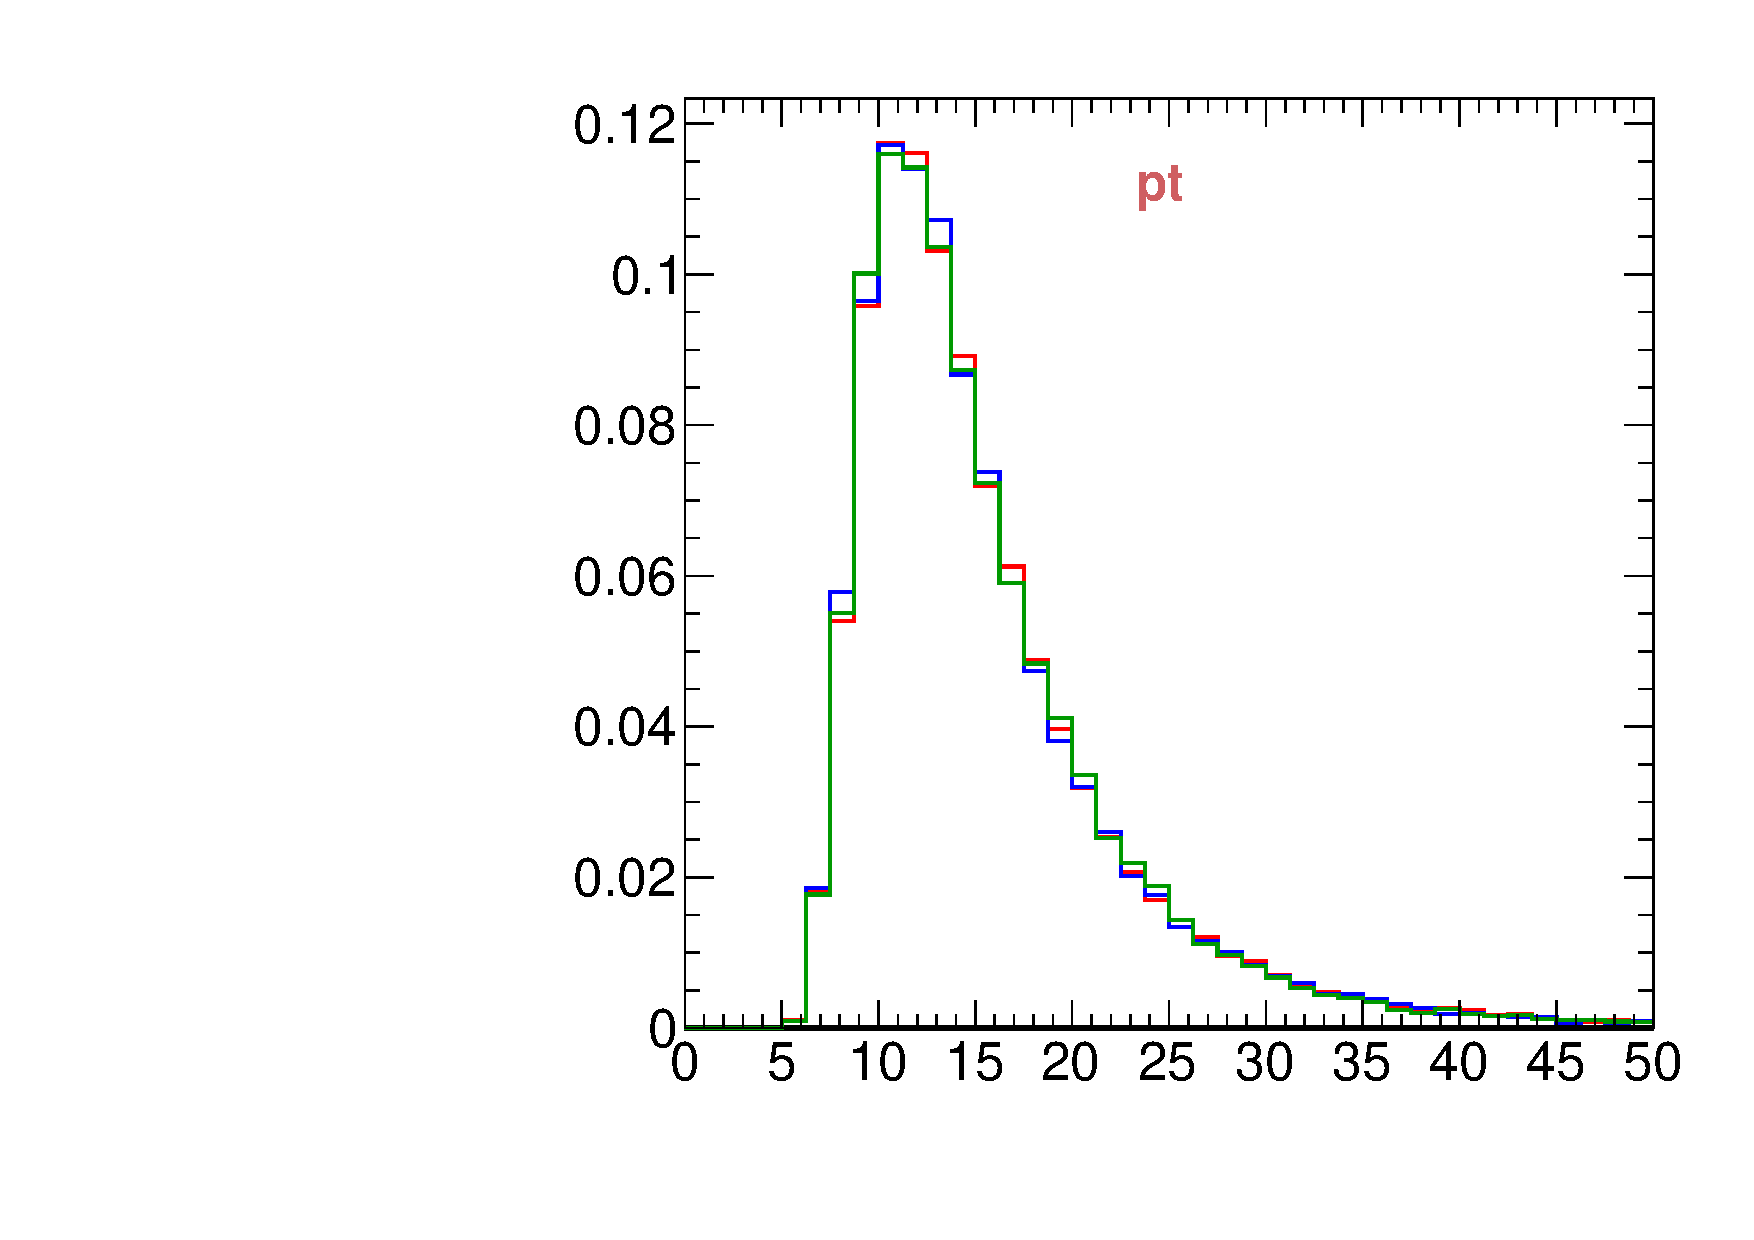
\includegraphics[width=\textwidth]{Figures/VariablesComparison/Data_barrel_figs_3h/pt}
                \label{fig:Data_barrel_pt_3h}
        \end{subfigure}
        \begin{subfigure}[b]{0.2\textwidth}
                \centering
                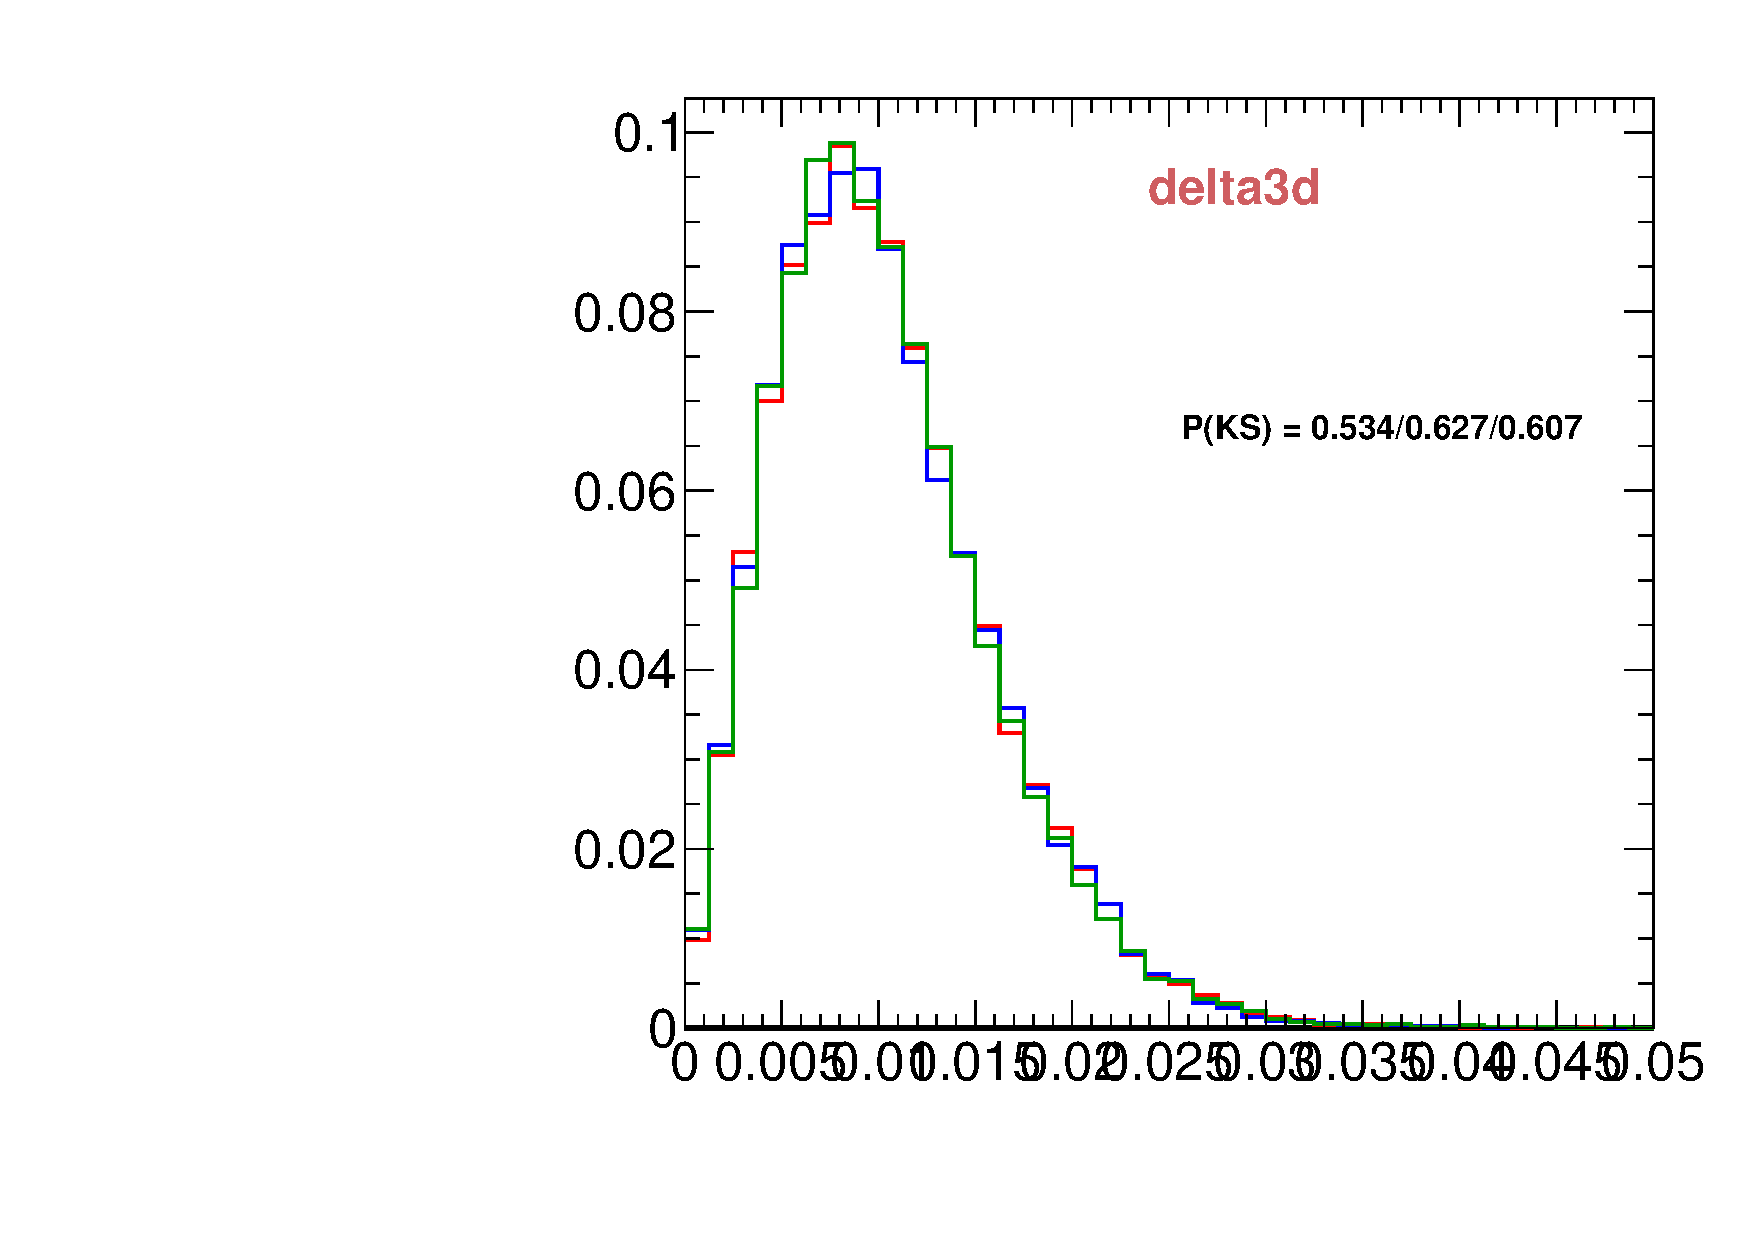
\includegraphics[width=\textwidth]{Figures/VariablesComparison/Data_barrel_figs_3h/delta3d}
                \label{fig:Data_barrel_delta3d_3h}
        \end{subfigure}
        \begin{subfigure}[b]{0.2\textwidth}
                \centering
                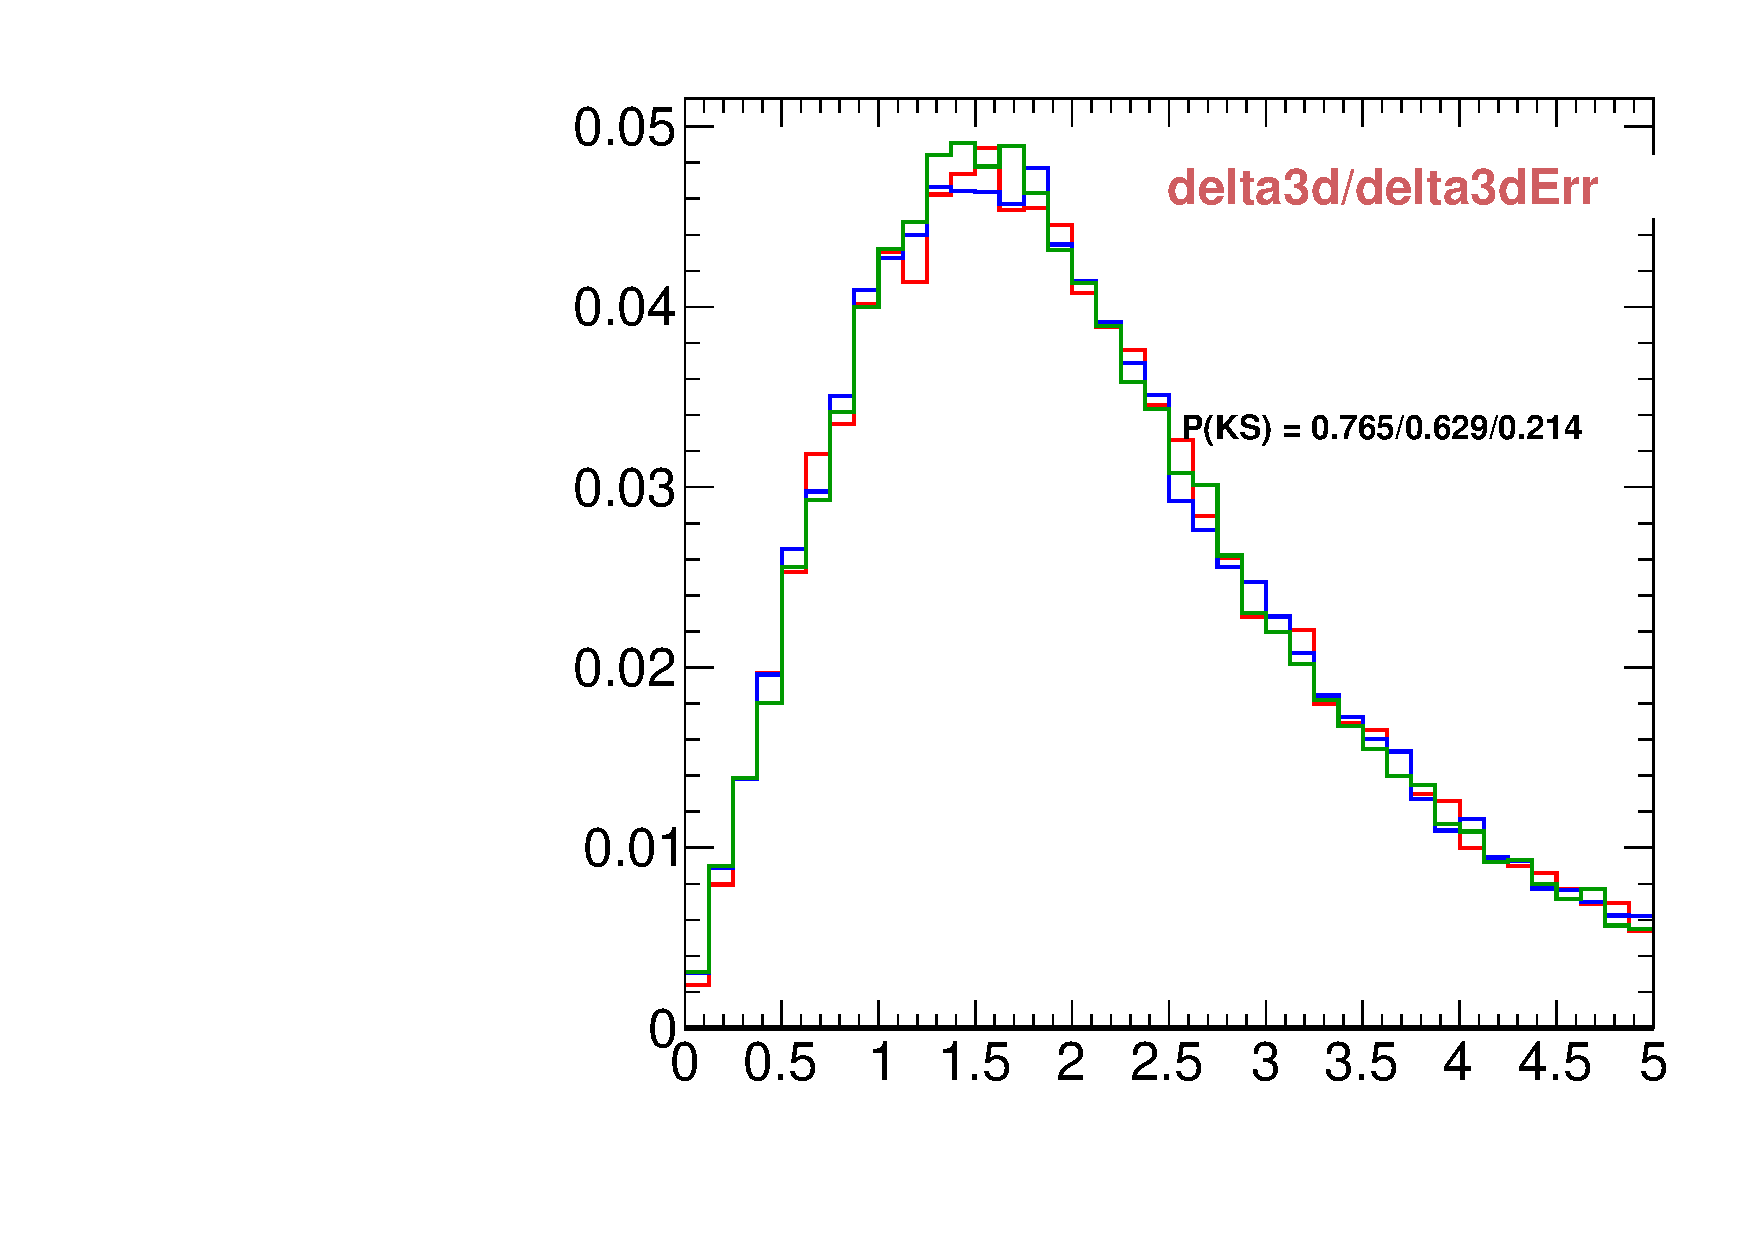
\includegraphics[width=\textwidth]{Figures/VariablesComparison/Data_barrel_figs_3h/delta3dErr}
                \label{fig:Data_barrel_delta3d/delta3dErr_3h}
        \end{subfigure}
        \begin{subfigure}[b]{0.2\textwidth}
                \centering
                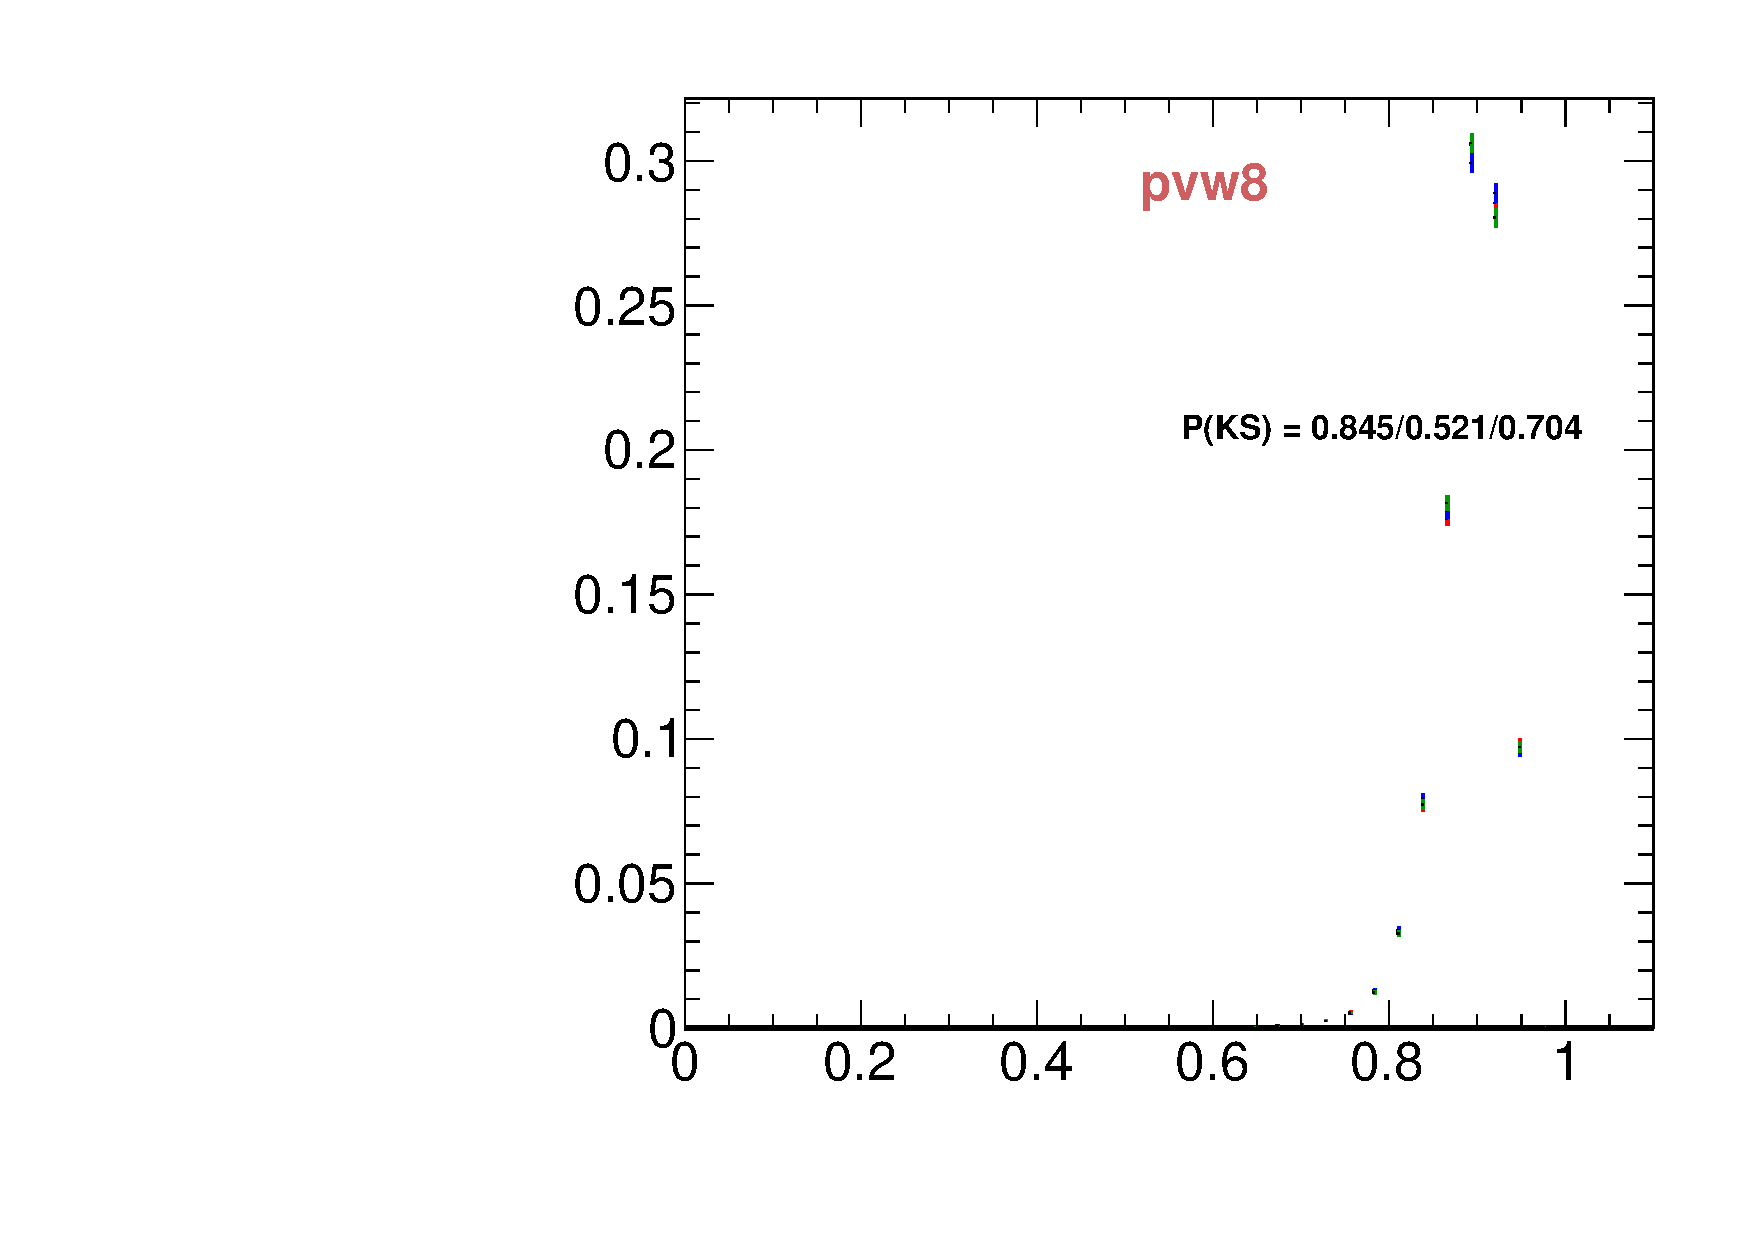
\includegraphics[width=\textwidth]{Figures/VariablesComparison/Data_barrel_figs_3h/pvw8}
                \label{fig:Data_barrel_pvw8_3h}
        \end{subfigure}
        \begin{subfigure}[b]{0.2\textwidth}
                \centering
                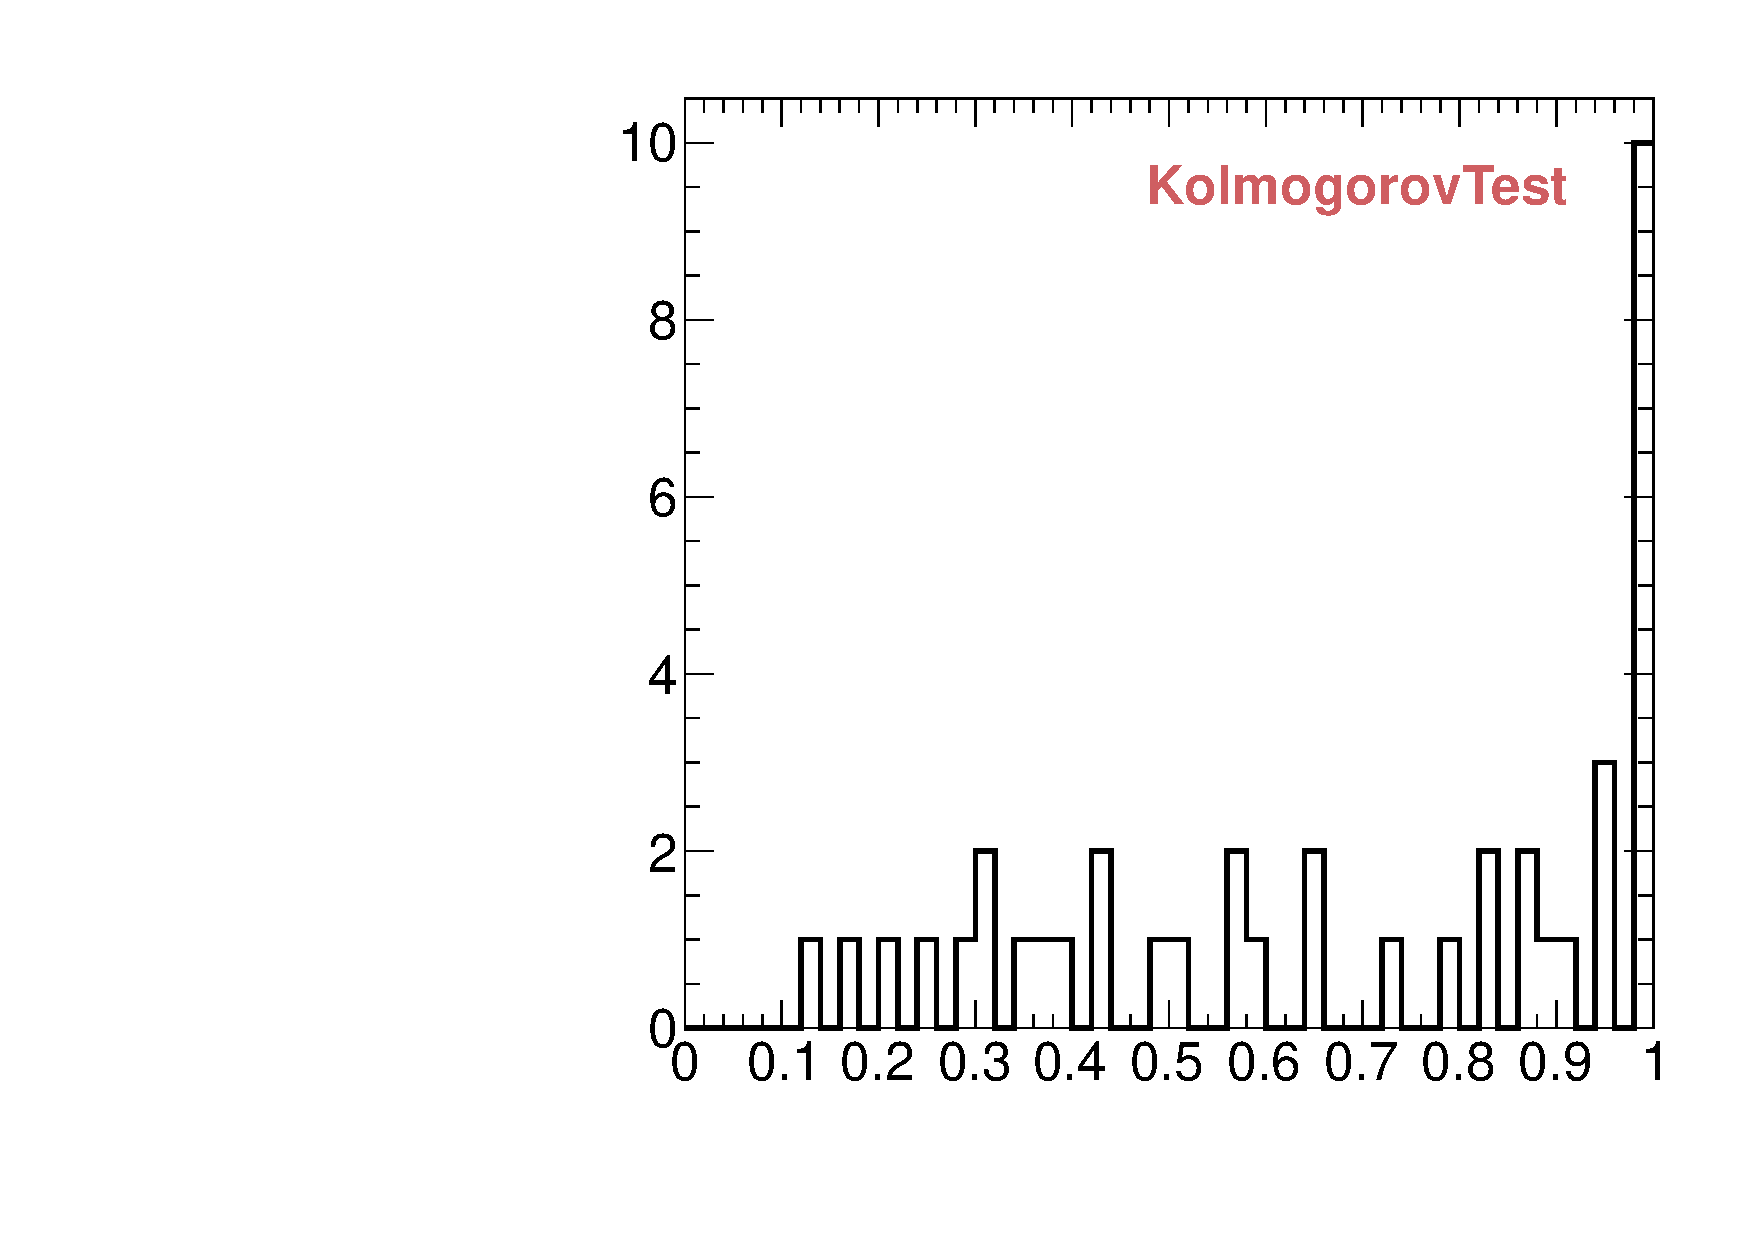
\includegraphics[width=\textwidth]{Figures/VariablesComparison/Data_barrel_figs_3h/KS}
                \label{fig:Data_barrel_KS_3h}
        \end{subfigure}
        \caption{Overlay of BDT training variable distributions in data sideband background for events of the three subsets in the barrel. The plot on the bottom right summarizes all KS probablities.}
        \label{fig:Data_barrel_figs_3h}
\end{sidewaysfigure}


\begin{sidewaysfigure}
        \centering
        \begin{subfigure}[b]{0.2\textwidth}
                \centering
                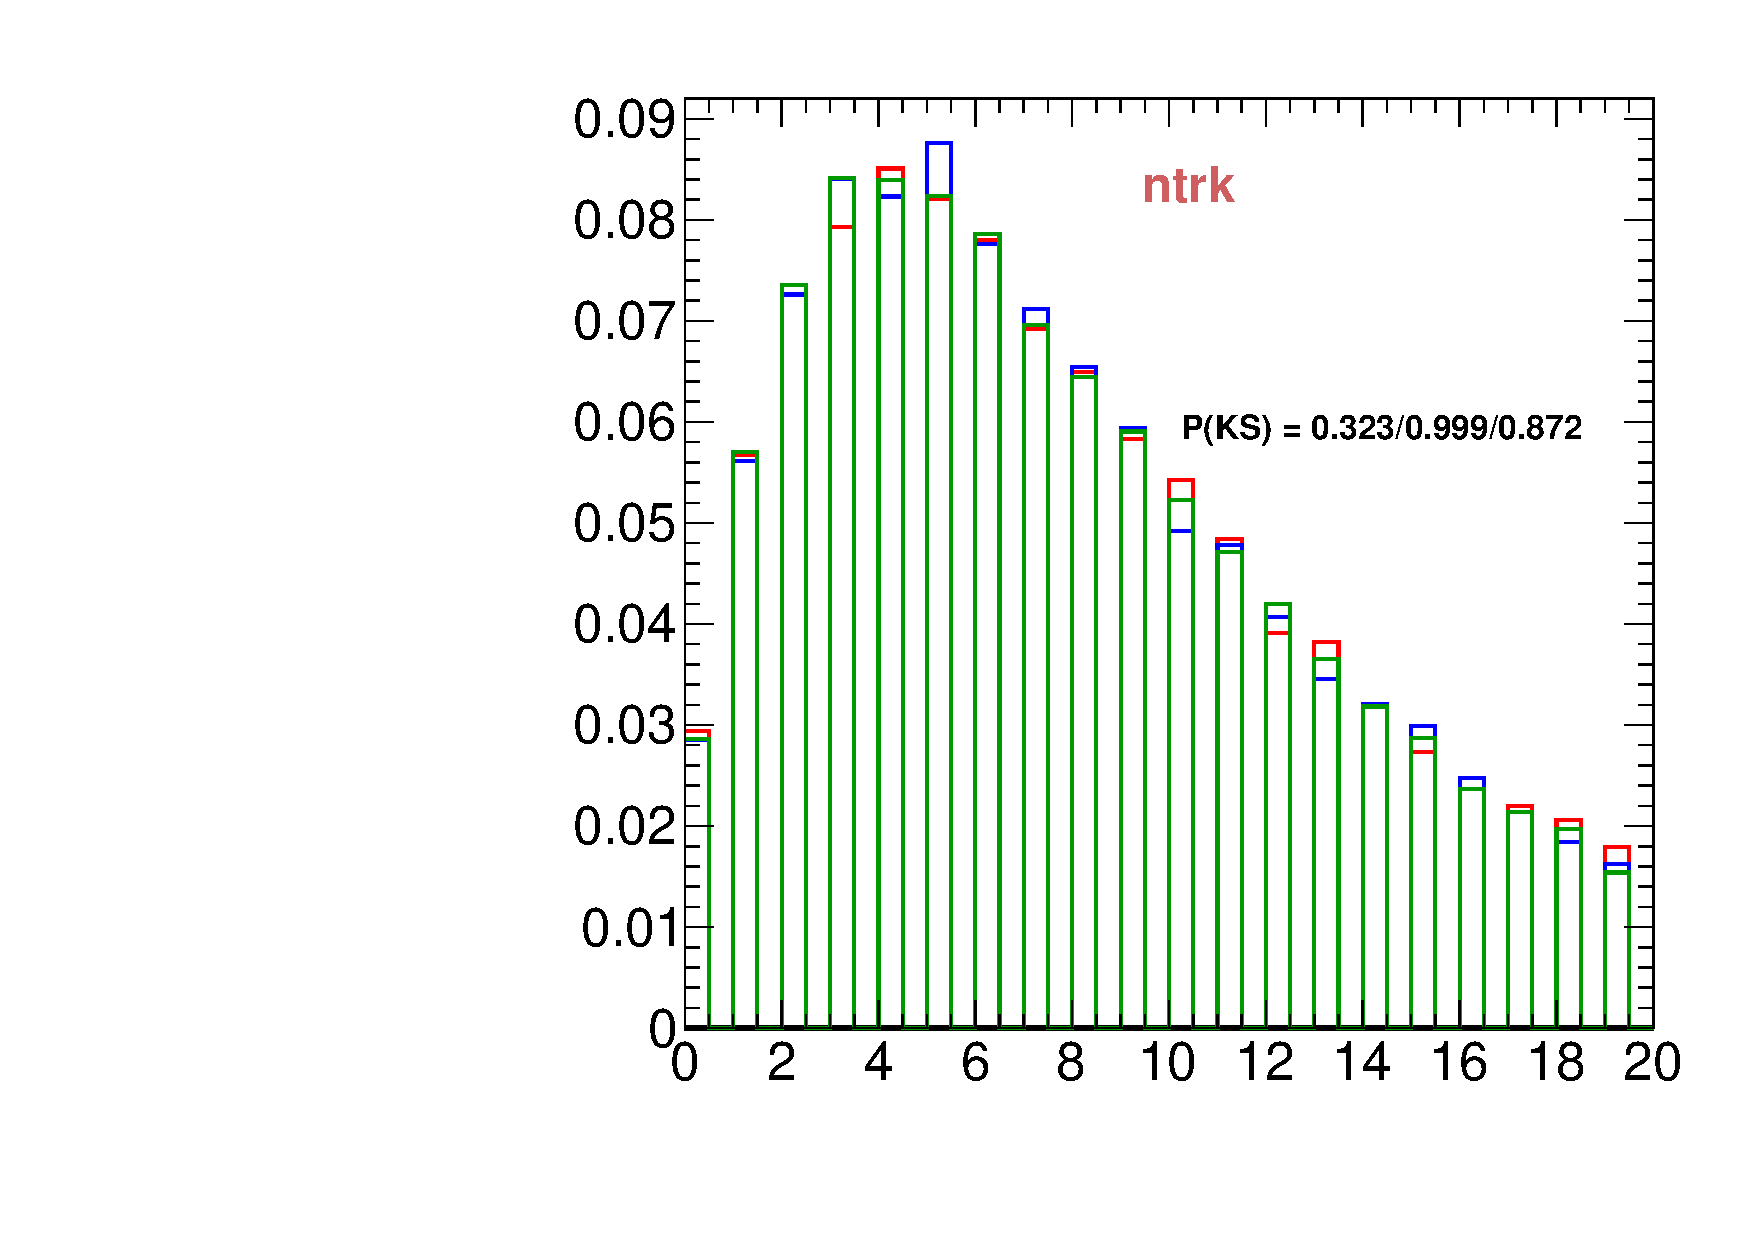
\includegraphics[width=\textwidth]{Figures/VariablesComparison/Data_endcaps_figs_3h/ntrk}
                \label{fig:Data_endcaps_ntrk_3h}
        \end{subfigure}
        \begin{subfigure}[b]{0.2\textwidth}
                \centering
                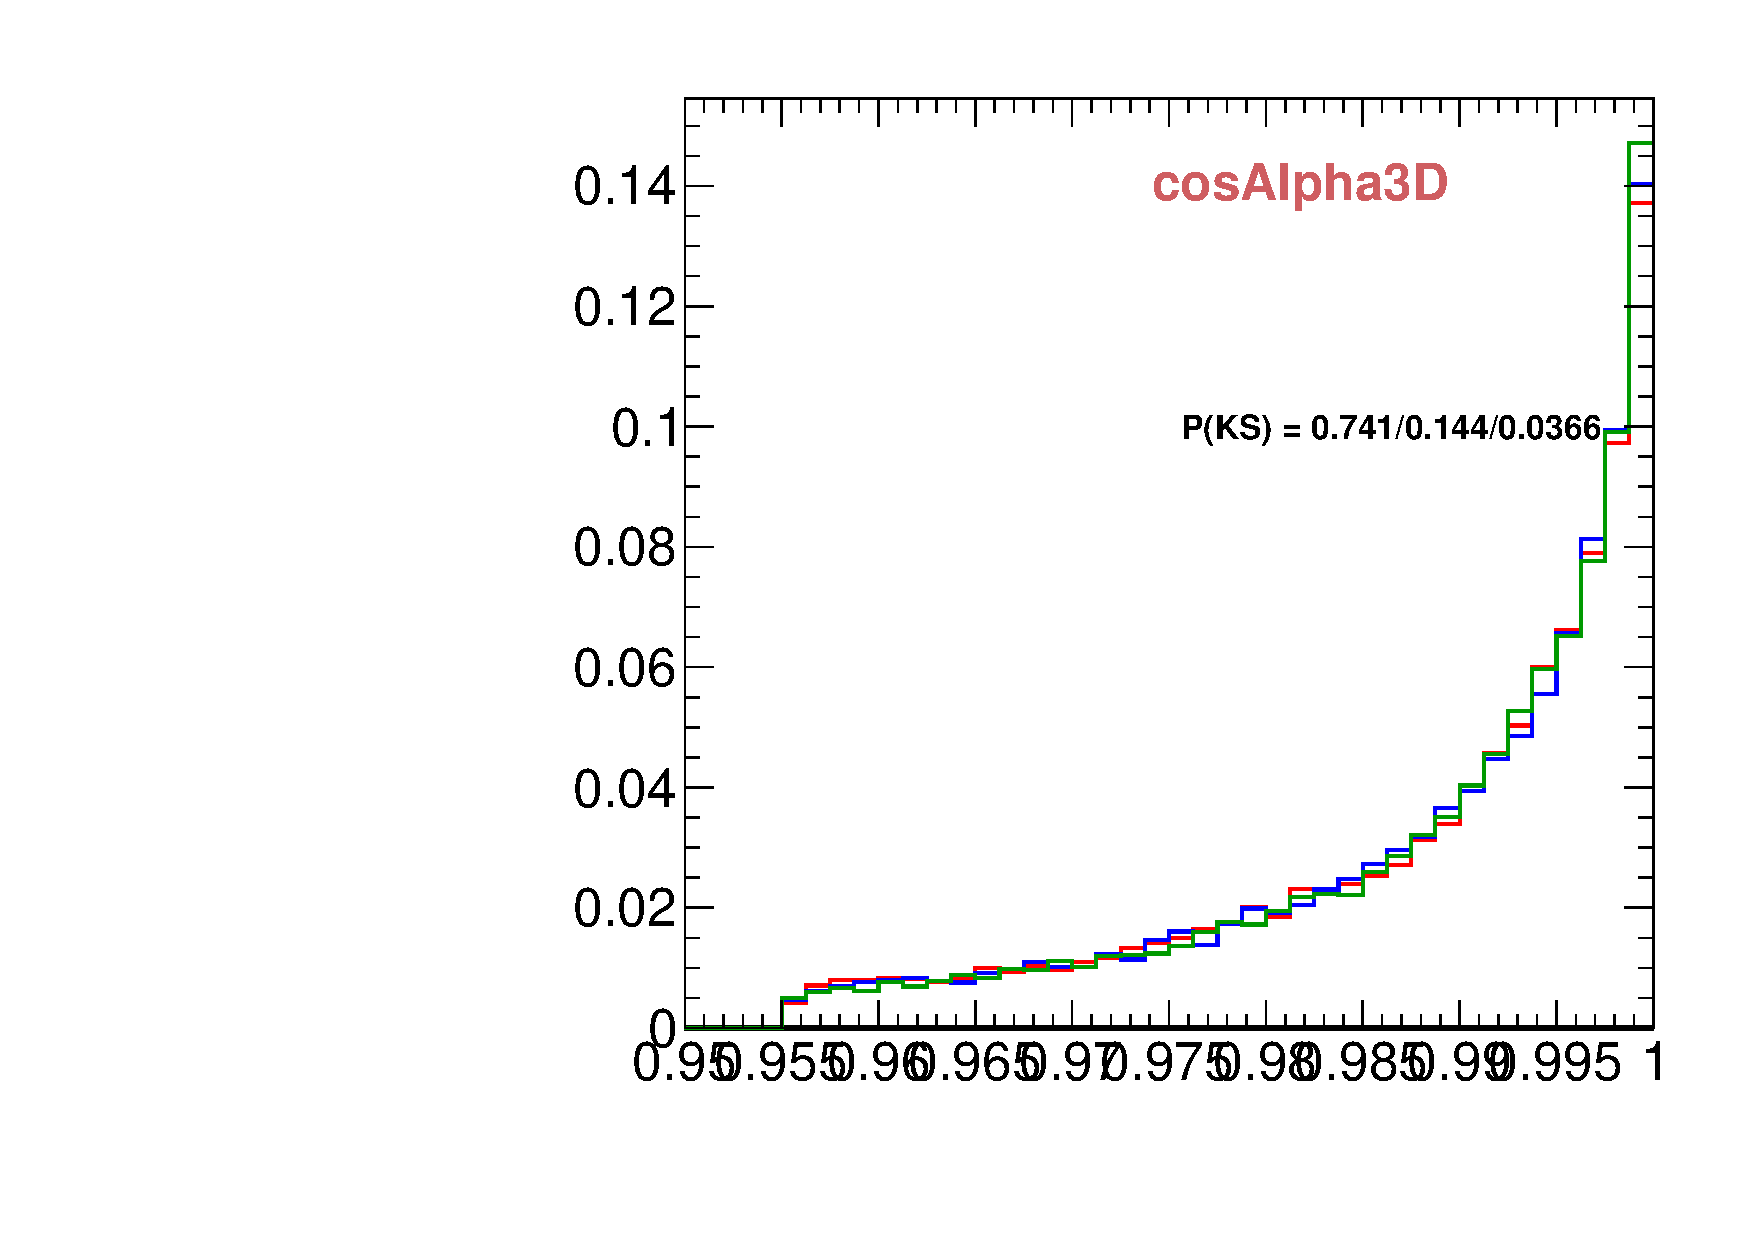
\includegraphics[width=\textwidth]{Figures/VariablesComparison/Data_endcaps_figs_3h/cosAlpha3D}
                \label{fig:Data_endcaps_cosAlpha3D_3h}
        \end{subfigure}
        \begin{subfigure}[b]{0.2\textwidth}
                \centering
                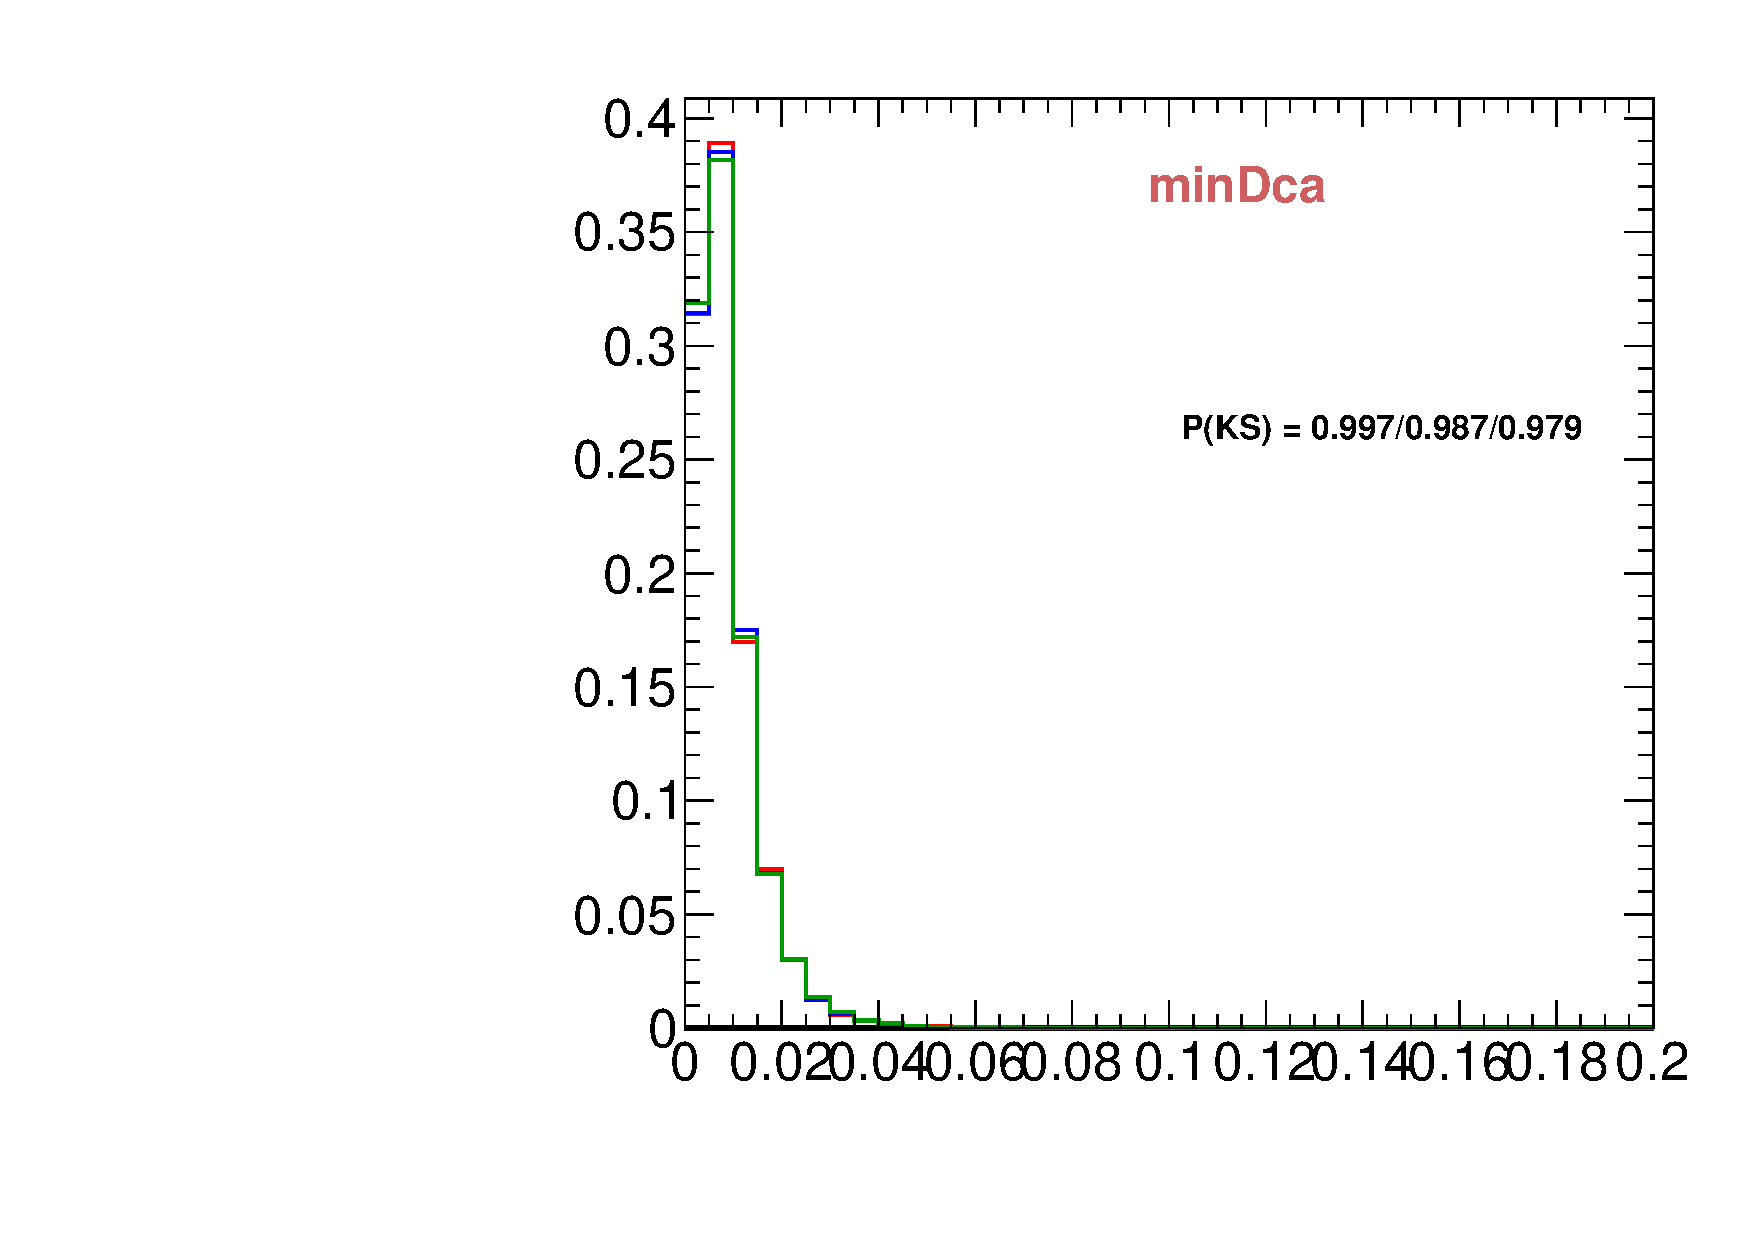
\includegraphics[width=\textwidth]{Figures/VariablesComparison/Data_endcaps_figs_3h/minDca}
                \label{fig:Data_endcaps_minDca_3h}
        \end{subfigure}
        \begin{subfigure}[b]{0.2\textwidth}
                \centering
                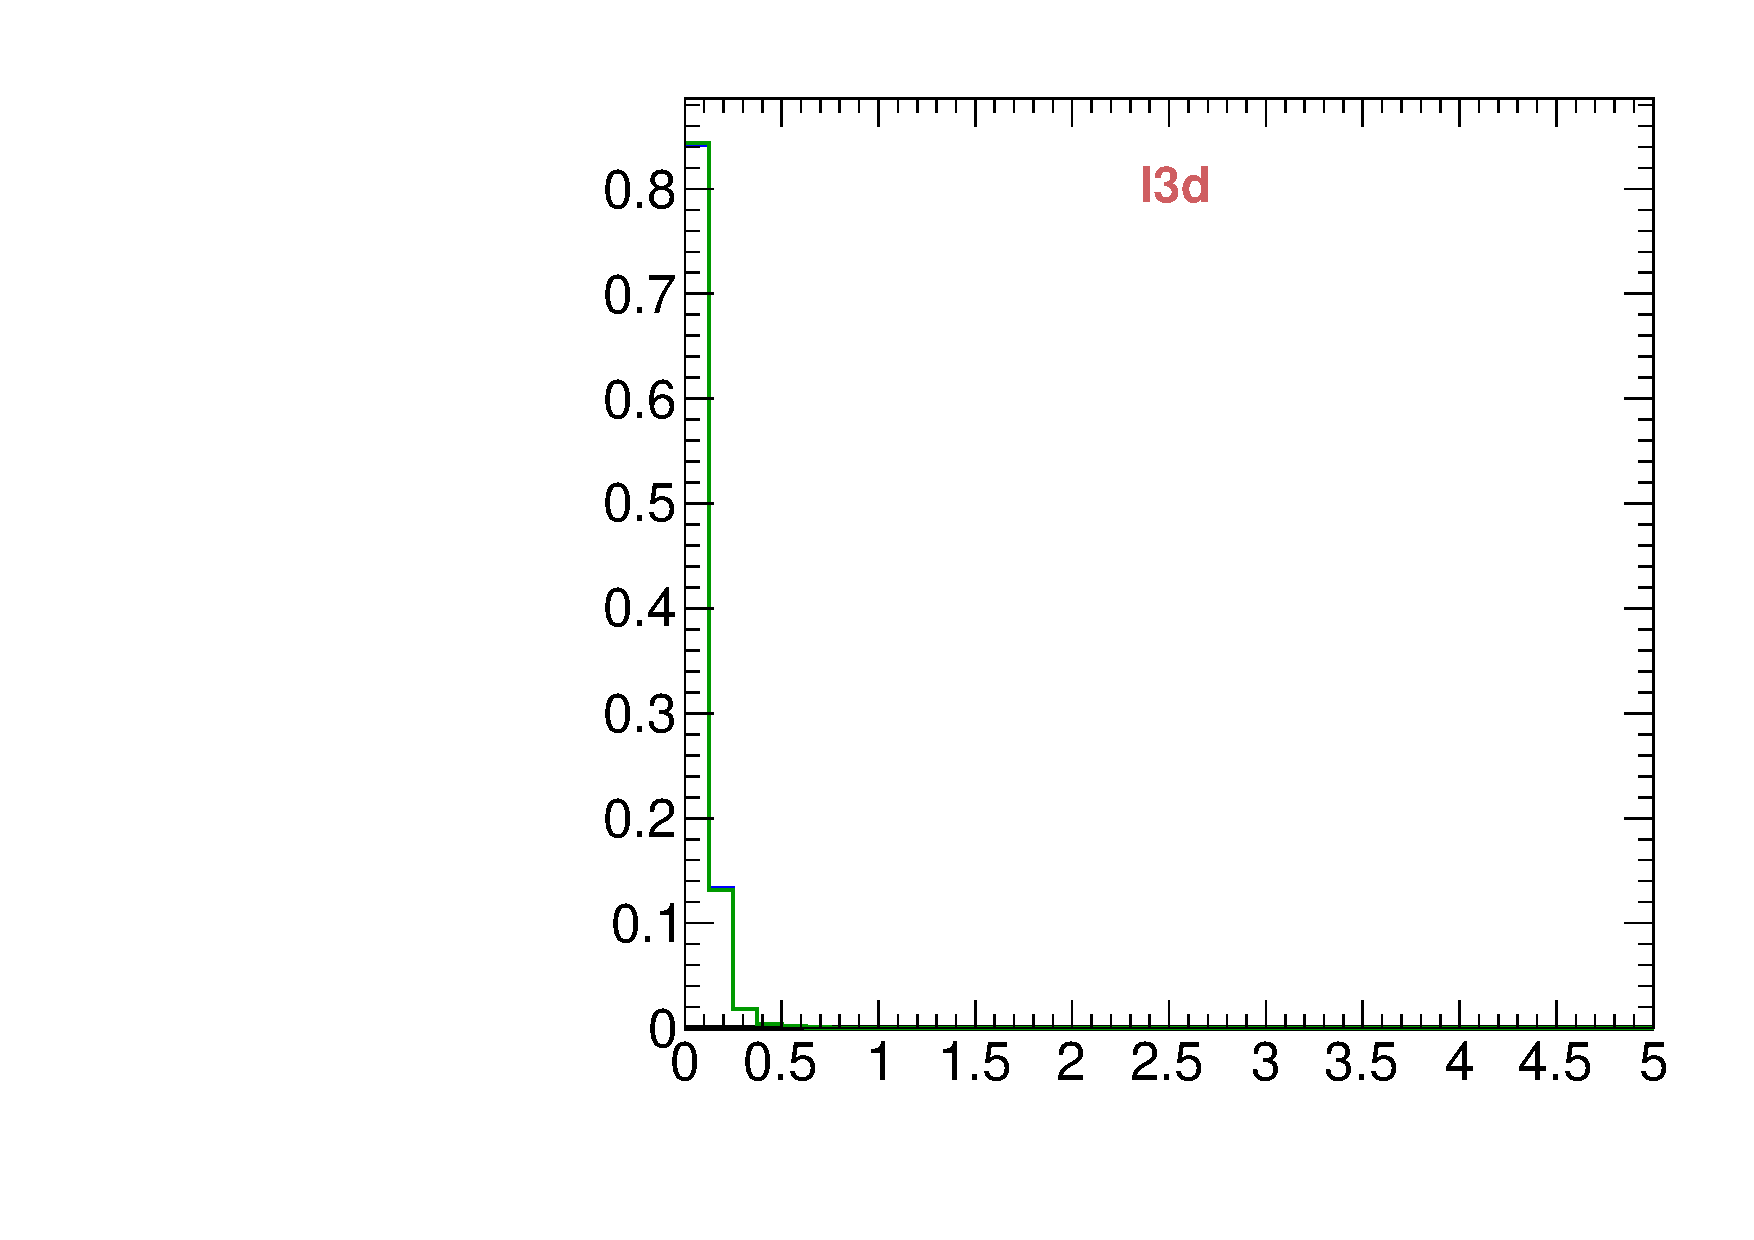
\includegraphics[width=\textwidth]{Figures/VariablesComparison/Data_endcaps_figs_3h/l3d}
                \label{fig:Data_endcaps_l3d_3h}
        \end{subfigure}
        \begin{subfigure}[b]{0.2\textwidth}
                \centering
                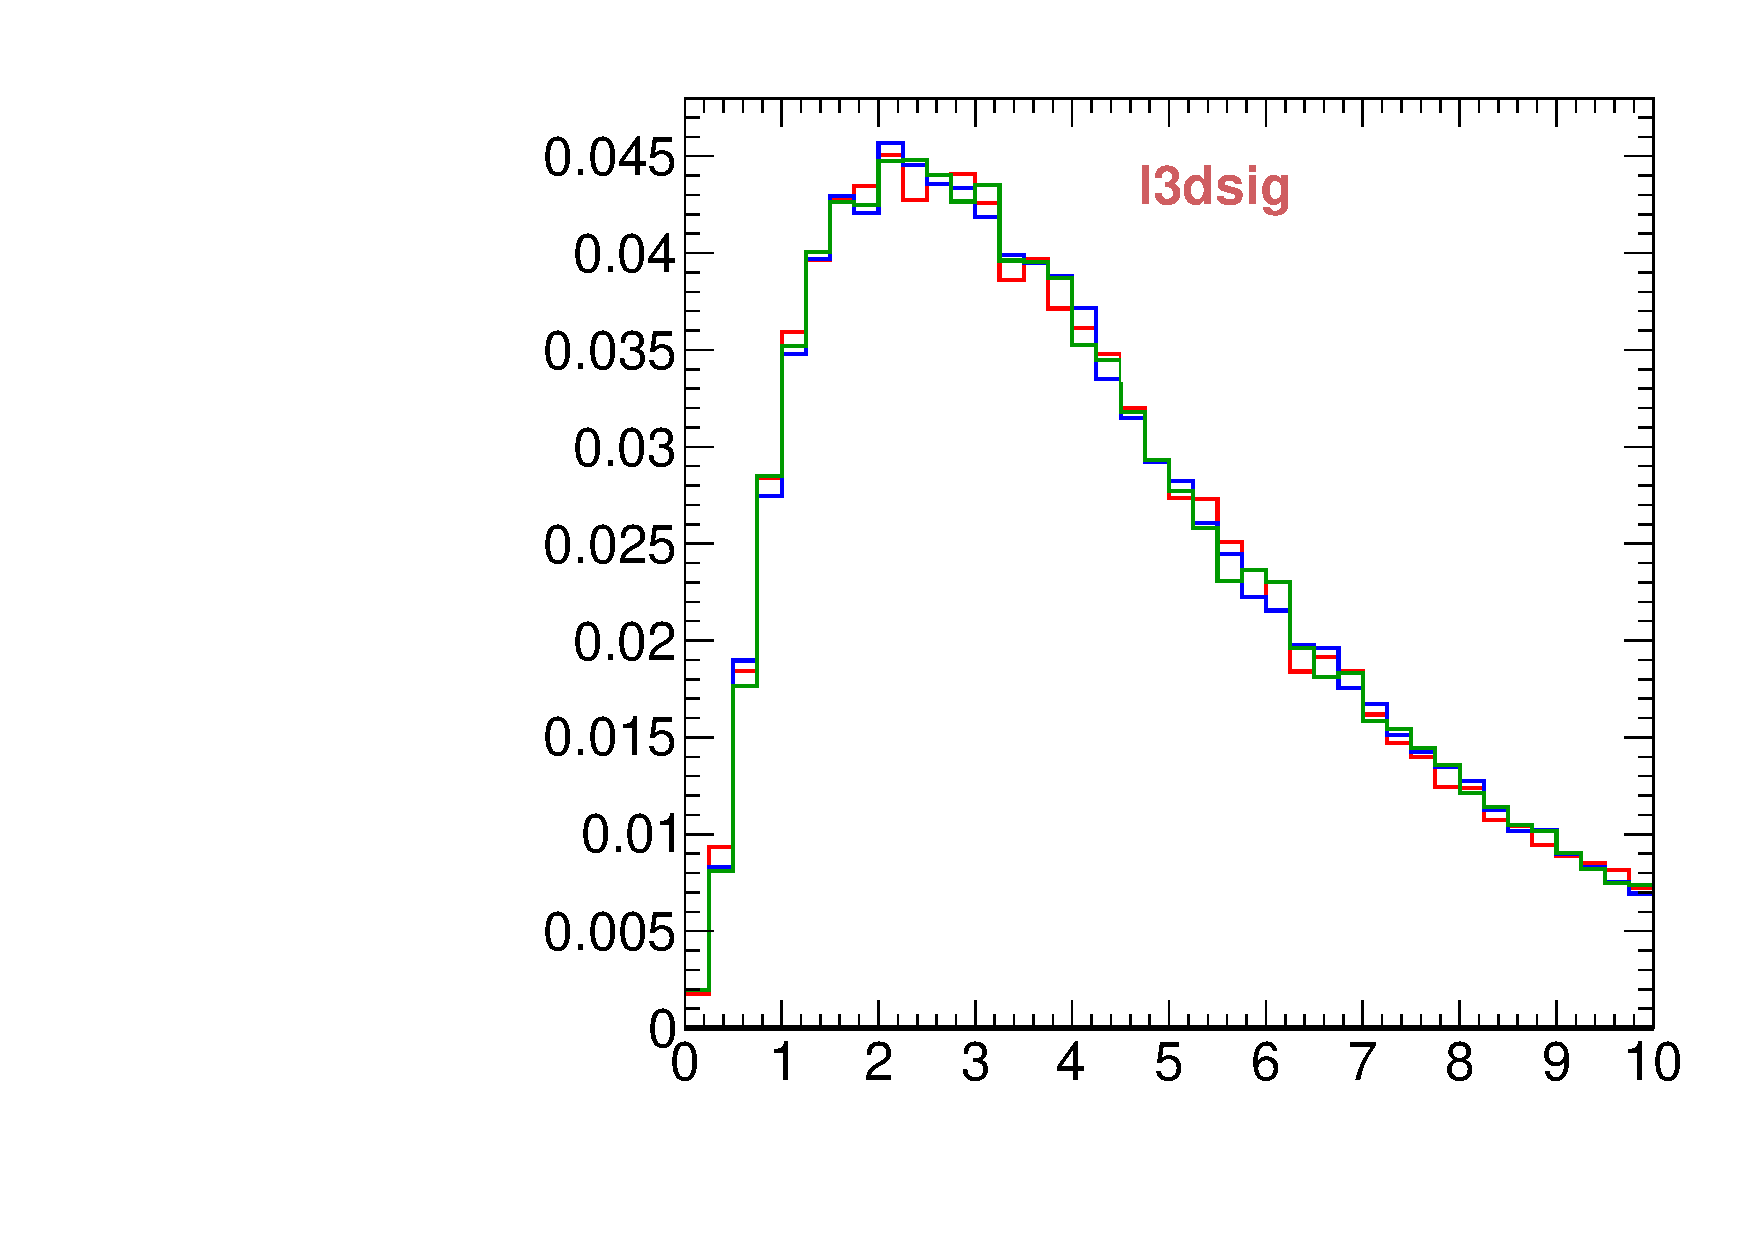
\includegraphics[width=\textwidth]{Figures/VariablesComparison/Data_endcaps_figs_3h/l3dsig}
                \label{fig:Data_endcaps_l3dsig_3h}
        \end{subfigure}
        \begin{subfigure}[b]{0.2\textwidth}
                \centering
                \includegraphics[width=\textwidth]{Figures/VariablesComparison/Data_endcaps_figs_3h/isolation}
                \label{fig:Data_endcaps_isolation_3h}
        \end{subfigure}
        \begin{subfigure}[b]{0.2\textwidth}
                \centering
                \includegraphics[width=\textwidth]{Figures/VariablesComparison/Data_endcaps_figs_3h/mass}
                \label{fig:Data_endcaps_mass_3h}
        \end{subfigure}
        \begin{subfigure}[b]{0.2\textwidth}
                \centering
                \includegraphics[width=\textwidth]{Figures/VariablesComparison/Data_endcaps_figs_3h/mu1_pt}
                \label{fig:Data_endcaps_mu1_pt_3h}
        \end{subfigure}
        \begin{subfigure}[b]{0.2\textwidth}
                \centering
                \includegraphics[width=\textwidth]{Figures/VariablesComparison/Data_endcaps_figs_3h/mu2_pt}
                \label{fig:Data_endcaps_mu2_pt_3h}
        \end{subfigure}
        \begin{subfigure}[b]{0.2\textwidth}
                \centering
                \includegraphics[width=\textwidth]{Figures/VariablesComparison/Data_endcaps_figs_3h/dca}
                \label{fig:Data_endcaps_dca_3h}
        \end{subfigure}
        \begin{subfigure}[b]{0.2\textwidth}
                \centering
                \includegraphics[width=\textwidth]{Figures/VariablesComparison/Data_endcaps_figs_3h/pt}
                \label{fig:Data_endcaps_pt_3h}
        \end{subfigure}
        \begin{subfigure}[b]{0.2\textwidth}
                \centering
                \includegraphics[width=\textwidth]{Figures/VariablesComparison/Data_endcaps_figs_3h/delta3d}
                \label{fig:Data_endcaps_delta3d_3h}
        \end{subfigure}
        \begin{subfigure}[b]{0.2\textwidth}
                \centering
                \includegraphics[width=\textwidth]{Figures/VariablesComparison/Data_endcaps_figs_3h/delta3dErr}
                \label{fig:Data_endcaps_delta3d/delta3dErr_3h}
        \end{subfigure}
        \begin{subfigure}[b]{0.2\textwidth}
                \centering
                \includegraphics[width=\textwidth]{Figures/VariablesComparison/Data_endcaps_figs_3h/pvw8}
                \label{fig:Data_endcaps_pvw8_3h}
        \end{subfigure}
        \begin{subfigure}[b]{0.2\textwidth}
                \centering
                \includegraphics[width=\textwidth]{Figures/VariablesComparison/Data_endcaps_figs_3h/KS}
                \label{fig:Data_endcaps_KS_3h}
        \end{subfigure}
        \caption{Overlay of BDT training variable distributions in data sideband background for events of the three subsets in the endcap. The plot on the bottom right summarizes all KS probablities.}
        \label{fig:Data_endcaps_figs_3h}
\end{sidewaysfigure}


